\documentclass[twoside,11pt]{article}
\usepackage{jair, theapa, rawfonts}
\usepackage{amsmath,amsfonts,amssymb,amsthm}
\usepackage[vlined,algoruled,titlenumbered,noend]{algorithm2e}
\usepackage{array}
\usepackage{epsfig,subfigure,graphicx}

\def\argmax{\operatornamewithlimits{arg\max}}
\newcommand{\casemax}{\mathrm{casemax}}
\newcommand{\MarsRover}{\textsc{Mars Rover }}
\newcommand{\casemin}{\mathrm{casemin}}
\newcommand{\UB}{\mathit{UB}}
\newcommand{\LB}{\mathit{LB}}
\newcommand{\IND}{\mathit{Ind}}
\newcommand{\CONS}{\mathit{Cons}}
\newcommand{\Root}{\mathit{Root}}
\newcommand{\Max}{\mathit{Max}}
\newcommand{\sq}{\hspace{-1mm}}
\newcommand{\sqm}{\hspace{-2mm}}
\newcommand{\true}{\mathit{true}}
\newcommand{\false}{\mathit{false}}
\newcommand{\Knapsack}{\textsc{Knapsack}}
\newcommand{\MarsRoverL}{\textsc{Mars Rover Linear }}
\newcommand{\MarsRoverNL}{\textsc{Mars Rover Nonlinear }}
\newcommand{\InventoryControl}{\textsc{Inventory Control }}
\newcommand{\WaterReservoir}{\textsc{Reservoir Management }}
\newcommand{\MultiWaterReservoir}{\textsc{Multi-Reservoir }}
\newtheorem*{example*}{Example}
\newtheorem{theorem}{Theorem}[section]
\newtheorem{corollary}{Corollary}[section]
\newtheorem{lemma}{Lemma}[section]
\newtheorem{example}[lemma]{Example}

\newenvironment{mydef}[1][Definition]{\begin{trivlist}
\item[\hskip \labelsep {\bfseries #1}]}{\end{trivlist}}

%\jairheading{1}{1993}{1-15}{6/91}{9/91}
\ShortHeadings{Exact Symbolic Solutions to MDPs}
{Zamani, Sanner}
%\firstpageno{25}


\begin{document}

\title{Exact Symbolic Dynamic Programming for Hybrid State and Action MDPs}

\author{\name Zahra Zamani \email zahra.zamani@anu.edu.au \\
       \name Scott Sanner \email ssanner@nicta.com.au \\
       \addr The Australian National University and NICTA,\\
       Canberra, ACT 0200 Australia       
}

\maketitle


\begin{abstract}
Many real-world decision-theoretic planning problems can naturally be modeled using continuous states and actions. Problems such as the multi-item Inventory problem \cite{Scarf_Karlin58} have long been solved in the operation research literature using discrete variable MDPs or approximating the optimal value for continuous domains. Other work similar to that of Gaussian control deals with general continuous domains but can not handle piecewise values on the state space. Here we propose a framework to find the first exact optimal piecewise solution for problems modeled using multi-variate continuous state and action variables.

We define a Symbolic Dynamic Programming (SDP) approach using the \emph{case} calculus which provides a closed-form solution for all operations (e.g. continuous maximization and integration). Solutions are provided for discrete action Hybrid(i.e. discrete and continuous) state MDPs (HMDPs) using polynomial transitions with discrete noise and arbitrary reward functions . Solutions to continuous action HMDPs with piecewise linear (or quadratic) discrete noise transition and reward functions are also derived. 

Apart from providing the solution to general HMDPs, our other contribution is the compact representation of XADDs - a continuous variable extension of Algebraic decision diagrams (ADDs) - with related properties and algorithms. This allows us to empirically provide efficient results for HMDPs showing the \emph{first optimal automated solution} on various continuous domains. 
\end{abstract}

\section{Introduction}
\label{Introduction}
Many stochastic planning problems in the real-world involving resources, time, or spatial configurations naturally use continuous variables in their state representation.  For example, in the \MarsRover\  problem \cite{bresina02}, a rover must manage bounded continuous resources of battery power and daylight time as it plans scientific discovery tasks for a set of landmarks on a given day. A rover can also have continuous actions in navigating (moving continuously). 

Other examples include \InventoryControl\ problems \cite{Scarf_Karlin58} for continuous resources such as petroleum products, a business must decide what quantity of each item to order subject to uncertain demand, (joint) capacity constraints, and reordering costs; and  \WaterReservoir\ problems \cite{reservoir}, where a utility must manage continuous reservoir water levels in continuous time to avoid underflow while maximizing electricity generation revenue.

%While all these problems are naturally modeled using discrete action hybrid (discrete and continuous) state Markov Decision Processes (DA-HMDPs) or continuous action hybrid MDPs (CA-HMDPs), there has been no prior work handling piecewise transitions. 
%more here?
Little progress has been made in the recent years in developing \emph{exact} solutions for HMDPs with multiple continuous state variables beyond the subset of HMDPs  which have an optimal \emph{hyper-rectangular piecewise linear value function} \cite{feng04,li05}. Further previous work on \emph{exact} solutions to multivariate continuous state \emph{and} action settings have been limited to the control theory literature for the case of linear-quadratic Gaussian (LQG) control \cite{lqgc}. 
%i.e., minimizing a quadratic cost function subject to linear dynamics with Gaussian noise in a partially observed setting.  
However, the transition dynamics and reward (or cost) for such problems cannot be piecewise --- a crucial limitation preventing the application of such solutions to many planning and operation research (OR) problems. 
Consider the famous OR problem of \InventoryControl in \cite{Scarf_Karlin58}: 
\begin{example*} [\InventoryControl]
Inventory control problems -- how much of an
item to reorder subject to capacity constraints, demand, and optimization criteria-- date back to the 1950's with Scarf's optimal solution to the \emph{single-item capacitated inventory control} (SCIC) problem.
\emph{Multi-item joint capacitated inventory (MJCIC) control} -- with upper limits
on the total storage of all items-- has proved to be an NP-hard problem and
as a consequence, most solutions resort to some form of
approximation \cite{bitran,wusd10}; indeed, we are unaware of any 
work which claims to find an exact closed-form non-myopic
optimal policy for \emph{all} (continuous) inventory states for MJCIC 
under linear reordering costs and linear holding costs.
\end{example*}

Consider a continuous state version of this problem with discrete actions: 
\vspace{2mm}

\textsc{Discrete Action} \InventoryControl (\textsc{DAIC}): 
A multi-item ($K$-item) inventory consists of continuous amounts of specific items $x_i$ where $i \in [0,K]$ is the number of items and $x_i \in [0,200]$. The customer demand is a stochastic boolean variable $d$ for low or high demand levels.  Ordering a specific item $a_j$ comes in three discrete ranges of  $(low,mid, high)$ where $\lbrace low = 25, mid = 50, high = 75 \rbrace$ and $j \in \lbrace 1,2,3 \rbrace$. There are linear reorder costs and also a penalty for holding items. The transition and reward functions have to be defined for each continuous item $x_i$ and action $j$.
%is this good? do I need to put transition and reward? 

We can also consider the more general  continuous action HMDP setting to this problem: 
\vspace{2mm}

\textsc{Continuous Action}  \InventoryControl (\textsc{CAIC}):
Here in a given time step, the inventory can order  any of the $i$ items $a_i \in [0,200]$ considering the stochastic customer demand. 

The transition functions for the continuous state $x_i$ and actions $a_i$ is defined as: 
{%\footnotesize
\vspace{-2mm}
\begin{align}
x'_i= \begin{cases}
d  : & x_i + a_i - 150 \\
\neg d : & x_i + a_i - 50    
\end{cases} %\label{eq:trans_inv}
\hspace{4mm}
 P(d'=\mathit{true}|d,\vec{x},\vec{x'})=  \begin{cases}
d     :& 0.7\\
\neg d : & 0.3	\\
\end{cases} \label{eq:transD_inv}
\end{align}
\vspace{-2mm}}

The reward is the sum of $K$ functions $R = \sum_{i=0}^K R_i $ as below:
{\footnotesize
\begin{align}
R =
\begin{cases}
\sum_{j} x_j \geq C &: -\infty  \\	
\sum_{j} x'_j \geq C &: -\infty 	\\
\sum_{j} x_j \leq C &:0\\  
\sum_{j} x'_j \leq C &: 0 	\\
\end{cases}
+
\Bigg( \sum_{i=0}^K \begin{cases}
d \wedge x_i \geq 150&: 150 - 0.1 * a_i - 0.05 * x_i \\
d \wedge x_i \leq 150 &:   x_i - 0.1 * a_i - 0.05 * x_i \\
\neg d \wedge x_i \geq 50 &: 50 - 0.1 * a_i - 0.05 * x_i  \\
\neg d \wedge x_i \leq 50 &: x_i - 0.1 * a_i - 0.05 * x_i  \\
\end{cases} 
+ 
\begin{cases}
x_i \leq 0 &: -\infty  \\	
x'_i \leq 0&: -\infty  \\	
x_i \geq 0 &:0\\
x'_i \geq 0 &: 0
\end{cases} \Bigg)
\label{rew_inv}
\end{align}}
where $C$ is the total capacity for $K$ items in the inventory. The first and last cases check the safe ranges of the capacity such that the inventory capacity of each item above zero and the sum of total capacity below $C$ is desired.
%%%%%%%%%%%%%%%%%%%%%%%%%%%%%%%%%%%%%%%%%%%%%%%%%%%%%%%%%%%%%%%%%%%%%%%%%%
%\vspace{5mm}
\begin{figure}[t!]
\centering
%\subfigure{
%\hspace{-20mm}
%\vspace{-3mm}
%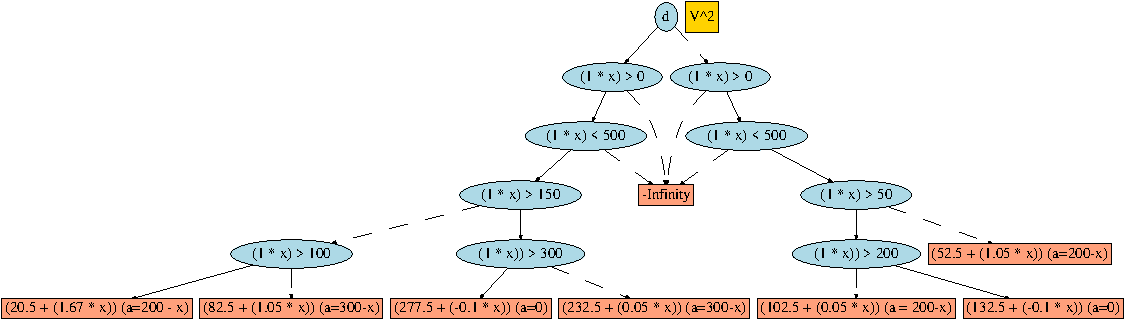
\includegraphics[width=1 \textwidth]{Figures2/diagrams/v2_inv2_2.pdf}
\begin{subfigure}
                \centering
                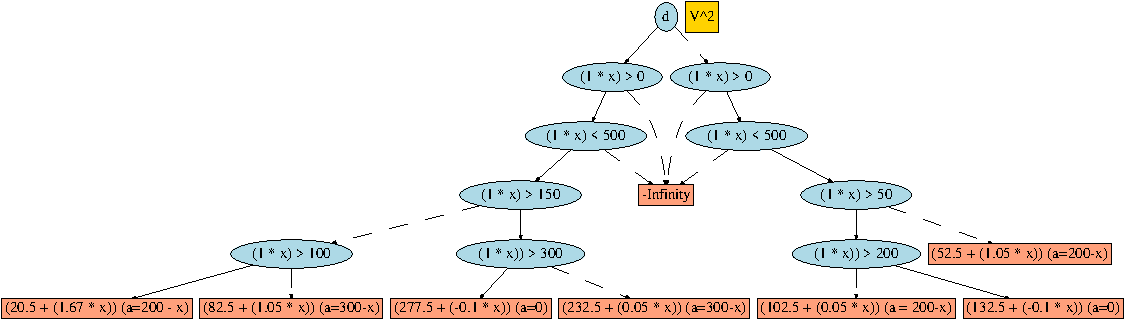
\includegraphics[width=0.77\textwidth]{Figures2/diagrams/v2_inv2_2.pdf}
        \end{subfigure}
                \hspace{2mm}
\begin{subfigure}
                \centering
                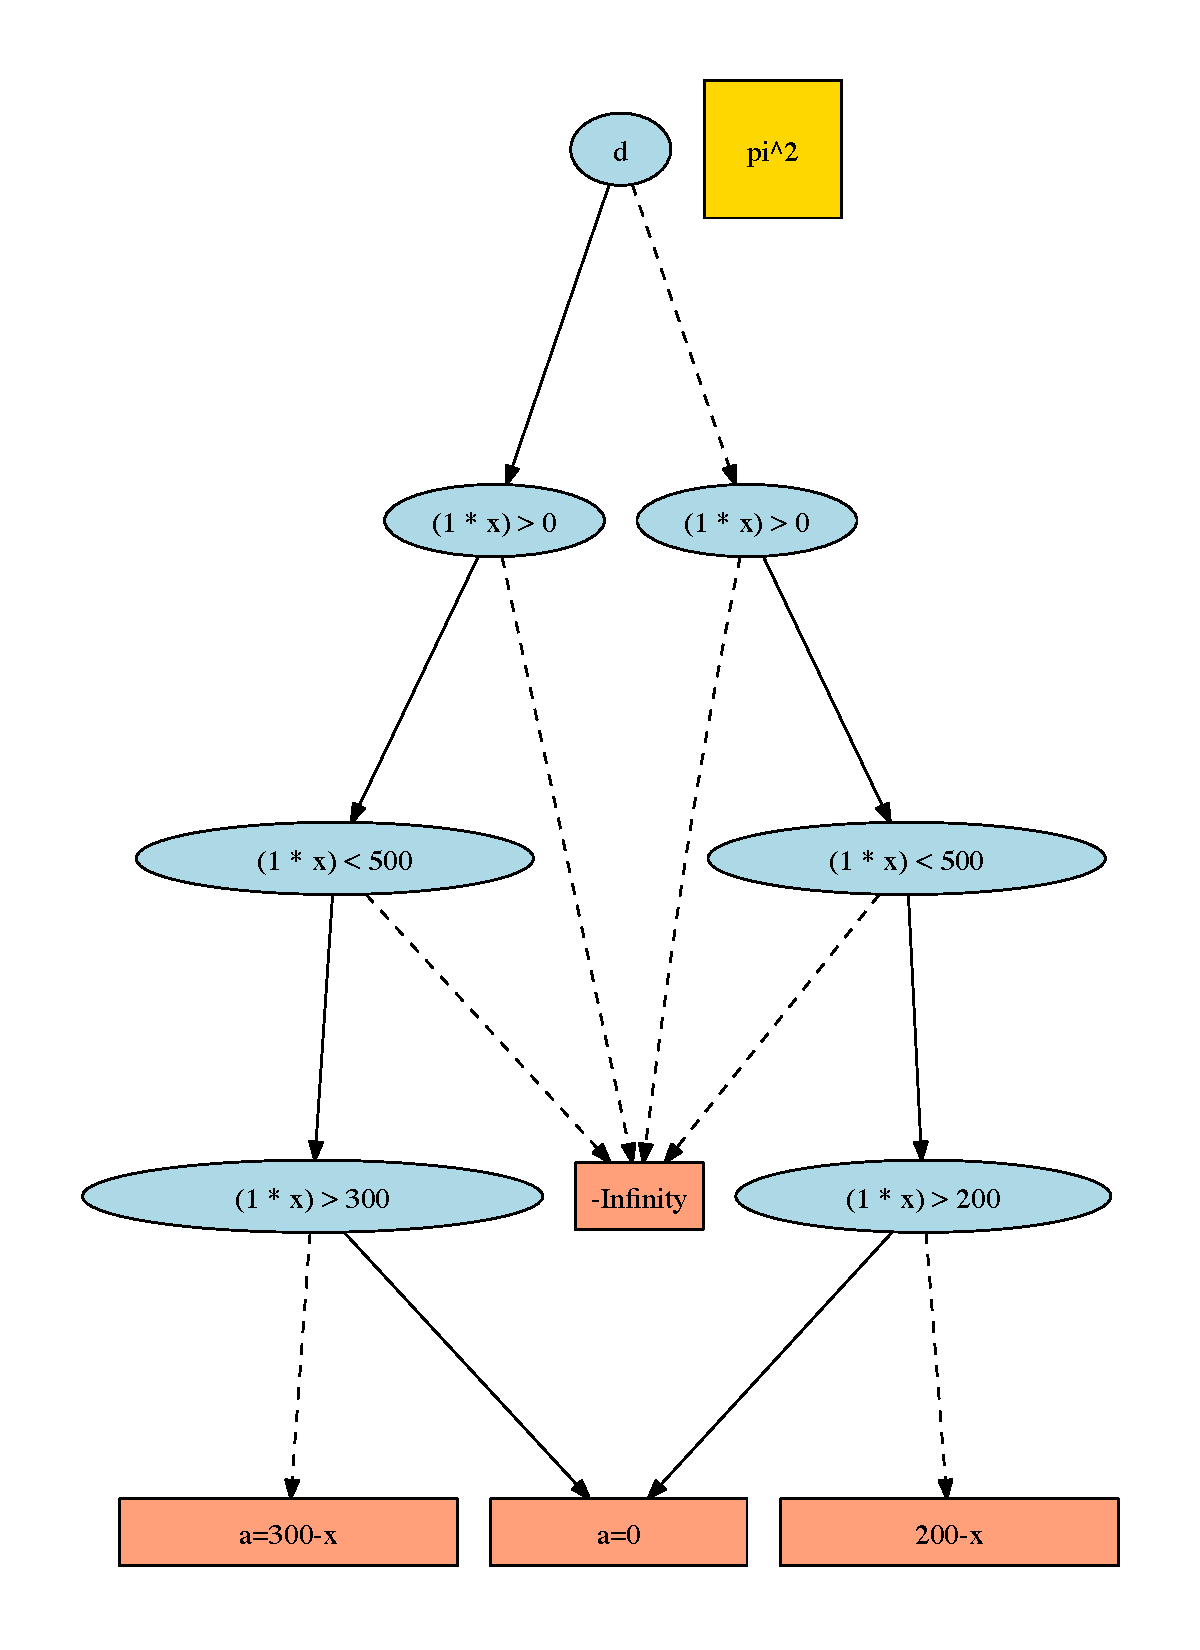
\includegraphics[width=0.18\textwidth]{Figures2/diagrams/p2_inv_2.pdf}
        \end{subfigure}
%\vspace{-2mm}
\caption{\footnotesize Optimal value function $V^2(x)$ for the
CAIC problem represented as an extended algebraic decision
diagram (XADD).  Here the solid lines represent the $\true$ branch for
the decision and the dashed lines the $\false$ branch.  To evaluate
$V^2(x)$ for any state $x$, one simply traverses the diagram in a
decision-tree like fashion until a leaf is reached where the
non-parenthetical expression provides the \emph{optimal value} and the
parenthetical expression provides the \emph{optimal policy} 
($a = \pi^{*,2}(x)$) to achieve value $V^2(x)$ (Left); Optimal policy for the second iteration $\pi^2$ consistent with Scarf's policy (Right).}
\label{fig:inv_policy}
\vspace{-7mm}
\end{figure}
%%%%%%%%%%%%%%%%%%%%%%%%%%%%%%%%%%%%%%%%%%%%%%%%%%%%%%%%%%%%%%%%%%%%%%%%%%
Note that illegal state values are defined using $-\infty$, in this case having the capacity lower than zero at any time and having capacity higher than that of the total $C$. If our objective is to maximize the long-term \emph{value} $V$ (i.e.,the sum of rewards received over an infinite horizon of actions), we show that the optimal value function can be derived in closed-form. 
For a single-item continuous state and action inventory CAIC problem the optimal value function is defined as below:
\vspace{-1mm}
\begin{align}
V = \begin{cases}
(x < 0 \vee x>500) &: -\infty \\
d \land (0 \leq x \leq 500) \land (x \geq 300) &:  277.5 - 0.1 * x \\
d \land (150 \leq x \leq 300) &:  232.5 + 0.05 * x \\
d \land (100 \leq x \leq 150) &:  20.5 + 1.67 * x\\
d \land (0 \leq x \leq 100) &:  82.5 + 1.05 * x \\
\neg d \land (200 \leq x \leq 500)  &:  132.5 - 0.1 * x \\
\neg d \land (50 \leq x \leq 200) &: 102.5 + 0.05 * x \\
\neg d \land (0 \leq x \leq 50) &:  52.5 + 1.05 * x \\
\end{cases} \label{eq:vfun_inv}
\vspace{-8mm}
\end{align}
This value function is piecewise and linear and the policy obtained from this value function shown in Figure ~\ref{fig:inv_policy} (for each slice of the state space) matches with Scarf's policy for the \InventoryControl problem. If the holding and storage costs are linear, the optimal policy in each horizon is always of $(S,s)$ ~\cite{Scarf_Karlin58}. In general this means if ($x>s$) the policy should be not to order any items and if ($x<s$) then ordering $S-s-x$ items is optimal. Figure~\ref{fig:inv_policy} represents an extended algebraic decision diagram (XADD) representation which allows efficient implementation of the \emph{case calculus} for arbitrary functions. 
%%%%%%%%%%%%%%%%%%%%%%%%%%%%%%%%%%%%
According to this we rewrite Scarf's policy: 
\begin{align}
\pi^{*,2}(x) = 
\begin{cases}
(x < 0 \vee x>500) &: -\infty \\
d \land (300 \leq x \leq 500)  &:  0 \\
d \land (0 \leq x \leq 300) &:  300 - x \\
d \land (100 \leq x \leq 150)  &:  200 - x \\
\neg d \land (200 \leq x \leq 500) &:  0 \\
\neg d \land (0 \leq x \leq 200) &:  200 - x \\
\end{cases}
\end{align}

While this simple example illustrates the power of using continuous variables, for a multi-variate problem it is the very first solution to exactly solving problems such as the CAIC. 

We propose novel ideas to work around some of the expressiveness limitations of previous approaches and significantly generalize the range of HMDPs that can be solved exactly.  To achieve this more general solution, this
paper contributes a number of important advances:
\begin{itemize}
\item The use of case calculus allows us to perform Symbolic dynamic programming (SDP) \cite{fomdp} used to solve MDPs with
piecewise transitions and reward functions defined in first-order logic. We define all required operations for SDP such as $\oplus,\ominus,max,min$ as well as new operations such as the continuous maximization of an action parameter $y$ defined as $max_y$ and integration of discrete noisy transition.
\item We perform value iteration for two different settings. In the first setting of DA-HMDP we consider continuous state variables with a discrete action set while in the second setting CA-HMDP we consider continuous states and actions. Both DA-HMDPs and CA-HMDPs are evaluated on various problem domains. The results show that DA-HMDPs applies to a wide range of transition and reward functions providing hyper-rectangular value functions. CA-HMDPs have more restriction in modeling due to the increased complexity caused by continuous actions, and limit solutions to linear and quadratic transitions and rewards but provide strong results for many problems never solved exactly before. 
\item While the \emph{case} representation for the optimal \textsc{CAIC} 
solution shown in \eqref{eq:vfun_inv} is sufficient in theory to
represent the optimal value functions that our HMDP solution
produces, this representation is unreasonable to maintain in practice
since the number of case partitions may grow exponentially on
each receding horizon control step.  For \emph{discrete} factored
MDPs, algebraic decision diagrams (ADDs) \cite{bahar93add} have been
successfully used in exact algorithms like SPUDD \cite{spudd} to
maintain compact value representations.  Motivated by this work we
introduce extended ADDs (XADDs) to compactly represent general
piecewise functions and show how to perform efficient operations on
them \emph{including} symbolic maximization.  Also we present all properties and algorithms required for XADDs. 
\end{itemize}

Aided by these algorithmic and data structure advances, we empirically demonstrate that our SDP approach with XADDs can exactly solve a variety of HMDPs with discrete and continuous actions. 


\section{Hybrid MDPs (HMDPs)}
The mathematical framework of Markov Decision Processes (MDPs) is used for modelling many stochastic sequential decision making problems ~\cite{bellman}. This discrete-time stochastic control process chooses an action $a$ available at state $s$. The process then transitions to the next state $s'$ according to $T(s,s')$ and receives a reward $R(s,a)$. The transition function follows the Markov property allowing each state to only depend on its previous state.  We provide novel exact solutions using the MDP framework for discrete and continuous variables in the state and action space. Hybrid State and Action MDPs (HMDPs) are introduced in the next section followed by the finite-horizon solution via dynamic programming ~\cite{li05}.
%\vspace*{-0.05in}
\subsection{Factored Representation}
\label{sec:HMDPs}
%\vspace*{-0.05in}
In an HMDP, states are represented by vectors of variables
$(\vec{b},\vec{x}) = ( b_1,\ldots,b_n,x_{1},\ldots,x_m )$.  We assume
that each $b_i \in \{ 0,1 \}$ ($1 \leq i \leq n$) is boolean$\,$
and each $x_j \in \mathbb{R}$ ($1 \leq j \leq
m$) is continuous.  We also assume a finite set of $p$ actions 
%$A = \{a_{c1}(\vec{y}_1), \ldots, a_{cp}(\vec{y}_p), a_{d1},\ldots, a_{dp}\}$
$A = \{a_{1}(\vec{y}_1), \ldots, a_{p}(\vec{y}_p)\}$, where each action $a_k(\vec{y_k})$ ($1
\leq k \leq p$)  with parameter $\vec{y}_k \in \mathbb{R}^{|\vec{y}_k|}$  denotes continuous parameters for 
action $a_{k}$ and  if $|\vec{y}_k|=0$ then action $a_{k}$ has no parameters and is a discrete action.

Each HMDP model requires the following definitions: 

(i) a state transition model $P(\vec{b}',\vec{x}'|\vec{b},\vec{x},a,\vec{y})$, which specifies the
probability of the next state $(\vec{b}',\vec{x}')$ conditioned on a
subset of the previous and next state and action $a$ with its possible parameters $\vec{y}$; 

(ii) a reward function $R(\vec{b},\vec{x},\vec{b}',\vec{x}',a,\vec{y})$, which specifies the immediate reward obtained by taking action $a(\vec{y})$ in state $(\vec{b},\vec{x})$; 

(iii) a discount factor $\gamma, \; 0 \leq \gamma \leq 1$ to determine the weights of rewards in each time step.
\footnote{If time is explicitly included as one of the
continuous state variables, $\gamma = 1$ is typically used, unless
discounting by horizon (different from the state variable time) is
still intended.}  

A policy $\pi$ specifies the action $a(\vec{y}) =\pi(\vec{b},\vec{x})$ to take in each state $(\vec{b},\vec{x})$.  Our
goal is to find an optimal sequence of finite horizon-dependent
policies
%put footnote back in
\footnote{We assume a finite horizon $H$ in this
paper, however in cases where our SDP algorithm converges
in finite time, the resulting value function and 
corresponding policy are optimal for $H=\infty$. 
For finitely bounded value
with $\gamma = 1$, the forthcoming SDP algorithm may terminate in
finite time, but is not guaranteed to do so; for $\gamma < 1$, an
$\epsilon$-optimal policy for arbitrary $\epsilon$ can be computed by
SDP in finite time.
} 
$\Pi^* = (\pi^{*,1},\ldots,\pi^{*,H})$ that
maximizes the expected sum of discounted rewards over a horizon $h \in H; H \geq 0$:
\begin{align}
V^{\Pi^*}(\vec{x}) & = E_{\Pi^*} \left[ \sum_{h=0}^{H} \gamma^h \cdot r^h \Big| \vec{b}_0,\vec{x}_0 \right]. \label{eq:vfun_def}
\end{align}
Here $r^h$ is the reward obtained at horizon $h$ following $\Pi^*$ where 
we assume starting state $(\vec{b}_0,\vec{x}_0)$ at $h=0$.

 %%%%%%%%%%%%%%%%%%%%%%%%%%%%%%%%%%%%%%%%%%%%%%%%%%%%%%%%%%%%%%%%%%%%%%%%%%
%\vspace{10mm}
\begin{figure}[t!]
%\centering
%\subfigure{
%\hspace{-20mm}
%\vspace{-6mm}
 \begin{subfigure}
                \centering
                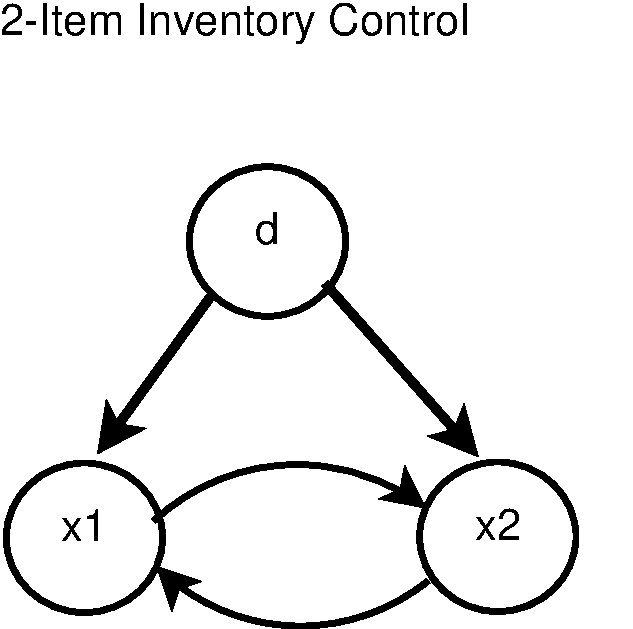
\includegraphics[width=0.2\textwidth]{Figures1/diagrams/dbn_state.pdf}
        \end{subfigure}
                \hspace{2mm}
\begin{subfigure}
                \centering
                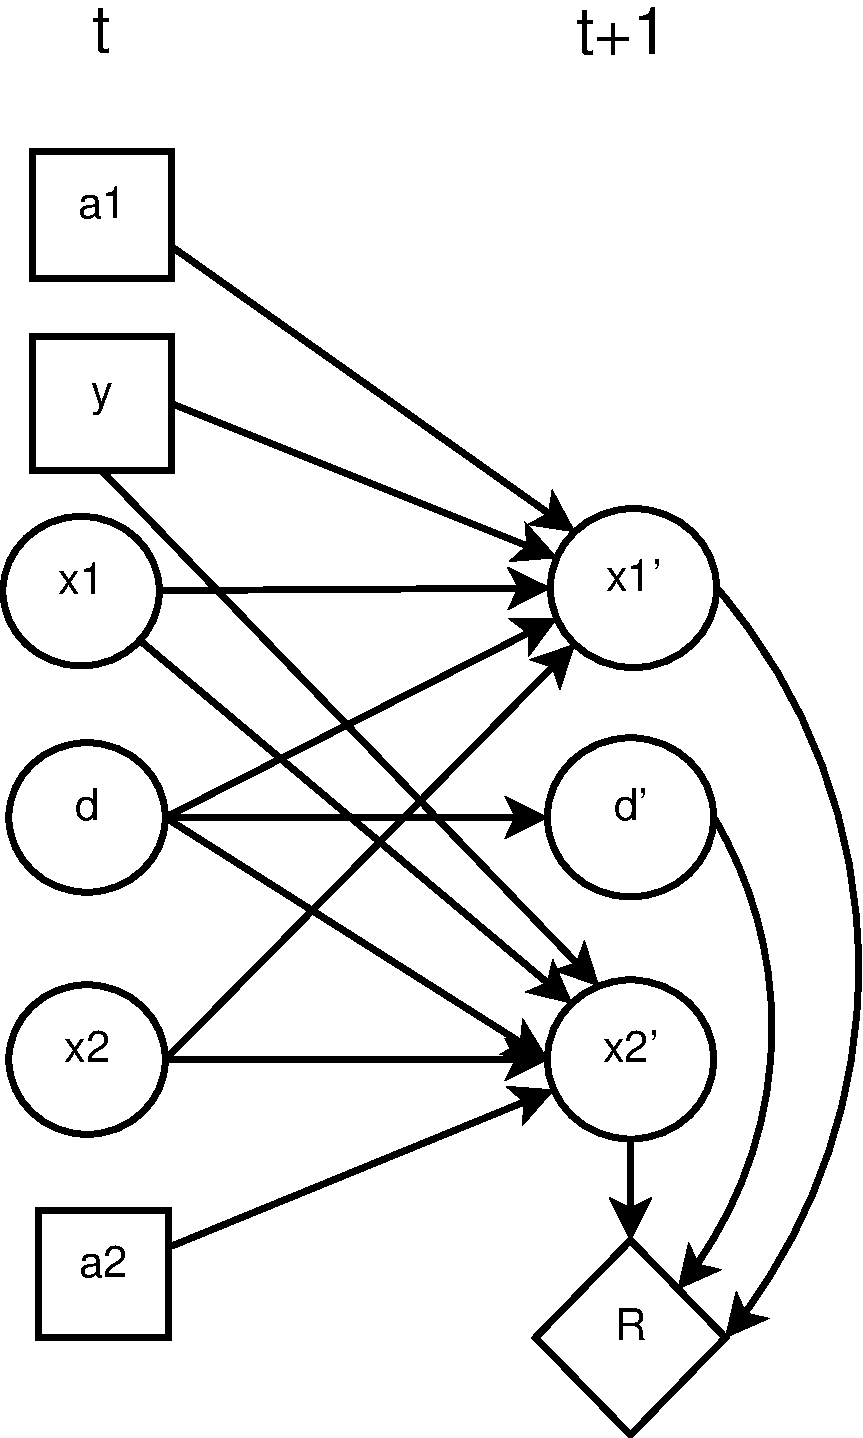
\includegraphics[width=0.25\textwidth]{Figures1/diagrams/dbn_inv2.pdf}
        \end{subfigure}
                        \hspace{-1mm}
\begin{subfigure}
                \centering
                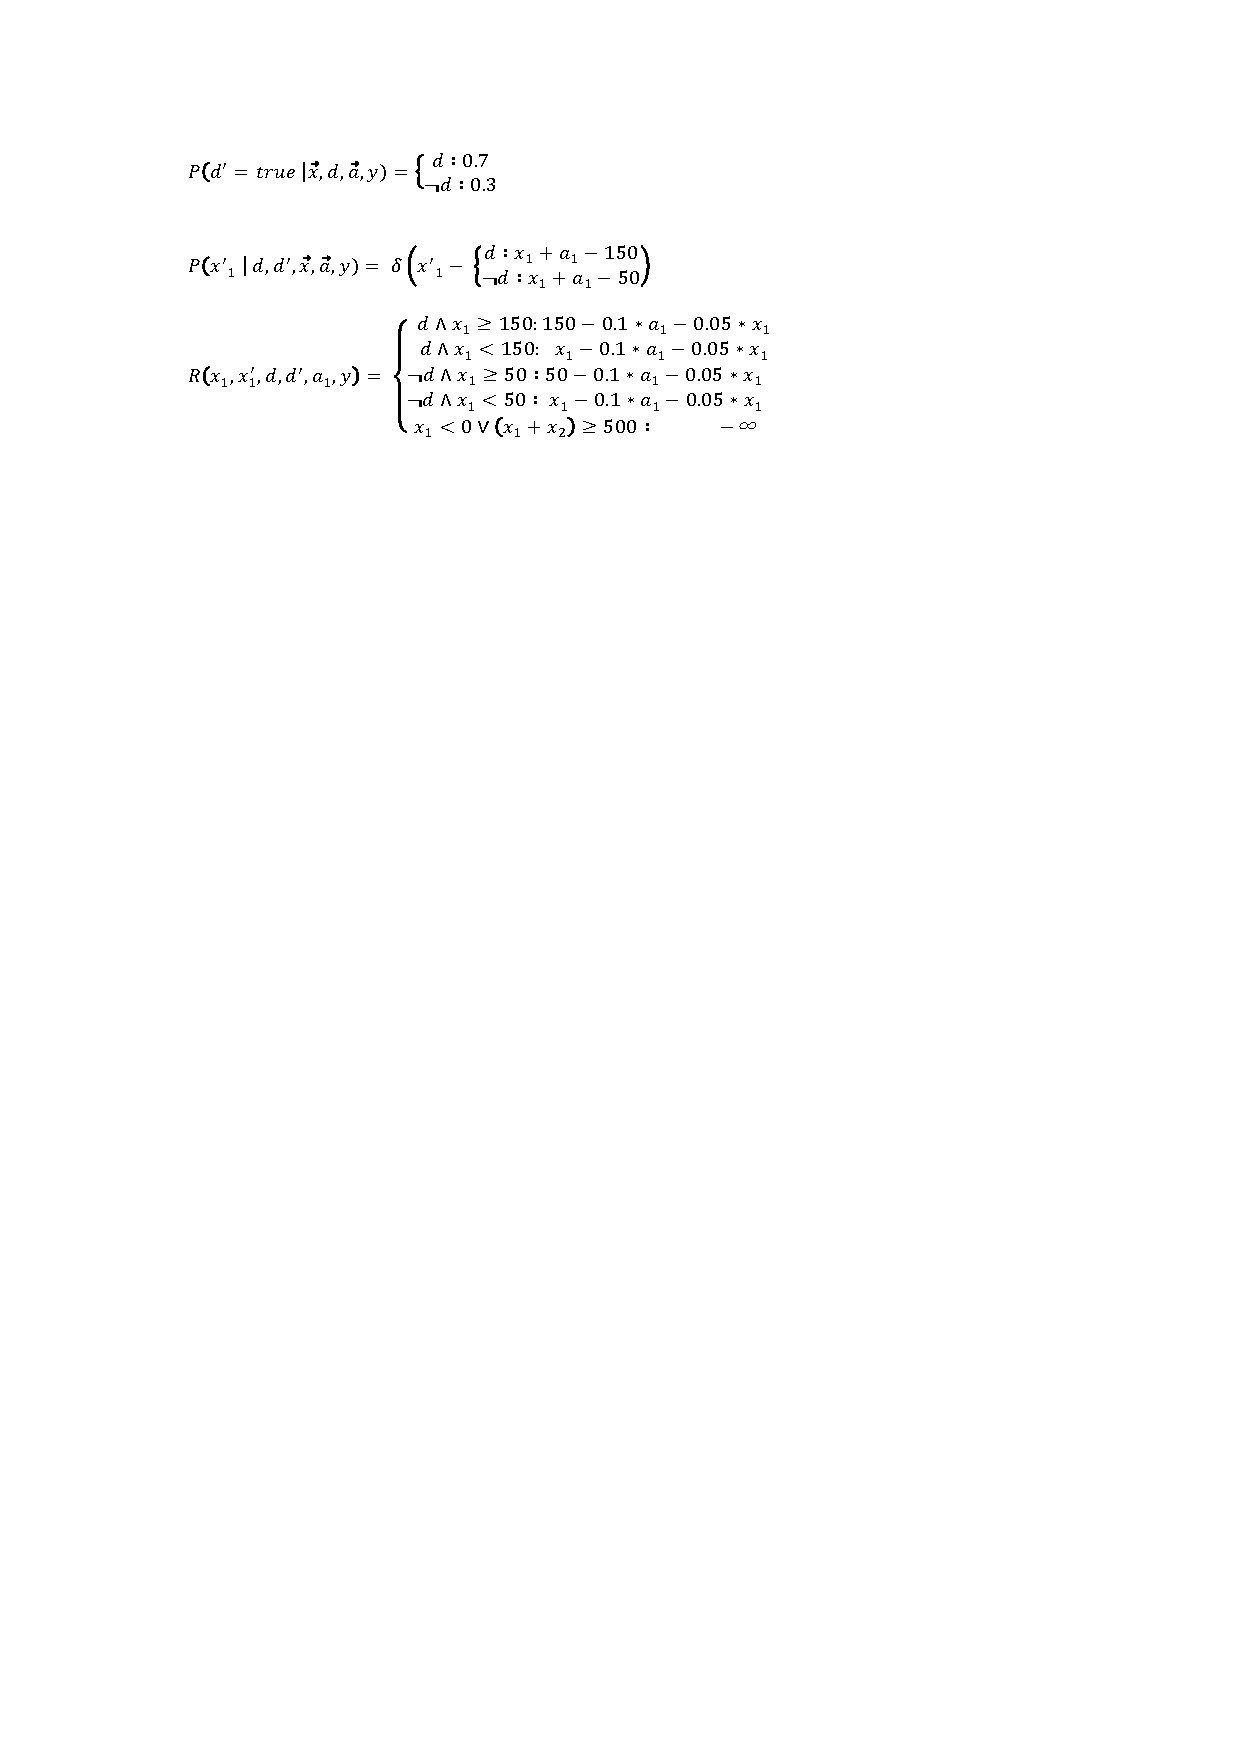
\includegraphics[width=0.55\textwidth]{Figures2/diagrams/probabilities_2.pdf}
        \end{subfigure}
        \vspace{-3mm}
\caption{\footnotesize Network topology between state variables in the 2-item continuous action \InventoryControl (CAIC) problem (Left); Dynamic bayes network (DBN) structure representing the transition and reward function (Middle); transition probabilities and reward function in terms of CPF and PLE for $x_1$ (Right). }
\label{fig:dbn}
\vspace{-3mm}
\end{figure}
%%%%%%%%%%%%%%%%%%%%%%%%%%%%%%%%%%%%%%%%%%%%%%%%%%%%%%%%%%%%%%%%%%%%%%%%%%

Such HMDPs are naturally factored \cite{boutilier99dt}
in terms of state variables $(\vec{b},\vec{x},\vec{y})$ where potentially $\vec{y} =0$. The transition structure can be exploited in the form of a dynamic Bayes
net (DBN) \cite{dbn} where the conditional probabilities
$P(b_i'|\cdots)$ and $P(x_j'|\cdots)$ for each next state variable can
condition on the action, current and next state. 
We can also have \emph{synchronic arcs} (variables that condition on each
other in the same time slice) within the binary $\vec{b}$ or
continuous variables $\vec{x}$ and from $\vec{b}$ to $\vec{x}$.%\footnote{Synchronic arcs between variables within $\vec{b}$ or within $\vec{x}$ can be accommodated if the forthcoming Algorithm~\ref{alg:regress} (\texttt{Regress}) is modified to multiply and marginalize-out multiple next-state variables in one elimination step according to the DBN structure.}  
Hence we can factorize the joint transition model as
{%\footnotesize
\begin{equation}
P(\vec{b}',\vec{x}'|\vec{b},\vec{x},a,\vec{y}) = 
\prod_{i=1}^n P(b_i'|\vec{b},\vec{x},\vec{b'},\vec{x'},a,\vec{y}) \prod_{j=1}^m P(x_j'|\vec{b},\vec{b}',\vec{x},\vec{x'},a,\vec{y}). \nonumber %\label{eq:dbn} 
\end{equation}}
where $P(b_i'|\vec{b},\vec{x},\vec{b'},\vec{x'},a,\vec{y})$ may condition on a subset of
$\vec{b}$ and $\vec{x}$ in the current and next state and likewise 
$P(x_j'|\vec{b},\vec{b}',\vec{x},\vec{x'},a,\vec{y})$ may condition on a subset of
$\vec{b}$, $\vec{b}'$, $\vec{x}$ and $\vec{x'}$. Figure ~\ref{fig:dbn} presents the DBN for our CAIC example according to this definition.  

We call the conditional probabilities
$P(b_i'|\vec{b},\vec{x},\vec{b'},\vec{x'},a,\vec{y})$ for \emph{binary} variables $b_i$
($1 \leq i \leq n$) conditional probability functions (CPFs) --- not
tabular enumerations --- because in general these functions can
condition on both discrete and continuous state as
in the right-hand side of ~\eqref{eq:trans_inv}.  For the \emph{continuous} variables
$x_j$ ($1 \leq j \leq m$), we represent the CPFs
$P(x_j'|\vec{b},\vec{b'},\vec{x},\vec{x'},a,\vec{y})$ with \emph{piecewise
linear equations} (PLEs) satisfying three properties: 

(i) PLEs can only condition on the
action, current state, and previous state variables

(ii) PLEs are deterministic meaning that to be represented by probabilities they
must be encoded using Dirac $\delta[\cdot]$ functions (example forthcoming)

(iii) PLEs are piecewise linear, where the piecewise conditions may be arbitrary logical combinations of $\vec{b}$, $\vec{b}'$ 
and linear inequalities over $\vec{x}$ and $\vec{x'}$.  

The transition function example provided in the left-hand side of ~\eqref{eq:trans_inv} can be expressed in PLE format such as the right figure in Figure ~\ref{fig:dbn}.
The use of the $\delta[\cdot]$ function ensures that the PLEs are conditional
probability functions that integrates to 1 over $x'_j$; In more intuitive
terms, one can see that this $\delta[\cdot]$ is a simple way to encode
the PLE transition $x' = \left\{ \ldots \right.$ in the form of 
$P(x_j'|\vec{b},\vec{b'},\vec{x},\vec{x'},a,\vec{y})$.

%qualify the extent of stochasticity and other restrictions
While it will be clear that our restrictions do not permit general stochastic transition noise (e.g., Gaussian noise as in LQG control), they do permit discrete noise in the sense that
$P(x_j'|\vec{b},\vec{b'},\vec{x},\vec{x'},a,\vec{y})$ may condition on
$\vec{b'}$, which are stochastically sampled according to their CPFs.
\footnote{Continuous stochastic noise for the transition function is an on going work which allows us to model stochasticity more generally}
We note that this representation effectively allows modeling of
continuous variable transitions as a mixture of $\delta$ functions,
which has been used frequently in previous exact continuous state MDP
solutions \cite{feng04,hao09}.
% should I put this????
Furthermore, we note that our
representation is more general in DA-HMDPs than \cite{feng04,li05,hao09} in that
we do not restrict the equation to be linear, but rather
allow it to specify \emph{arbitrary} functions (e.g., nonlinear). The reward function can also be defined as \emph{arbitrary} function of the current state for each action $a \in A$. 
While our DA-HMDP examples throughout the paper will demonstrate the full expressiveness of our symbolic dynamic programming approach, we note that there are computational advantages to be had when the reward and transition case conditions and functions can be restricted to linear polynomials.  

Due to the same restrictions for CA-HMDPs the reward function $R(\vec{b},\vec{b'},\vec{x},\vec{x'}, a,\vec{y})$ is defined as either of the following:

(i) a general piecewise linear function (boolean or linear conditions and linear values) such as ~\eqref{rew_inv}  

(ii) a piecewise quadratic function of univariate state and a linear function of univariate action parameters:
\begin{align}
R(x,x',d,d', a) & = \begin{cases}
\neg d \land x \geq -2 \land x \leq 2 : & 4 - x^2 \\
d \lor x < -2 \lor x > 2 : & 0
\end{cases} \label{rew:nonlinear}
\end{align}
%The reward function in a DA-HMDPs can potentially be defined as an \emph{arbitrary} function but to ensure computationally efficient results we assume piecewise linear boundaries that can be checked for consistency using a linear constraint feasibility checker, which we will later see is crucial for efficiency.

These transition and reward constraints will ensure that all derived functions in the solution of HMDPs adhere to the reward 
constraints.

%\vspace*{-0.05in}
\subsection{Solution methods}
\label{sec:soln}
Now we provide a continuous state generalization of {\it value
iteration} \cite{bellman}, which is a dynamic programming algorithm
for constructing optimal policies.  It proceeds by constructing a
series of $h$-stage-to-go value functions $V^h(\vec{b},\vec{x})$.
Initializing $V^0(\vec{b},\vec{x}) = 0$ we define the quality
$Q_a^{h}(\vec{b},\vec{x},\vec{y})$ of taking action $a(\vec{y})$ in state
$(\vec{b},\vec{x})$ and acting so as to obtain
$V^{h-1}(\vec{b},\vec{x})$ thereafter as the following:

\vspace{-4mm}
{%\footnotesize
\begin{align}
Q_a^{h}(\vec{b},\vec{x},\vec{y}) & = 
 \sum_{\vec{b}'} \hspace{-1.0mm} \int \hspace{-1.0mm} \left( \prod_{i=1}^n P(b_i'|\vec{b},\vec{x},\vec{b'},\vec{x'},a,\vec{y}) \prod_{j=1}^m P(x_j'|\vec{b},\vec{b}',\vec{x},\vec{x'},a,\vec{y}) \right) \label{eq:qfun} \\ 
& \Bigg[ R(\vec{b},\vec{b'},\vec{x},\vec{x'}, a,\vec{y}) + \gamma \cdot V^{h-1}(\vec{b}',\vec{x}') d\vec{x}'  \hspace{-0.2mm} \Bigg] \nonumber
\end{align}}
Given $Q_a^h(\vec{b},\vec{x},\vec{y})$ for each $a \in A$ where $\vec{y}$ can also be empty , we can proceed
to define the $h$-stage-to-go value function as follows:
\begin{align}
V^{h}(\vec{b},\vec{x}) & = \max_{a \in A} \max_{\vec{y} \in \mathbb{R}^{|\vec{y}|}} \left\{ Q^{h}_a(\vec{b},\vec{x},\vec{y}) \right\} \label{eq:vfun}
\end{align}

For discrete actions, maximization over the continuous parameter $\vec{y}$ is omitted. The $max_{\vec{y}}$ operator will be defined in the next section and is required to generalize solutions from DA-HMDPs to CA-HMDPs.
If the horizon $H$ is finite, then the optimal value function is
obtained by computing $V^H(\vec{b},\vec{x})$ and the optimal
horizon-dependent policy $\pi^{*,h}$ at each stage $h$ can be easily
determined via $\pi^{*,h}(\vec{b},\vec{x}) = \argmax_a
\argmax_{\vec{y}} Q^h_a(\vec{b},\vec{x},\vec{y})$.  If the horizon $H
= \infty$ and the optimal policy has finitely bounded value, then
value iteration can terminate at horizon $h$ if $V^{h} = V^{h-1}$;
then $V^\infty = V^h$ and $\pi^{*,\infty} = \pi^{*,h}$.

In DA-HMDPs, we can always compute the value function in tabular form;
however, how to compute this for HMDPs with reward and transition
function as previously defined is the objective of the symbolic
dynamic programming algorithm that we define in the next section.
From this \emph{mathematical} definition, we  
show how to \emph{compute}~\eqref{eq:qfun} and \eqref{eq:vfun} 
for the previously defined HMDPs.

\section{Symbolic Dynamic Programming} \label{SDP}
%\vspace*{-0.05in}
As it's name suggests, symbolic dynamic programming (SDP) \cite{fomdp}
is simply the process of performing dynamic programming (in this case
value iteration) via symbolic manipulation.  While SDP as defined
in \cite{fomdp} was previously only used with piecewise
constant functions, we now generalize the representation to work with
general piecewise functions for HMDPs in this article.  
%Should all this be taken out?
%We present the general SDP framework for value iteration in DA-HMDPs in Algorithm~\ref{alg:vi} (\texttt{VI}). Further we define  Algorithm~\ref{alg:contMax}(\texttt{Continuous Maximization}) to deal with the final maximization in (~\ref{eq:vfun}) for continuous actions.

Before we define our solution, however, we must formally define our
case representation and symbolic case operators.

\subsection{Case Representation and Operations}
%\vspace*{-0.05in}
Throughout this article, we will assume that all symbolic functions
can be represented in \emph{case} form as follows:
{%\footnotesize 
\begin{align*}
f = 
\begin{cases}
  \phi_1: & f_1 \\ 
 \vdots&\vdots\\ 
  \phi_k: & f_k \\ 
\end{cases}
\end{align*}
}
Here the $\phi_i$ are logical formulae defined over the state
$(\vec{b},\vec{x})$ that can include arbitrary logical ($\land,\lor,\neg$)
combinations of (a) boolean variables in $\vec{b}$ and (b) 
inequalities ($\geq,>,\leq,<$), equalities ($=$), or disequalities ($\neq$)
where the left and right operands can be \emph{any} function of one or more 
variables in $\vec{x}$.  
Each $\phi_i$ will be disjoint from the other $\phi_j$ ($j \neq i$); 
however the $\phi_i$ may not exhaustively cover the state space, hence
$f$ may only be a \emph{partial function} and may be undefined for some
state assignments. In general we require $f$ to be continuous (including no discontinuities at partition boundaries); operations preserve this property. The main operations required to perform SDP are provided below in the case calculus: 
\subsubsection*{Scalar multiplication and Negation}
\emph{Unary operations} such as scalar multiplication $c\cdot f$ (for
some constant $c \in \mathbb{R}$) or negation $-f$ on case statements
$f$ are presented below; the unary operation is simply applied to each
$f_i$ ($1 \leq i \leq k$). 
{%\footnotesize
\begin{center}
\begin{tabular}{r c c l}
&
%\hspace{5mm}
  $c \cdot f = \begin{cases}
    \phi_1  : & c \cdot f_1 \\ 
   \vdots&\vdots\\ 
    \phi_k : & c \cdot f_k \\ 
  \end{cases}$
 &
\vspace{10mm}
  $-f = \begin{cases}
    \neg \phi_1 : & f_1 \\ 
   \vdots&\vdots\\ 
    \neg \phi_k : & f_k \\ 
  \end{cases}$
\end{tabular}
\end{center}
}
\vspace{-9mm} 
\subsubsection*{Binary operations}
Intuitively, to perform a \emph{binary
 operation} on two case statements, we simply take the cross-product
of the logical partitions of each case statement and perform the
corresponding operation on the resulting paired partitions.  Letting
each $\phi_i$ and $\psi_j$ denote generic first-order formulae, we can
perform the ``cross-sum'' $\oplus$ and ``cross-product'' $\otimes$ of two (unnamed) cases in the
following manner:

{\footnotesize 
\begin{center}
\begin{tabular}{r c c c l}
&
\hspace{-6mm} 
  $\begin{cases}
    \phi_1: & f_1 \\ 
    \phi_2: & f_2 \\ 
  \end{cases}$
$\oplus$
&
\hspace{-4mm}
  $\begin{cases}
    \psi_1: & g_1 \\ 
    \psi_2: & g_2 \\ 
  \end{cases}$
&
\hspace{-2mm} 
$ = $
&
\hspace{-2mm}
  $\begin{cases}
  \phi_1 \wedge \psi_1: & f_1 + g_1 \\ 
  \phi_1 \wedge \psi_2: & f_1 + g_2 \\ 
  \phi_2 \wedge \psi_1: & f_2 + g_1 \\ 
  \phi_2 \wedge \psi_2: & f_2 + g_2 \\ 
  \end{cases}$
\end{tabular}
\vspace{4mm}
\hspace{-2mm}
\begin{tabular}{r c c c l}
&
\hspace{-6mm} 
  $\begin{cases}
    \phi_1: & f_1 \\ 
    \phi_2: & f_2 \\ 
  \end{cases}$
$\otimes$
&
\hspace{-4mm}
  $\begin{cases}
    \psi_1: & g_1 \\ 
    \psi_2: & g_2 \\ 
  \end{cases}$
&
\hspace{-2mm} 
$ = $
&
\hspace{-2mm}
  $\begin{cases}
  \phi_1 \wedge \psi_1: & f_1 * g_1 \\ 
  \phi_1 \wedge \psi_2: & f_1 * g_2 \\ 
  \phi_2 \wedge \psi_1: & f_2 * g_1 \\ 
  \phi_2 \wedge \psi_2: & f_2 * g_2 \\ 
  \end{cases}$
\end{tabular}
\end{center}
}
\normalsize
Likewise, we can perform $\ominus$ by subtracting partition values to obtain the result.  Some partitions resulting from
the application of the $\oplus$, $\ominus$, and $\otimes$ operators
may be inconsistent (infeasible); we may simply discard such 
partitions as they are irrelevant to the function value.

\subsubsection*{Symbolic maximization}
For SDP, we'll also need to perform which is fairly straightforward
to define:
%\vspace{-5mm}

{%\footnotesize
\begin{center}
\begin{tabular}{r c c c l}
&
\hspace{-9mm} $\casemax \Bigg(
  \begin{cases}
    \phi_1: & f_1 \\ 
    \phi_2: & f_2 \\ 
  \end{cases}$
$,$
&
\hspace{-4mm}
  $\begin{cases}
    \psi_1: & g_1 \\ 
    \psi_2: & g_2 \\ 
  \end{cases} \Bigg)$
&
\hspace{-4mm} 
$ = $
&
\hspace{-4mm}
  $\begin{cases}
  \phi_1 \wedge \psi_1 \wedge f_1 > g_1    : & f_1 \\ 
  \phi_1 \wedge \psi_1 \wedge f_1 \leq g_1 : & g_1 \\ 
  \phi_1 \wedge \psi_2 \wedge f_1 > g_2    : & f_1 \\ 
  \phi_1 \wedge \psi_2 \wedge f_1 \leq g_2 : & g_2 \\ 
  \phi_2 \wedge \psi_1 \wedge f_2 > g_1    : & f_2 \\ 
  \phi_2 \wedge \psi_1 \wedge f_2 \leq g_1 : & g_1 \\ 
  \phi_2 \wedge \psi_2 \wedge f_2 > g_2    : & f_2 \\ 
  \phi_2 \wedge \psi_2 \wedge f_2 \leq g_2 : & g_2 \\ 
  \end{cases}$
\end{tabular}
\end{center}
}
One can verify that the resulting case statement is still
within the case language defined previously.  At first
glance this may seem like a cheat and little is gained
by this symbolic sleight of hand.  However, simply
having a case partition representation that is closed under 
maximization will facilitate the closed-form regression 
step that we need for SDP.\ \  Furthermore, the 
XADD that we introduce later will be able to exploit the 
internal decision structure of this
maximization to represent it much more compactly.

\subsubsection*{Restriction}
In the next operation of \emph{restriction} %is fairly simple: in this operation, 
we want to restrict a function $f$ to apply only in cases
that satisfy some formula $\phi$, which we write as $f|_{\phi}$.  
This can be done by simply appending $\phi$ to each case partition
as follows:

{%\footnotesize
\begin{center}
\begin{tabular}{r c c l}
&
\hspace{-6mm} 
  $f = \begin{cases}
    \phi_1: & f_1 \\ 
   \vdots&\vdots\\ 
    \phi_k: & f_k \\ 
  \end{cases}$
&

&
\hspace{-2mm}
  $f|_{\phi} = \begin{cases}
    \phi_1 \land \phi : & f_1 \\ 
   \vdots&\vdots\\ 
    \phi_k \land \phi : & f_k \\ 
  \end{cases}$
\end{tabular}
\end{center}
}
Clearly $f|_{\phi}$ only applies when $\phi$ holds and is
undefined otherwise, hence $f|_{\phi}$ is a partial function
unless $\phi \equiv \top$.

\subsubsection*{Substitution}
\emph{Symbolic substitution} simply takes
a set $\sigma$ of variables and their substitutions, e.g., 
$\sigma = \{ x_1' / (x_1 \hspace{-.8mm} + \hspace{-.8mm} x_2), x_2' / x_1^2 \hspace{-.3mm} \exp(x_2) \}$ where
the LHS of the $/$ represents the substitution variable and the
RHS of the $/$ represents 
the expression that should be substituted in its place.  No variable
occurring in any RHS expression of $\sigma$ can also occur in any 
LHS expression of $\sigma$.
We write the substitution of a non-case function $f_i$ with $\sigma$ 
as $f_i\sigma$; as an example, for the $\sigma$ defined previously and 
$f_i = x_1' + x_2'$ then $f_i\sigma = x_1 + x_2 + x_1^2 \exp(x_2)$ as
would be expected.  We can also substitute into case partitions $\phi_j$
by applying $\sigma$ to each inequality operand; as an example, if
$\phi_j \equiv x_1' \leq \exp(x_2')$ then 
$\phi_j \sigma \equiv x_1 + x_2 \leq \exp(x_1^2 \exp(x_2))$.
Having now defined substitution of $\sigma$ for non-case functions $f_i$ and case
partitions $\phi_j$ we can define it for case statements in general:

{%\footnotesize
\begin{center}
\begin{tabular}{r c c l}
&
\hspace{-6mm} 
  $f = \begin{cases}
    \phi_1: & f_1 \\ 
   \vdots&\vdots\\ 
    \phi_k: & f_k \\ 
  \end{cases}$
&

&
\hspace{-2mm}
  $f\sigma = \begin{cases}
    \phi_1\sigma: & f_1\sigma \\ 
   \vdots&\vdots\\ 
    \phi_k\sigma: & f_k\sigma \\ 
  \end{cases}$
\end{tabular}
\end{center}
}
\normalsize

One property of substitution is that
if $f$ has mutually exclusive partitions $\phi_i$ ($1 \leq i \leq k$)
then $f\sigma$ must also have mutually exclusive partitions ---
this follows from the logical consequence that 
if $\phi_1 \land \phi_2 \models \bot$
then $\phi_1\sigma \land \phi_2\sigma \models \bot$.
%We will exploit this property next in SDP for HMDPs.

\subsubsection*{Continuous Integration of the $\delta$-function}
\emph{Continuous Integration} evaluates the integral
marginalization $\int_{\vec{x}}$ over the continuous variables
in a function $f$. One of the \emph{key novel insights of SDP} in the context of
HMDPs is that the integration 
$\int_{x_j'} \delta[x_j' - g(\vec{x})] f dx_j'$ 
simply \emph{triggers the substitution} $\sigma = \{ x_j' / g(\vec{x}) \}$
on $f$, that is
\begin{align}
\int_{x} \delta[x - g(\vec{x})] f dx' \; = \; f \{x / g(\vec{x}) \} . \label{eq:gen_int}
\end{align}

To perform ~\ref{eq:gen_int} on a more general
representation, we obtain: 
\begin{align*}
    = \begin{cases}
    \phi_1: & f \{ x = g_1 \} \\ 
   \vdots&\vdots\\ 
    \phi_k: & f \{ x= g_k \}  \\ 
  \end{cases}
\end{align*}

 Here we note that because $f$ is \emph{already} a case
statement, we can simply replace the single partition $\phi_i$ with the
multiple partitions of $f\{ x / g_i \}|_{\phi_i}$.%\footnote{If $V'^h$
%had mutually disjoint partitions then we note the restriction and
%substitution operations preserve this disjointness.}  
This reduces the \emph{nested} case statement back down to a non-nested case
statement as in the following example:
\begin{align*}
    \begin{cases}
      \phi_1: & 
        \begin{cases}
          \psi_1: & f_{11} \\ 
          \psi_2: & f_{12}  \\ 
        \end{cases} \\
      \phi_2: & 
        \begin{cases}
          \psi_1: & f_{21} \\ 
          \psi_2: & f_{22}  \\ 
        \end{cases} \\
    \end{cases} & \; = \;
        \begin{cases}
          \phi_1 \land \psi_1: & f_{11} \\ 
          \phi_1 \land \psi_2: & f_{12}  \\ 
          \phi_2 \land \psi_1: & f_{21} \\ 
          \phi_2 \land \psi_2: & f_{22}  \\ 
        \end{cases} 
\end{align*}

\subsubsection*{Continuous Maximization}
\emph{Continuous Maximization} of a variable $y$ is defined as $g(\vec{b},\vec{x}) := \max_{\vec{y}}
\, f(\vec{b},\vec{x},\vec{y})$ where we crucially note that 
\emph{the} maximizing $\vec{y}$ is a function
$g(\vec{b},\vec{x})$, hence requiring \emph{symbolic} 
constrained optimization. We can rewrite $f(\vec{b},\vec{x},y)$ via 
the following equalities:
\footnote{The second line ensures that all illegal values are mapped to $-\infty$}
{%\footnotesize
\begin{align}
\max_y f(\vec{b},\vec{x},y) & = 
\max_y \casemax_i \, \phi_i(\vec{b},\vec{x},y) f_i(\vec{b},\vec{x},y) \nonumber \\
& = \casemax_i \, \fbox{$\max_y \phi_i(\vec{b},\vec{x},y) f_i(\vec{b},\vec{x},y)$} \label{eq:casemax_max}
\end{align}
}
Because the 
$\phi_i$ are mutually disjoint and exhaustive, 
$f(\vec{b},\vec{x},y) = \casemax_i \, \phi_i(\vec{b},\vec{x},y) f_i(\vec{b},\vec{x},y)$.  
%The first equality is a consequence of the mutual  disjointness of the partitions in $f$.  
Then because 
$\max_y$ and $\casemax_i$ are commutative and may be reordered,
we can compute $\max_y$ for \emph{each case partition
individually}.  Thus to complete this section we need only
show how to symbolically compute a single partition 
$\max_y \phi_i(\vec{b},\vec{x},y): f_i(\vec{b},\vec{x},y)$.

In $\phi_i$, we observe that each conjoined constraint serves one of
three purposes: 

(i) \emph{upper bound on $y$}: it can be written
as $y < \cdots$ or $y \leq \cdots$.

(ii) \emph{lower bound on $y$}: it can be written as $y >
\cdots$ or $y \geq \cdots$.
\footnote{For purposes of evaluating
a case function $f$ at an upper or lower bound,
it does not matter whether a bound is inclusive ($\leq$ or $\geq$)
or exclusive ($<$ or $>$) since $f$ is required to be continuous
and hence evaluating at the limit of the inclusive bound will
match the evaluation for the exclusive bound.}

(iii) \emph{independent of $y$}: the constraints do not contain $y$
and can be safely factored outside of the $\max_y$.

Because there are multiple symbolic upper and lower
bounds on $y$, in general we will need to apply the $\casemax$
($\casemin$) operator to determine the highest lower bound $\LB$
(lowest upper bound $\UB$).

We also know that $\max_y \phi_i(\vec{b},\vec{x},y)
f_i(\vec{b},\vec{x},y)$ for a continuous function $f_i$ must occur at the critical points of the function --- 
either the upper or lower bounds ($\UB$ and $\LB$) of $y$, 
or the $\Root$ (i.e., zero) of $\frac{\partial}{\partial y} f_i$ 
w.r.t.\ $y$.  Each of $\UB$, $\LB$, and $\Root$
is a symbolic function of $\vec{b}$ and $\vec{x}$. 

Given the \emph{potential} maxima points of $y = \UB$, $y = \LB$, and
$y = \Root$ of $\frac{\partial}{\partial y} f_i(\vec{b},\vec{x},y)$
w.r.t. constraints $\phi_i(\vec{b},\vec{x},y)$ --- which are all
symbolic functions --- we must symbolically evaluate which yields the
maximizing value $\Max$ for this case partition:
\vspace{2mm}
{%\footnotesize
\begin{align*}
\Max =  \sq \begin{cases}
\mbox{$\exists \Root$}  \sq: \sq & \sqm \casemax( f_i \{ y / \Root \}, f_i \{ y / \UB \}, f_i \{ y / \LB \})\\
\mbox{else}  \sq:  \sq & \sqm \casemax( f_i \{ y / \UB \}, f_i \{ y / \LB \})
\end{cases}
\end{align*}}
Here $\casemax(f,g,h) = \casemax(f,\casemax(g,h))$.  The 
substitution operator $\{ y / f \}$ replaces $y$ with case statement $f$, 
defined previously.

At this point, we have almost completed the computation
of the $\max_y \phi_i(\vec{b},\vec{x},y) f_i(\vec{b},\vec{x},y)$
except for one issue: the incorporation of the independent ($\IND$) constraints
(factored out previously) and additional constraints that arise from the
symbolic nature of the $\UB$, $\LB$, and $\Root$.  

Specifically for the latter, we need to ensure that indeed $\LB \leq \Root \leq \UB$
(or if no root exists, then $\LB \leq \UB$) by building a set
of constraints $\CONS$ that ensure these conditions hold; to do this,
it suffices to ensure that for each possible expression $e$ used to
construct $\LB$ that $e \leq \Root$ and similarly for the $Root$ and $\UB$.
Now we express the final result as a single case partition:
\begin{equation*}
\max_y \phi_i(\vec{b},\vec{x},y) f_i(\vec{b},\vec{x},y) \;\; = \;\;
\left\{ \CONS \land \IND: \Max \right.
\end{equation*}
Hence, to complete the maximization for an entire case statement $f$, we need only apply the above procedure to each case partition of $f$ and then  perform a symbolic $\casemax$ all of these results.  

\subsection{Symbolic Dynamic Programming (SDP)}

In this section we present the Symbolic value iteration algorithm (SVI) for HMDPs.

%%%%%%%%%%%%%%%%%%%%%%%%%%%%%%%%%%%%%%%%%%%%%%%%%%%%%%%%%%%%%%%%%%%%%%%%
\incmargin{.5em}
\linesnumbered
\begin{algorithm}[t!]
\vspace{-.5mm}
\dontprintsemicolon
\SetKwFunction{regress}{Regress}
\Begin
{
   $V^0:=0, h:=0$\;
   \While{$h < H$}
   {
       $h:=h+1$\;
       \ForEach {$a(\vec{y}) \in A$}
       {
              $Q_a^{h}(\vec{y})\,:=\,$\regress{$V^{h-1},a,\vec{y}$}\;
			  \emph{//Continuous action parameter}\;
			  \If  {$ \mid \vec{y} \mid >0$}  
               {
               $Q_a^{h}(\vec{y}) := \max_{\vec{y}} \, Q_a^{h}(\vec{y})$ $\,$ \;
               $\pi^{*,h} := \argmax_{a} \, Q_a^{h}(\vec{y})$\;
               } 
               \Else 
               { $\pi^{*,h} := \argmax_{a} \, Q_a^{h}(\vec{y})$ \; }
        }
       $V^{h} := \casemax \, Q_a^{h}(\vec{y})$ $\,$ \;
       \If{$V^h = V^{h-1}$}
           {break $\,$ \emph{// Terminate if early convergence}\;}
   }
     \Return{$(V^h,\pi^{*,h})$} \;
}
\caption{\footnotesize \texttt{VI}(HMDP, $H$) $\longrightarrow$ $(V^h,\pi^{*,h})$ \label{alg:vi}}
\vspace{-1mm}
\end{algorithm}
\decmargin{.5em}
%%%%%%%%%%%%%%%%%%%%%%%%%%%%%%%%%%%%%%%%%%%%%%%%%%%%%%%%%%%%%%%%%

%%%%%%%%%%%%%%%%%%%%%%%%%%%%%%%%%%%%%%%%%%%%%%%%%%%%%%%%%%%%%%%%%
\incmargin{.5em}
\linesnumbered
\begin{algorithm}[t!]
\vspace{-.5mm}
\dontprintsemicolon
\SetKwFunction{remapWithPrimes}{Prime}
%\SetKwFunction{sumout}{sumout}


\Begin{
    $Q=$ \remapWithPrimes{$V$} $\,$ \emph{// All $b_i \to b_i'$ and all $ x_i \to x_i'$} \;
%    \emph{// Continuous regression marginal integration}\\
%    \For {all $x'_j$ in $Q$}{
%         $Q := \int Q \otimes P(x_j'|\vec{b},\vec{b}',\vec{x},a,\vec{y}) \, d_{x'_j}$\;
%    }
%    \emph{// Discrete regression marginal summation}\\
%    \For {all $b'_i$ in $Q$}{
%         $Q := \left[ Q \otimes P(b_i'|\vec{b},\vec{x},a,\vec{y}) \right]|_{b_i' = 1}$\\
%         \hspace{8mm} $\oplus \left[ Q \otimes P(b_i'|\vec{b},\vec{x},a,\vec{y}) \right]|_{b_i' = 0}$\;
%    }
%    \Return{$R(\vec{b},\vec{x},a,\vec{y}) \oplus (\gamma \otimes Q)$} \;
\If {$v'$ in $R$}
	 {$Q := R(\vec{b},\vec{b}',\vec{x},\vec{x}',a,\vec{y}) \oplus (\gamma \cdot Q)$} \;
    \ForEach { $v'$ in $Q$}  
    {
    	\If {$v'$ = $x'_j$}
    	{
    	\emph{//Continuous marginal integration}\\
         $Q := \int Q \otimes P(x_j'|\vec{b},\vec{b}',\vec{x},\vec{x}',a,\vec{y}) \, d_{x'_j}$\;
    	}
	    \If {$v'$=$b'_i$}
    	{
    	\emph{// Discrete marginal summation}\\
         $Q := \left[ Q \otimes P(b_i'|\vec{b},\vec{b}',\vec{x},\vec{x}',a,\vec{y}) \right]|_{b_i' = 1}$
         $\oplus \left[ Q \otimes P(b_i'|\vec{b},\vec{b},\vec{x},\vec{x}',a,\vec{y}) \right]|_{b_i' = 0}$\;
    	}
    }
    \If {$\neg$ ($v'$  in $R$)}
    {$Q := R(\vec{b},\vec{b}',\vec{x},\vec{x}',a,\vec{y}) \oplus (\gamma \cdot Q)$ }\;
    \Return{$Q$} \;
}
\caption{\footnotesize \texttt{Regress}($V,a,\vec{y}$) $\longrightarrow$ $Q$ \label{alg:regress}}
\vspace{-1mm}
\end{algorithm}
\decmargin{.5em}
%%%%%%%%%%%%%%%%%%%%%%%%%%%%%%%%%%%%%%%%%%%%%%%%%%%%%%%%%%%%%%%%%

Our objective is to take a DA-HMDP or CA-HMDP as defined in Section~\ref{sec:HMDPs}, apply value
iteration as defined in Section~\ref{sec:soln}, and produce
the final value optimal function $V^h$ at horizon $h$ in the form
of a case statement. Algorithm ~\ref{alg:vi} presents this briefly. 

For the base case of $h=0$ in line 2, we note that setting $V^0(\vec{b},\vec{x}) = 0$
(or to the reward case statement, if not action dependent)
%and $R(\vec{b},\vec{x})$ as described in Section~\ref{sec:HMDPs}
is trivially in the form of a case statement.

Next, for $h > 0$ and for each action in line 5 we must perform lines 6--12. Starting with the application of Algorithm~\ref{alg:regress}.  Note that we have omitted parameters $\vec{b}$ and
$\vec{x}$ from $V$ and $Q$ to avoid notational clutter.
Fortunately, given our previously defined
operations, SDP is straightforward and can be divided into five 
steps: 
\begin{enumerate}
\item {\it Prime the Value Function}: Since $V^{h}$ will become
the ``next state'' in value iteration, we setup a substitution
$\sigma = \{ b_1 / b_1', \ldots, b_n / b_n', x_1 / x_1', \ldots, x_m / x_m' \}$
and obtain $V'^{h} = V^{h}\sigma$ in line 2 of Algorithm ~\ref{alg:regress}.
%where $V'^{h}$ is over $(\vec{b}',\vec{x}')$.

\item {\it Add Reward Function}: If the reward function $R$ contains any primed state variable $b'$ or $x'$, lines 3--4 is executed to add this reward function to the previous discounted Q-value. If $R$ had no primed variables, then it is added to the Q-value at the end of this algorithm in lines 14--15.

\item {\it Continuous Integration}: As defined in line 7--9 once we have our primed value
function $V'^{h}$ in case statement format defined over next state
variables $(\vec{b}',\vec{x}')$, we evaluate the integral
marginalization $\int_{\vec{x}'}$ over the continuous variables
in~\eqref{eq:qfun}.  Because the lower and upper integration bounds
are respectively $-\infty$ and $\infty$
and we have disallowed synchronic arcs between variables in $\vec{x}'$ 
in the transition DBN, we can marginalize out each
$x_j'$ independently, and in any order. According to ~\ref{eq:gen_int} we have the following: 
\begin{align*}
\int_{x_j'} \delta[x_j' - g(\vec{x})] V'^{h} dx_j' \; = \; V'^{h} \{x_j' / g(\vec{x}) \}  %\label{eq:one_int}
\end{align*}
This
operation is performed repeatedly in sequence \emph{for each}
$x_j'$ ($1 \leq j \leq m$) for every action $a$.  The only
additional complication is that the form of 
$P(x_j'|\vec{b},\vec{x},\vec{b'},\vec{x'},a,\vec{y})$ is a \emph{conditional} 
equation such as the right-hand of Figure ~\ref{fig:dbn}, and represented generically
as follows:
\begin{align}
   P(x_j'|\vec{b},\vec{x},\vec{b'},\vec{x'},a,\vec{y}) = \delta\left[ x_j' = \begin{cases}
    \phi_1: & f_1 \\ 
   \vdots&\vdots\\ 
    \phi_k: & f_k \\ 
  \end{cases} \right] \label{eq:cond_sub}
\end{align}
In effect, we can read~\eqref{eq:cond_sub} as a \emph{conditional
substitution}, i.e., in each of the different \emph{previous state}
conditions $\phi_i$ ($1 \leq i \leq k$), we obtain a different
substitution for $x_j'$ appearing in $V'^{h}$ (i.e., $\sigma = \{ x_j' / f_i
\}$). 

To perform the full continuous integration, 
if we initialize 
$\tilde{Q}_a^{h+1} := V'^{h}$ for each action $a \in A$, and repeat
the above integrals for all $x_j'$, updating $\tilde{Q}_a^{h+1}$ each time,
then after elimination of all $x_j'$ ($1 \leq j \leq m$), we will have 
the partial regression of $V'^{h}$ for the continuous variables for
each action $a$ denoted by $\tilde{Q}_a^{h+1}$.

\item {\it Discrete Marginalization}: Now that we have our partial
regression $\tilde{Q}_a^{h+1}$ for each action $a$, we proceed
to derive the full backup $Q_a^{h+1}$ from $\tilde{Q}_a^{h+1}$
by evaluating the discrete 
marginalization $\sum_{\vec{b}'}$ in~\eqref{eq:qfun} which is shown in lines 10--12.
Because we previously disallowed synchronic arcs
between the variables in $\vec{b}'$ 
in the transition DBN, we can sum out each variable $b_i'$ ($1 \leq i \leq n$) 
independently.  Hence, initializing
$Q_a^{h+1} := \tilde{Q}_a^{h+1}$
we perform the discrete regression by applying the following iterative
process \emph{for each} $b_i'$ in any order for each action $a$:
\begin{align}
Q_a^{h+1} := & \left[ Q_a^{h+1} \otimes P(b_i'|\vec{b},\vec{x},\vec{b'},\vec{x'},a,\vec{y}) \right]|_{b_i' = 1} 
 \oplus \left[ Q_a^{h+1} \otimes P(b_i'|\vec{b},\vec{x},\vec{b'},\vec{x'},a,\vec{y}) \right]|_{b_i' = 0}.
\end{align}
This requires a variant of the earlier restriction operator $|_v$ that
actually \emph{sets} the variable $v$ to the given value if present.
Note that both $Q_a^{h+1}$ and $P(b_i'|\vec{b},\vec{x},\vec{b'},\vec{x'},a,\vec{y})$ can be represented
as case statements (discrete CPTs \emph{are} case statements), 
and each operation produces a case statement.
Thus, once this process is complete, we have marginalized over
all $\vec{b}'$ and $Q_a^{h+1}$ is the symbolic representation
of the intended Q-function.

%Added algorithm
%%%%%%%%%%%%%%%%%%%%%%%%%%%%%%%%%%%%%%%%%%%%%%%%%%%%%%%%%%%%%%%%%%%%%%%%
\incmargin{.5em}
\linesnumbered
\begin{algorithm}[t!]
\vspace{-.5mm}
\dontprintsemicolon
\Begin{
	$LB=UB=IND=Cons=\emptyset$ , $\mathit{Case_{max}} = \emptyset$ \;
     \For { $\phi_i \in f$ (\emph{ for all partitions of $f$ perform maximization})}  
     {
     	\For{ $c_i \in \phi_i$ (\emph{For all conditions $c$ of $\phi_i$})}
     	{
     		\If {$c_i \leq y $} {$LB := [LB,c_i ]$ \emph{//Add constraint $c_i$ to  lower bound set} } 	
     		\If {$c_i \geq y $}	{$UB := [UB,c_i ]$ \emph{//Add constraint $c_i$ to  upper bound set} }   	
     		\Else {$IND := [IND,c_i ]$ \emph{//Add constraint $c_i$ to  independent constraint set} }    	
     	}
     	%\While { $i <  }
     	
     	$LB = casemax(LB_i,LB_{i+1})$ \emph{//Take maximum of all lower bounds}\; 
     	$UB = casemin(UB_i,UB_{i+1})$ \emph{//Take minimum of all upper bounds}\;
     	$\mathit{Root}:=(\dfrac{\partial}{\partial y} f_i=0)$ \;
     	\If {($\mathit{Root} \neq \mathit{null}$)}
     	 {$Cons = (\mathbb{I}\left[ LB \right] \leq \mathbb{I}\left[ \mathit{Root} \right]) \wedge (\mathbb{I}\left[ \mathit{Root} \right] \leq \mathbb{I}\left[ UB \right])$} 
     	 \Else {$Cons = (\mathbb{I}\left[ LB \right] \leq \mathbb{I}\left[ UB \right])$}
     	 \emph{//Conditions and value of continuous max for this partition} \;      
     	$\mathit{Max}= IND \wedge Cons : casemax(f_i\left\lbrace y/LB \right\rbrace,f_i \left\lbrace y/UB \right\rbrace 		,f_i\left\lbrace y/ \mathit{Root}\right\rbrace)$\;
     	\emph{//Take maximum of this partition and all other partitions} \;      
     	$\mathit{Case_{max}} = max(\mathit{Case_{max}} ,\mathit{Max}) $\;
      }
  
     \Return{$\mathit{Case_{max}} $} \;
}
\caption{\footnotesize \texttt{Continuous Maximization}($y$, $f(\vec{b},\vec{x},y)$) $\longrightarrow(max_{y}f(\vec{b},\vec{x},y))$ \label{alg:contMax}}
\vspace{-1mm}
\end{algorithm}
\decmargin{.5em}
%%%%%%%%%%%%%%%%%%%%%%%%%%%%%%%%%%%%%%%%%%%%%%%%%%%%%%%%%%%%%%%%%

\item {\it Continuous action Maximization}: This maximization is over an action variable $a(\vec{y})$ in line 8--9 of
Algorithm ~\ref{alg:vi} where $\mid \vec{y} \mid>0$, requires a continuous maximization. Here we take the maximum over parameter $y$ of action variable $a(\vec{y})$. If the action is discrete $\mid \vec{y} \mid=0$ , lines 8--10 are not performed.
Exploiting the commutativity of $\max$, we can first
rewrite any multivariate $\max_{\vec{y}}$ as a sequence of univariate
$\max$ operations $\max_{y_1} \cdots \max_{y_{|\vec{y}|}}$; hence it
suffices to provide just the \emph{univariate} $\max_y$ solution:
\begin{align}
\max_{\vec{y}} =\max_{y_1} \cdots \max_{y_{|\vec{y}|}} \Rightarrow g(\vec{b},\vec{x}) := \max_{y} \, f(\vec{b},\vec{x},y). \nonumber
\end{align}
According to the properties on the Continuous Maximization operation defined in the previous section, we compute a univariate maximization  
$\max_y \phi_i(\vec{b},\vec{x},y) f_i(\vec{b},\vec{x},y)$ using Algorithm \ref{alg:contMax}.
\footnote{Note also that from here out we assume that all case partition conditions $\phi_i$ of
$f$ consist of conjunctions of non-negated linear inequalities and
possibly negated boolean variables --- conditions easy to enforce
since negation inverts inequalities, e.g., $\neg [x < 2] \equiv [x \geq 2]$
and disjunctions can be split across multiple non-disjunctive, 
disjoint case partitions.}

For each of the constraints $c_i$ in each partition $\phi_i$ the lower and upper bounds and independent constraints are determined in 4--10. A unique LB and UB and the root of the function are computed in lines 13--15 by taking the maximum of the lower bounds and the minimum of the upper bounds as the best bounds in the current partition and line 15 takes any roots of the leaf function. 
The boundary constraints in lines 16--19 are added to the independent constraints as the constraint of the final maximum $\mathit{Max}$  and a $\casemax$ is performed on the LB,UB and the roots as the function of $\mathit{Max}$. Taking this $\max_y$ is performed in line 21 for each partition. Returning to~\eqref{eq:casemax_max}, we find that we have
now specified the inner operation (shown in the $\Box$).  
Hence, to complete the maximization for an entire case statement $f$, we need only apply the above procedure to each case partition of $f$ and then $\casemax$ all
of these results in line 23. To obtain
the policy in Figure~\ref{fig:inv_policy}, 
we need only annotate leaf values with any 
$\UB$, $\LB$, and $\Root$ substitutions.
Continuous maximization is further explained in the next section using the appropriate data structure. 

\item {\it Maximization}: Now that we have $Q_a^{h+1}(\vec{y})$ in
case format for each action $a \in\{a_{1}(\vec{y}_1), \ldots \\, a_{p}(\vec{y}_p)\}$, obtaining
$V^{h+1}$ in case format as defined in~\eqref{eq:vfun} requires
sequentially applying
\emph{symbolic maximization} as defined previously:
\begin{align*}
V^{h+1} & = 
\max(Q_{a_1}^{h+1}(\vec{y}),\max(\ldots,\max(Q_{a_{p-1}}(\vec{y})^{h+1},Q_{a_p}^{h+1}(\vec{y}))))
\end{align*}
\end{enumerate}
Line 10 and 12 in Algorithm ~\ref{alg:vi} computes the optimal policy on the Q-function for the two action cases and line 14 performs symbolic maximization.
By induction, because $V^0$ is a case statement and applying
SDP to $V^h$ in case statement form produces $V^{h+1}$ in case
statement form, we have achieved our intended
objective with SDP.  On the issue of correctness,
we note that each operation above simply implements one of the
dynamic programming operations in \eqref{eq:qfun} or \eqref{eq:vfun}, 
so correctness simply follows from verifying (a) that each case
operation produces the correct result and that (b) each case operation
is applied in the correct sequence as defined in \eqref{eq:qfun} or 
\eqref{eq:vfun}.  

On a final note, we observe that SDP holds for \emph{any} symbolic
case statements; we have not restricted ourselves to rectangular
piecewise functions, piecewise linear functions, or even piecewise
polynomial functions.  As the SDP solution is purely symbolic,
SDP applies to \emph{any} HMDP using bounded symbolic function 
that can be written in case format!  Of course, that is the theory,
next we meet practice.

\section{Extended Algebric Decision Diagrams (XADDs)} \label{XADD}

In the previous section all operations required to perform SDP algorithms were covered. The case statements represent arbitrary piecewise functions allowing general solutions to continuous problems. In practice, it can be prohibitively expensive to maintain
a case statement representation of a value function with explicit
partitions.  Motivated by the SPUDD~\cite{spudd} algorithm which
maintains compact value function representations for finite discrete
factored MDPs using algebraic decision diagrams (ADDs)~\cite{bahar93add},
we extend this formalism to handle continuous variables in a data
structure we refer to as the XADD. Here we introduce this compact data structure of XADDs which can implement case statements efficiently. Figure ~\ref{fig:inv_policy} of the introduction section demonstrates the value function for the \InventoryControl problem as an XADD representation. While XADDs are extended from ADDs, ADDs are extended from Binary decision diagrams (BDDs), allowing first-order logic instead of boolean logic. Figure ~\ref{fig:bdd_add_xadd} demonstrates examples of the three decision diagrams of BDD, ADD and XADD as a comparison to show their expressiveness.   


A \emph{binary decision diagram} (BDD) ~\cite{bryant} can represent propositional formulas or boolean functions $\lbrace 0,1\rbrace^n \rightarrow \lbrace 0,1\rbrace$ as an ordered \emph{directed acyclic graph} (DAG) where each node represents a random variable and edges represent direct correlations between the variables. Each decision node is a boolean test variable with two successor nodes of false/true. The edge from the decision node to a false (true) child represents assigning  0 (1) in boolean logic. To evaluate the boolean function which is represented by a certain BDD, each of the variables are assigned a false/true value by following the corresponding branches until reaching a leaf. The boolean value at the leaf is the value returned by this function according to the given variable assignment. 
%This DAG evaluates variables in decision nodes and terminates in a leaf node which now represents the evaluation of the formula under that variable assignment. 
%%%%%%%%%%%%%%%%%%%%%%%%%%%%%%%%%%%%%%%%%%%%%%%%%%%%%%%%%%%%%%%%%%%%%%%%%%
\vspace{10mm}
\begin{figure}[t!]
\centering
%\subfigure{
%\hspace{-20mm}
\vspace{-3mm}
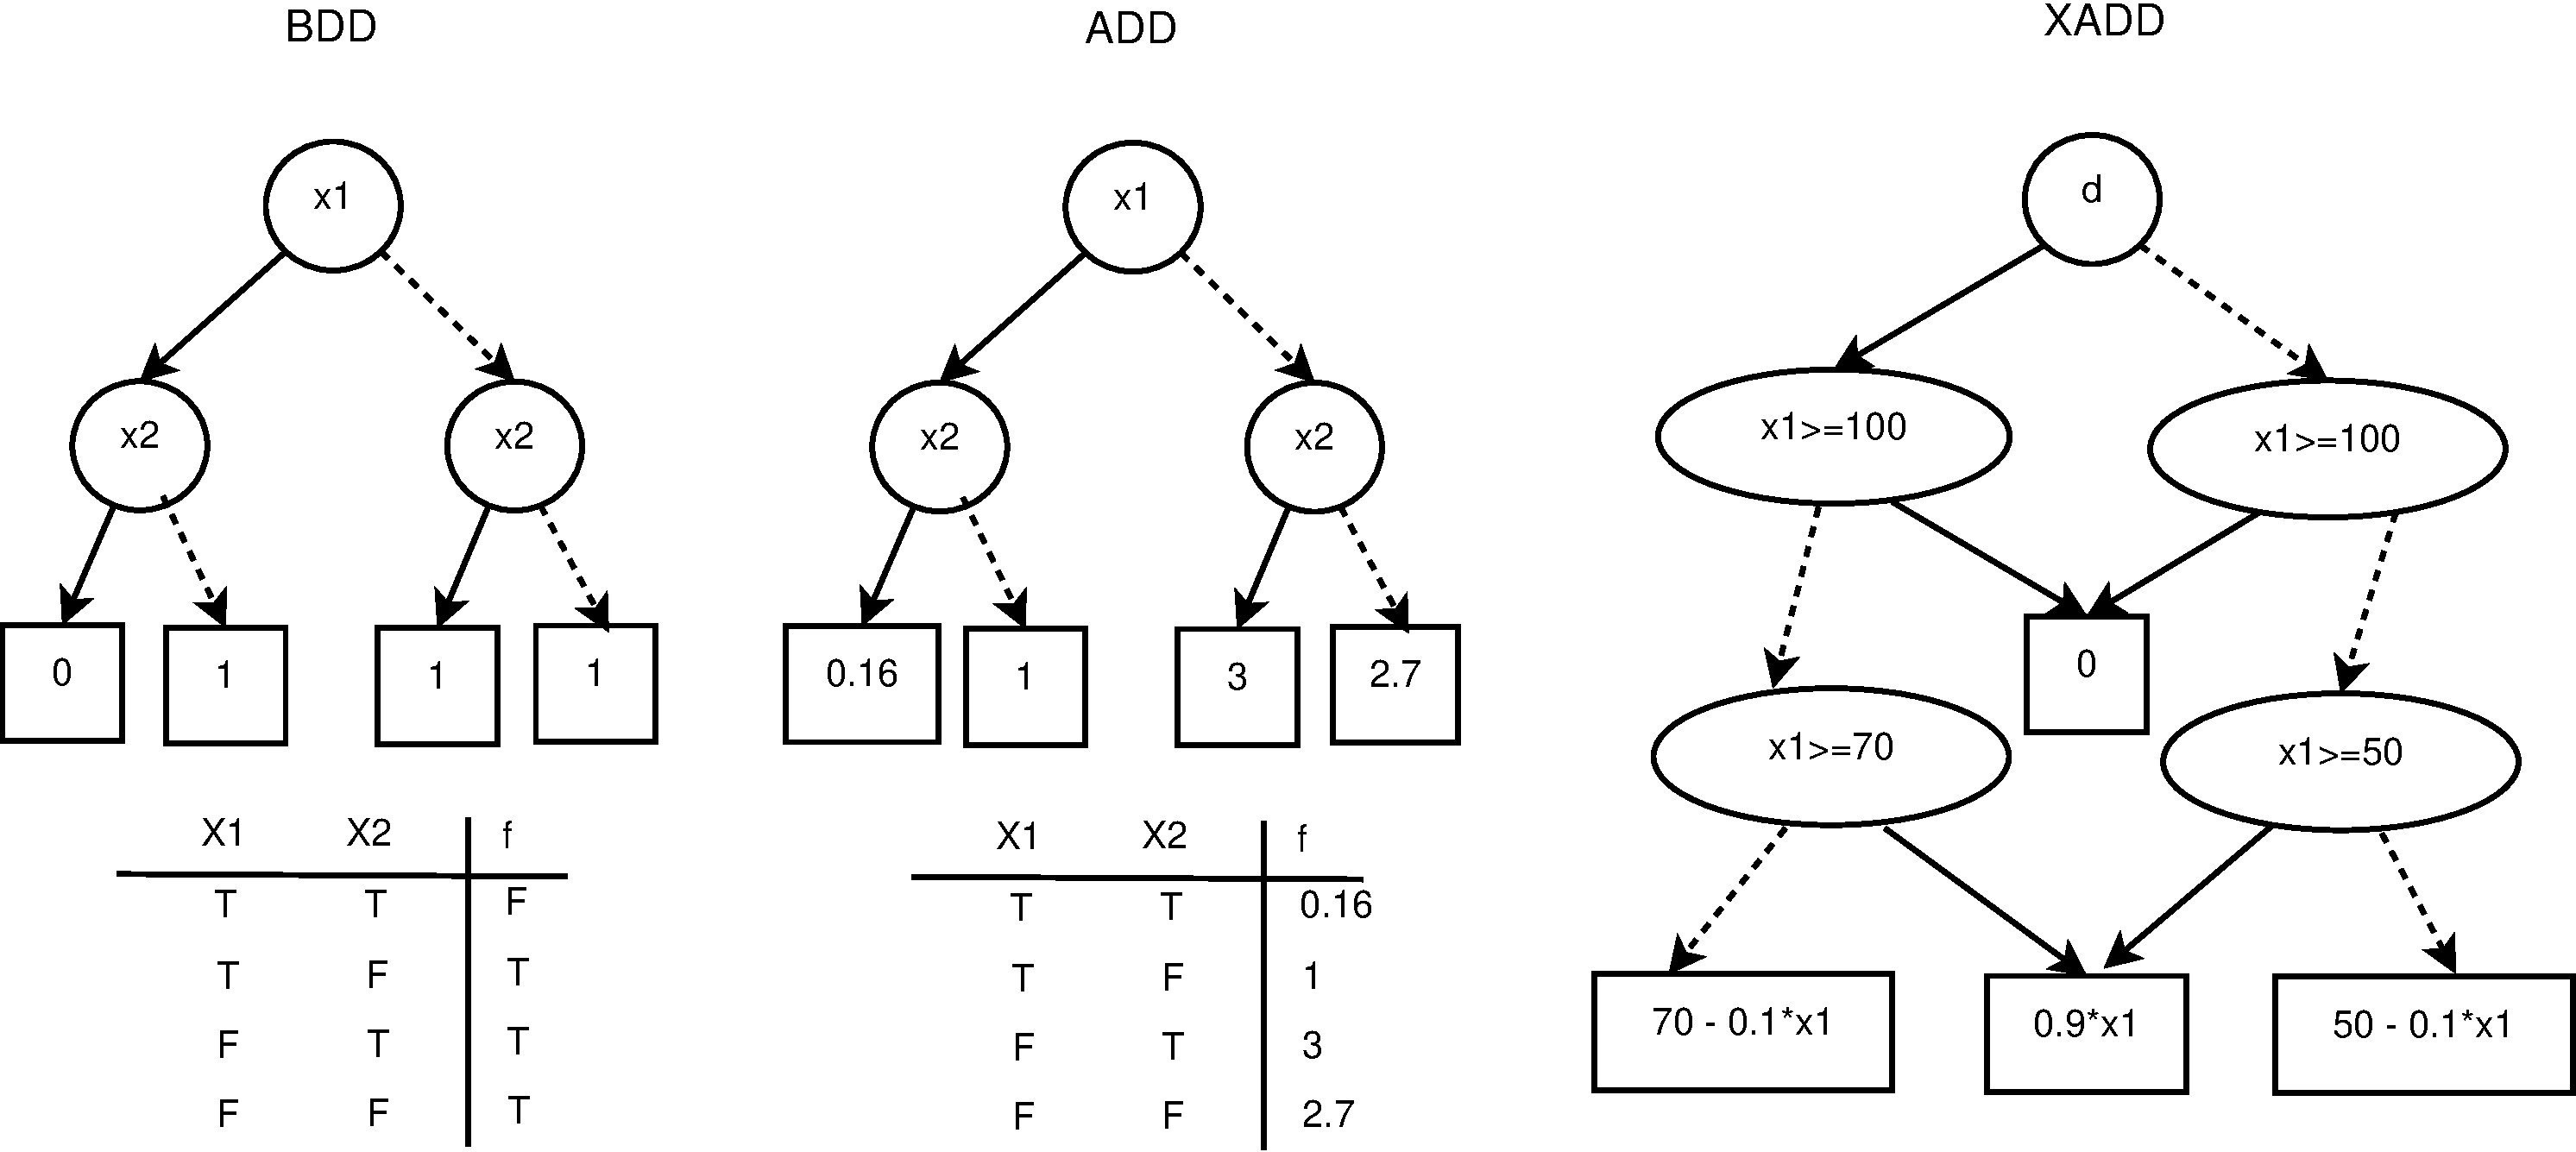
\includegraphics[width=0.8\textwidth]{Figures1/diagrams/bdd_add_xadd.pdf}
\vspace{-2mm}

\caption{\footnotesize Comparison of the three decision diagrams: Binary decision diagrams (BDDs) with boolean leaves and decisions (Left) representing $f(x_1,x_2) = x_1\bar{x_2}+\bar{x_1}$ as shown in the truth table; Algebraic decision diagrams (ADDs) with  boolean decision nodes and real values at the leaves (Middle) represented by the truth table; Extended algebraic decision diagrams (XADDs) with polynomial leaves and decision nodes (Right) demonstrating the reward function (~\ref{rew_inv}) for a 12-item stochastic CAIC problem.}
\label{fig:bdd_add_xadd}
\vspace{-6mm}
\end{figure}
%%%%%%%%%%%%%%%%%%%%%%%%%%%%%%%%%%%%%%%%%%%%%%%%%%%%%%%%%%%%%%%%%%%%%%%%%%
\vspace{-6mm}

Extending BDDs to \emph{algebric decision diagrams} (ADDs) allows a real-value range in the function representation $\lbrace 0,1\rbrace^n \rightarrow \mathbb{R}$. ADDs further provide an efficient representation of \emph{context-specific independent} \cite{bout96} functions (CSI) where node $X$ is independent of nodes $W$ and $V$ given the context $u$ where node ($U=true$). Arithmetic operations can be performed on these functions returning a function value at the leaves; examples include addition
($\oplus$), subtraction ($\ominus$), multiplication ($\otimes$),
division ($\oslash$), $\min(\cdot,\cdot)$ and $\max(\cdot,\cdot)$ \cite{bahar93add}. 

Parameterized ADDs (PADDs) are an extension of ADDs that allow
for a compact representation of functions from $\{0,1\}^{n} \rightarrow
\mathbb{E}$, where $\mathbb{E}$ is the space of expressions
parameterized by $\vec{p}$. Formal definitions of our XADD are similar to that of PADD \cite{spuddip}.

Extended ADDs (XADDs) allow representing continuous variables in a decision diagram in the function representation of $\mathbb{R}^{n+m} \rightarrow \mathbb{R}$ over case statements. Each leaf in an XADD represents a multi-variate arbitrary function from the real-value domain and each decision node can be an equality, dis-equality or inequality on the multi-variate domain which is more expressive than the ADD boolean decisions. The branches are true/false depending on the value of each decision node. This compact representation will not require truth tables like ADDs or BDDs as it is more expressive in allowing infinitely many real values for each decision. 
%note it is NOT about variable assignment! 

We next formally define the XADD operations and algorithms required to support all case operations of SDP as well as pruning algorithms to make this representation even more efficient. 

\subsection{Formal Definition and Operations}
%\vspace*{-0.05in}
% Any other definition except BNF? 
An XADD allows polynomials at the leaves and decisions instead of a single real-value.  According to the set of continuous variables in an XADD $\theta = \lbrace x_1,x_2,...,x_n\rbrace$ and the set of constants $c_i (0 \leq i \leq p)$ each leaf can be canonically defined as:
\begin{equation}
c_0+\sum_{i} c_i \prod_j \theta{ij}
\nonumber
\end{equation}
where $ 1 \leq j \leq n $. Each decision node is an inequality of some polynomial function. Formally an XADD is defined using a BNF grammer: 
\begin{equation}
\nonumber
\begin{array}{lll}
F&::=&  \mathit{Poly}  \hspace{1mm} \vert  \hspace{1mm} \mathrm{if} (F^{var})\ \mathrm{then}\ F_h\ \mathrm{else}\ F_l \\
F^{var}&::=& ( \mathit{Poly} \leq 0)  \hspace{1mm}\vert \hspace{1mm}
 ( \mathit{Poly} \geq 0) \vert \hspace{1mm} B\\
\mathit{Poly}&::=&c_0+\sum_{i} c_i \prod_j \theta_{ij}\\
B&::=& 0|1
\end{array}
\end{equation}
An XADD node $F$ can either be a leaf $\mathit{Poly}$ with a polynomial value or a decision node $F^{var}$ with two branches $F_h$ and $F_l$ which are both of the non-terminal type $F$. The decision node $F^{var}$ associated with a single variable $var$ can be a polynomial inequality or a boolean decision $B = \lbrace b_1,b_2,...,b_m \rbrace$ where each boolean variable $b_k \in \lbrace 0,1 \rbrace$. If $F_h$ is taken the value of the decision node $F^{var}$ is true and if $F_l$ is taken the negation of the decision node $\neg F^{var}$ is set to true.\footnote {Note we assume continuous functions; if a function has the same values on a boundary point (equality), we allow only one of the $\leq, \geq$ at the boundary point. This continuous property allows us to replace $<$ ( $>$ ) with $\leq$($\geq$).} 

The value returned by a function $f$ represented as an XADD ($F$) containing (a subset of) the discrete and continuous variables $\{ b_1,\cdots,b_m, x_1,\cdots, x_n \}$ with variable assignments $\rho \in \lbrace \lbrace\mathit{true}, \mathit{false} \rbrace^m,\mathbb{R}^n \rbrace$ can be defined recursively by:
\begin{equation*}
Val(F,\rho) = \left\{
\begin{array}{lll}
\textrm{if } F=\mathit{Poly} :&\mathit{Poly}\\
\textrm{if } F = \mathit{Poly} \rho(F^{var})=\mathit{true}: & \mathit{Val} (F_h,\rho)\\
\textrm{if } F = \mathit{Poly}  \rho(F^{var})=\mathit{false}: & \mathit{Val} (F_l,\rho)\\
\end{array} \right. 
\end{equation*}

This recursive definition of $Val(F,\rho)$ reflects the structural
evaluation of $F$ by starting at its root node and following
the branch at each decision node corresponding to the decisions taken
in $F^{var}$ --- continuing until a leaf node is reached,
which is then returned as $Val(F,\rho)$. The diagram on the right of Figure ~\ref{fig:bdd_add_xadd} demonstrates the polynomial leaves and the decision node inequalities which branch to true/false depending on the decision value.

%////////////////////////////////proof starting, comment all!
%For BDDs and ADDs proof of canonicity can be defined according to \cite{bryant}. In these two cases for any function $f(x_1,\cdots, x_n)$ and a fixed variable ordering over $x_1,\cdots, x_n$, a reduced BDD or ADD is defined as the minimally sized ordered decision diagram representation of a function $f$. This proves that there is a unique canonical BDD or ADD representation for every function from $\{0,1\}^{n} \rightarrow \{0,1\}$ for BDDs and $\{0,1\}^{n} \rightarrow \mathbb{R}$ for ADDs. 

%To prove such a result for XADDs is not as trivial. In an XADD, leaves and decision nodes are polynomials and we have to prove minimality with respect to this.
%that there exists a unique canonical form for both the leaves and the internal nodes. 
To define the pruning algorithms, we provide some definitions listed below:

\begin{mydef}(\textbf{Function representation}):
A multi-variate function of booleans and real values $ f:\mathbb{B}^m \times \mathbb{R}^n \rightarrow \mathbb{R}$ denoted by $f(\vec{b},\vec{x})$  represents an XADD ($f_{XADD}$) defined on the class of piecewise formulas (case statements).
\end{mydef}

\begin{mydef}(\textbf{Path}):
A path $p$ in $f_{XADD}$ is a sequence of the pair $\rho=(F^{var},\mathit{dec})$ where each node  $F^{var}$ has a unique id and each decision assignment $\mathit{dec} \in \lbrace \mathit{true},\mathit{false}\rbrace$ represents the ( true or false) branch that node $F^{var}$ has followed. Note that the root node $\rho_0=(0,null)$ has a null decision assignment. A path is generally defined as a finite subset (in a sequence) of all possible pairs in $f_{XADD}$.
\begin{equation*}
p_j \subset \lbrace (F_1^{var},\mathit{dec_1}), (F_2^{var},\mathit{dec_2}), \cdots, (F_{n+m}^{var},\mathit{dec_{n+m}}) \rbrace
\end{equation*}
\end{mydef}
where $1 \leq j \leq (n+m)$ is the path number and the last pair on a given path $p_k$ is defined as the \textit{end-node} : $\eta(p_k)$ of that path.

\begin{mydef}(\textbf{Formula}):
The set of all paths for a node $F^{var}$ is defined as all paths $\lbrace p_1 \cdots p_k \rbrace$ ($1 \leq k \leq (n+m)$) such that the end-node of these paths are equal to node $F^{var}$ that is: $\eta(p_k) = F^{var}$. A formula on this node $\psi_{var} $ is defined as this finite set of paths $\psi_{var} = \lbrace p_k | \eta(p_k) = F^{var}, 1 \leq k \leq (n+m) \rbrace$. 
\end{mydef}
%%%%%%%%%%%%%%%%%%%%%%%%%%%%%%%%%%%%%%%%%%%%%%%%%%%%%%%%%%%%%%%%%%%%%%%%%%
\vspace{10mm}
\begin{figure}[t!]
\centering
%\subfigure{
%\hspace{-20mm}
\vspace{-3mm}
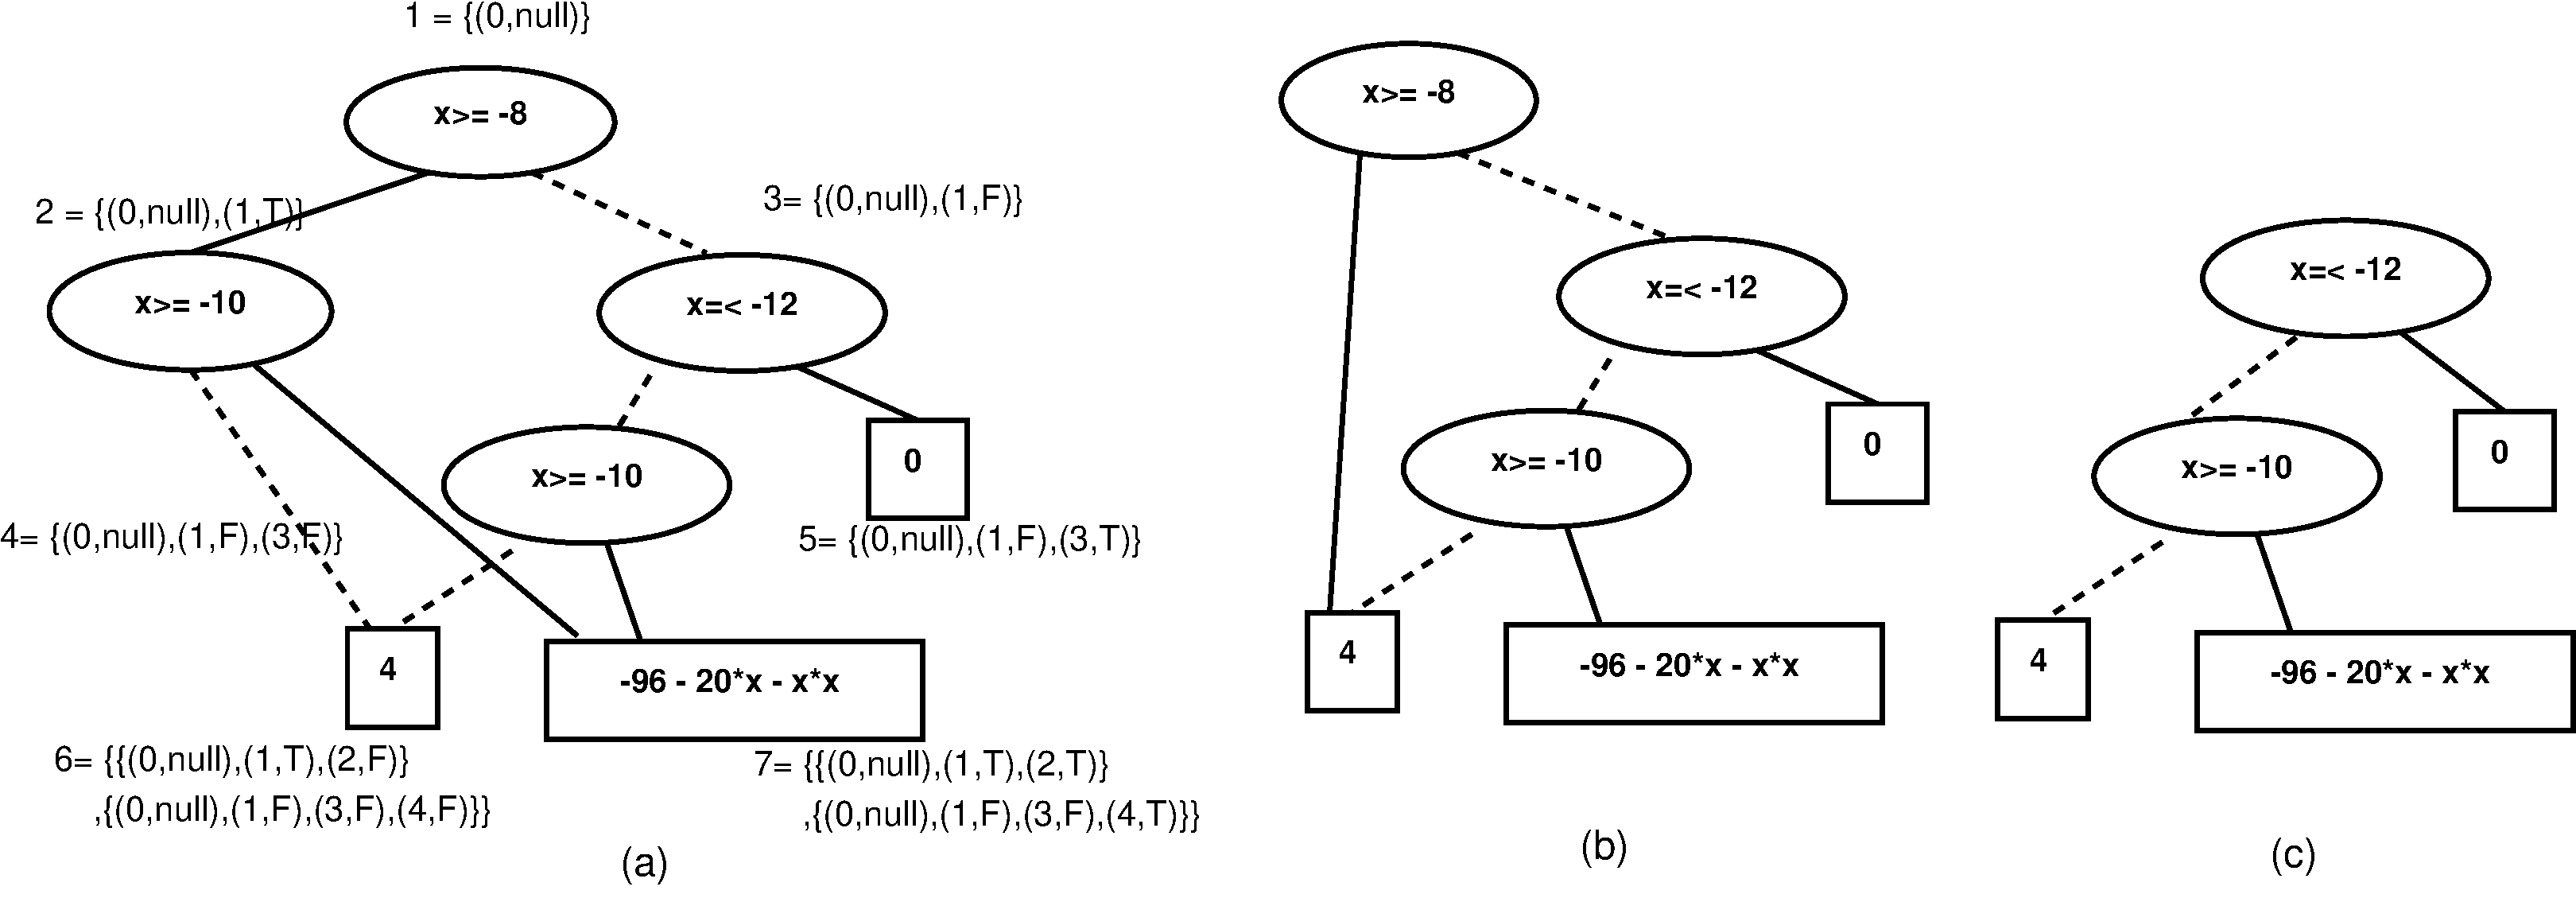
\includegraphics[width=1.0\textwidth]{Figures1/diagrams/path_formula2.pdf}
\vspace{-9mm}
\caption{\footnotesize (a) Path and formula definitions on each node in the XADD. A path is defined as a sequence of the tuple $(F^{var},\mathit{dec})$ and a formula is a set of paths. (b) Pruning inconsistent nodes of (a). (c) Pruning redundant nodes of (b)}
\label{fig:path_formula}
\vspace{-4mm}
\end{figure}
%%%%%%%%%%%%%%%%%%%%%%%%%%%%%%%%%%%%%%%%%%%%%%%%%%%%%%%%%%%%%%%%%%%%%%%%%%
\vspace{-7mm}
To define any node $F^{var}$ in $f_{XADD}$ logically we have the following:
\begin{equation*}
\psi_{var} = \bigvee_{p_j \in p_{var}} (\bigwedge_{\rho_i \in p_j} \rho_i |\eta(p_j) = F^{var})
\hspace{5mm},
\rho_i =
\begin{cases}
  dec_i = \mathit{true}: & F_i^{var} \\ 
dec_i = \mathit{false}: & \neg F_i^{var} \\ 
\end{cases}
\end{equation*} 
Figure ~\ref{fig:path_formula} (a) shows a simple XADD with all paths and formulas determined on each node. %According to the above a sequence of nodes can be expressed using logical-and $\wedge$ on the tuples $p_i \in P$ and each $p_i$ can be defined as a positive or negative literal. As an example node $E$ in Figure ~\ref{fig:path_formula} can be defined as: $E= ( -1 \wedge 3)$. A formula can be represented logically using logical-or $\vee$ of the set of all paths, e.g. $F= (1 \wedge -2)\vee (-1 \wedge -3 \wedge -4)$

\begin{mydef}(\textbf{Node ordering}):
A node $F_i^{var}$ in $f_{XADD}$ is defined before node $F_j^{var}$ if it appears before this node in a path $p_s$ containing both nodes $\rho_i \in p_s, \rho_j \in p_s$ and has an ordering such that $i<j$. $F_j^{var}$ can also be named the child of node $F_i^{var}$. A parent node $F_k^{var}$ is defined for node  $F_i^{var}$ if node  $F_i^{var}$ appears after node $F_k^{var}$ in a path $p_s$ containing both nodes $\rho_i \in p_s, \rho_k \in p_s$ and has an ordering such that $k<i$. In Figure ~\ref{fig:path_formula} (a) node $1$ is the parent of node $3$ and nodes $4,5$ are the children of node $C$.
\end{mydef}

\begin{mydef}(\textbf{Inconsistent node}):
A node $F_i^{var}$ in $f_{XADD}$ is inconsistent if it violates any of the constraints in its parent decision node $F_k^{var}$ in any of the path defined in the formula $\psi_{i}$ over this node. In mathematical terms this is equal to the following: 
 \begin{equation}
\exists p_j \in \psi_i , (\rho_i \in p_j): \exists \rho_k \in p_j, k<i , \phi_i \Rightarrow \phi_k = \textit{true} \longleftrightarrow F_i^{var} = inconsistent. \label{inconsist}
\end{equation} 
where  $\phi_i$ is the logical constraints of node $F_i^{var}$ as defined in case statements. Figure ~\ref{fig:path_formula} (b) prunes (a) of the inconsistent node 2.
\end{mydef}

\begin{mydef}(\textbf{Redundant node}):
A node $F_i^{var}$ in $f_{XADD}$ is redundant if its constraints can be addressed using any of the constraints in its child decision node $F_j^{var}$ in any of the path defined in the formula $\psi_{j}$ over this node. In mathematical terms this is equal to the following: 
 \begin{equation}
\exists p_k \in \psi_j , (\rho_j \in p_k): \exists \rho_i \in p_k, i<j , (\phi_j \Rightarrow \phi_i) \vee (\neg \phi_j \Rightarrow \phi_i) = \textit{true} \longleftrightarrow F_i^{var} = redundant.\label{redundant}
\end{equation} 
Figure ~\ref{fig:path_formula} (c) prunes (b) of the redundant node 1.
\end{mydef}

%In our DCSA-MDP framework we assume polynomial leaves and limit decisions to linear or quadratic inequalities. %In general proving polynomial decisions are canonical is possible using Algebraic geometry given the order of the polynomials, but it is not reasonably computational as there is no bound on the running time. 
%The following corollary proves that there is a canonical form for polynomial functions.

%\begin{corollary} ~\cite{cox}
%Let $k$ be an infinite field, and let $f,g \in k\left[ x_1,\cdots,x_n \right]$ be polynomials over $\left[ x_1,\cdots,x_n \right]$. Then $f=g$ in $k\left[ x_1,\cdots,x_n \right]$ if and only if $f:k^n \rightarrow k$ and $g:k^n \rightarrow k$ are the same function.
%\end{corollary}


%Next we give the formal theorem and proof for a minimal XADD with linear decisions and polynomial leaves.

%\begin{theorem}
%Two functions $f(\vec{b},\vec{x})$  and $g(\vec{b},\vec{x})$  are equal for all $\vec{b},\vec{x}$ if and only if their corresponding XADDs are isomorphic: 
%\begin{equation*}
%\forall \vec{b},\vec{x} : f(\vec{b},\vec{x}) = g(\vec{b},\vec{x}) \hspace{5mm} \Longleftrightarrow \hspace{5mm} f_{XADD}=^i g_{XADD}
%\end{equation*}
%\end{theorem}
%
%\begin{proof}
%The reverse direction of the theorem is easy to prove from the definition of isomorphism. Two isomorphic graphs ( in this case XADDs) have the same number of nodes and and are connected in such a way that their corresponding functions are equal. 
%The other direction is nontrivial and the proof is by induction on the number of nodes of $ f:\mathbb{B}^m \times \mathbb{R}^n \rightarrow \mathbb{R}$. %Each argument $n,m$ is considered as the number of decision levels ($n+m$) for $n$ linear decisions and $m$ boolean decisions.
%
%For ($n = 0,m=0$) there are no linear or boolean decision nodes $D$ and the XADD consists of only a leaf node with a polynomial function. According to Corollary 1.1, two polynomial functions are equal precisely when they give the same function in an infinite space. 
%We can identify when two leaf expressions are identical in practice by the following: \\
%(a) sorting the parameters in each leaf\\
%(b) factoring out (grouping terms with the same ordered set of
%parameters) and summing constants in identical terms\\
%(c) sorting the list of terms according to the lowest variable index
%and number of parameters.  \\
%(d) assigning (+1) to the coefficient of the lowest variable index and dividing the other terms by the coefficient of the lowest variable index. 
%
%We proceed to show the correctness of the theorem for all functions of $n,m$ nodes. We assume two previous cases: (a) For $n,m-1$ if two functions of $ \mathbb{B}^{m-1} \times \mathbb{R}^{n} \rightarrow \mathbb{R}$ are equal then their XADDs are isomorphic. (b) For $n-1,m$ if two functions of $ \mathbb{B}^{m} \times \mathbb{R}^{n-1} \rightarrow \mathbb{R}$ are equal then their XADDs are isomorphic. 
%The additional decision node $d$in both cases is inductively added at the root of two non-equal minimal XADDs $f_{XADD_1},f_{XADD_2}$ and are assigned as the $true$ and $false$ branches of $f_{XADD}$. Note that if $f_{XADD_1}=f_{XADD_2}$ then they are reduced to one graph $f_{XADD_1}$ as defined in the \textit{ReduceXADD} algorithm later and decision $d$ is omitted from the final result. 
%
%For case (a) the new decision node $d$ is a boolean decision node and  $f_{XADD_1} \neq f_{XADD_2}$ then since $d$ is of the order of $m$ it does not occur in any of its left and right subtrees (orthogonal) and there is also no implication between $d$ and $f_{XADD_1}$ or $f_{XADD_2}$. This means that we can't reduce the new XADD any further and this is the unique minimal representation for $f_{XADD}$ and any other function with the same root decision $d$ (since $d$ is boolean, there is a unique canonical representation for it) has to have the same XADD representation. 
%
%If $d$ is a linear inequality as defined by (b), we use Corollary 1.1 to make sure that the function of $d$ is itself canonical. In practice $d$ is a line $\left\langle w_1,\cdots ,w_k \right\rangle \cdot \vec{x} + c = 0$ to make it canonical, we order the coefficients $\left\langle w_1,\cdots ,w_k \right\rangle$ and set the first non-zero coefficient to one ( dividing the other coefficients by this non-zero value).
%
%Next considering $d$ as the root of the two XADDs $f_{XADD_1},f_{XADD_2}$ we need to check for two general cases that can occur because of the relation between the constraint in $d$ and other non-boolean decision nodes: 
%
%\begin{itemize}
%\item  Check whether adding $d$ to $f_{XADD}$ results in any inconsistency in any of $f_{XADD_1}$ or $f_{XADD_2}$. Parts of these canonical XADDs can become inconsistent due to the new constraint added by $d$ to $f_{XADD}$ according to  ~\ref{inconsist}.
%We can remove all inconsistencies using an LP-solver. Starting with the root node, the LP-solver checks for parent-child implications of all the nodes within all paths of $f_{XADD}$. Any inconsistent node is pruned out of  $f_{XADD}$ returning a new XADD where all paths are reachable. Before the next check, we make sure that $f_{XADD_1} \neq f_{XADD_2}$ since otherwise they are collapsed into one minimal XADD of $f_{XADD_1}$ and no further action is required. 
%\begin{equation*}
%(var = f_{XADD}) \equiv (dec_1 \wedge (var=f_{XADD_1}) \vee (dec_2 \wedge (var=f_{XADD_2})): (\neg dec_1 \wedge dec_2 \models \perp)
%\end{equation*}
%
%\item Check whether adding $d$ to $f_{XADD}$ adds redundancy to $f_{XADD_1}$ or $f_{XADD_2}$. Adding $d$ can result in redundant nodes due to the new constraint added by $d$ to $f_{XADD}$ according to ~\ref{redundant}. We can remove all redundancies using a SAT-solver. Satisfiability (SAT) is the problem of determining if the variables of a given Boolean formula can be assigned in such a way as to make the formula evaluate to TRUE. A SAT-solver requires a knowledge base of all true formulas to check the satisfiability of a new formula. 
%
%Starting at the root node, all possible child-parent implications are added  to the knowledge-base of the SAT-solver. At the end-node of each path $\eta(p_i)$, the SAT-solver checks for all redundant nodes for all paths of $f_{XADD}$. If the formula $\psi$ at any decision node $n$ is equivalent to taking the $true$ or $false$ branch of $n$ with respect to the KB, then the SAT-solver identifies this node as a redundant node and it is pruned out of $f_{XADD}$: 
%\begin{equation*}
%(\psi_n \Longleftrightarrow^{KB} (\psi_{n_\mathit{True}}) \vee (\psi_{n_\mathit{False}})) \Longrightarrow \mathit{Prune} \hspace{2mm} n
%\end{equation*}
%
%\end{itemize}
%Thus if we add the new decision in any order in the canonical XADD of $n$, given that any inconsistency or redundancy is removed in polynomial decisions and also the format of the decision is also canonical, the new XADD of order $n+1$ is also canonical. 
%\end{proof}

For any function from $\mathbb{R}^{n+m} \rightarrow \mathbb{R}$, we next
describe how a reduced XADD can be constructed from an arbitrary ordered decision diagram.
All algorithms that we will define in the following sections rely on the helper function \emph{getNode} in Algorithm \ref{algGetNode} , which returns a more compact representation of a single internal decision node. 

The algorithm \emph{ReduceXADD} allows the construction of a compact XADD representation from an arbitrary ordered decision diagram with polynomial leaves and polynomial inequalities as the decision nodes. Algorithm~\ref{algReduceXADD} is defined according to the following definition: 
%%%%%%%%%%%%%%%%%%%%%%%%%%%%%%%%%%%%%%%%%%%%%%%%%%%%%%%%%%%%%%%%%
\incmargin{1em}
\linesnumbered
\begin{algorithm}[t!]
\SetKwFunction{getNode}{{\sc GetNode}}
\SetKwFunction{reduce}{{\sc ReduceXADD}}
\SetKwInOut{Input}{input}
\SetKwInOut{Output}{output}

\Input{$F$ (root node id for an arbitrary ordered decision diagram)}
\Output{$F_r$ (root node id for reduced XADD)}
\BlankLine
\Begin{
   //if terminal node, return canonical terminal node\\
   \If{F is terminal node}
   {
   \Return{canonical terminal node for polynomial of $F$}\;
   }
   //use recursion to reduce sub diagrams\\
   \If{$F \rightarrow F_r$ is not in ReduceCache}
   {
    $F_h$ = \reduce{$F_h$}\;
    $F_l$ = \reduce{$F_l$}\;
    //get a canonical internal node id\\
    $F_r$ = \getNode{$F^\mathit{var}$, $F_h$, $F_l$}\;
    insert $F \rightarrow F_r$ in ReduceCache\;
   } 
   \Return{$F_r$}\;
}
\caption{{\sc ReduceXADD}(F)  \label{algReduceXADD}}
\end{algorithm}
\decmargin{1em}
%%%%%%%%%%%%%%%%%%%%%%%%%%%%%%%%%%%%%%%%%%%%%%%%%%%%%%%%%%%%%%%%%
%%%%%%%%%%%%%%%%%%%%%%%%%%%%%%%%%%%%%%%%%%%%%%%%%%%%%%%%%%%%%%%%%
\begin{algorithm}[t!]
\SetKwInOut{Input}{input}
\SetKwInOut{Output}{output}

\Input{$\langle \mathit{var}, F_h, F_l \rangle $ (variable and true and false branches node ids for internal node)}
\Output{$F_r$ (canonical internal node id)}
\BlankLine
\Begin{
   //redundant branches\\
   \If{$F_l = F_h$}
   {
      \Return{$F_l$}\;
   }
   //check if the node exists previously\\
   \If{$\langle \mathit{var}, F_h, F_l \rangle \rightarrow \mathit{id}$ is not
   in NodeCache}
   {id\ = new unallocated id\;  
    insert $\langle \mathit{var}, F_h, F_l \rangle \rightarrow \mathit{id}$ in NodeCache\;
   }
   \Return{id}\;
}
\caption{{\sc GetNode}($\langle \mathit{var}, F_h, F_l
\rangle $)  \label{algGetNode}}
\end{algorithm}
%%%%%%%%%%%%%%%%%%%%%%%%%%%%%%%%%%%%%%%%%%%%%%%%%%%%%%%%%%%%%%%%%

\textbf{Definition:} A function graph G is reduced if it contains no vertex $v$ with $low(v)=high(v)$, nor does it contains distinct vertices $v$ and $v′$ such that the subgraphs rooted by $v$ and $v′$ are isomorphic.

This algorithm recursively constructs a reduced XADD from the bottom up. Internal nodes are represented as $\langle F^{\mathit{var}}, F_h, F_l \rangle$, where $F^{\mathit{var}}$ is the variable name, and $F_h$ and $F_l$ are the true and false branch node ids, respectively. Reduced nodes are stored in the \emph{ReduceCache} table.
Using the function \emph{GetNode} (Algorithm\ref{algGetNode}) any redundant decision tests are removed. This function stores a unique id for each node in the \emph{NodeCache} table. 

\emph{ReduceCache} ensures that each node is visited once and a unique reduced node is generated in the final diagram. Thus \emph{ReduceXADD} has linear running time and space according to the size of the input graph. 

%%%%%%%%%%%%%%%%%%%%%%%%%%%%%%%%%%%%%%%%%%%%%%%%%%%%%%%%%%%%%%%%%%%%%%%%%%%
\vspace{10mm}
\begin{figure}[t!]
\centering
%\subfigure{
%\hspace{-20mm}
\vspace{-3mm}
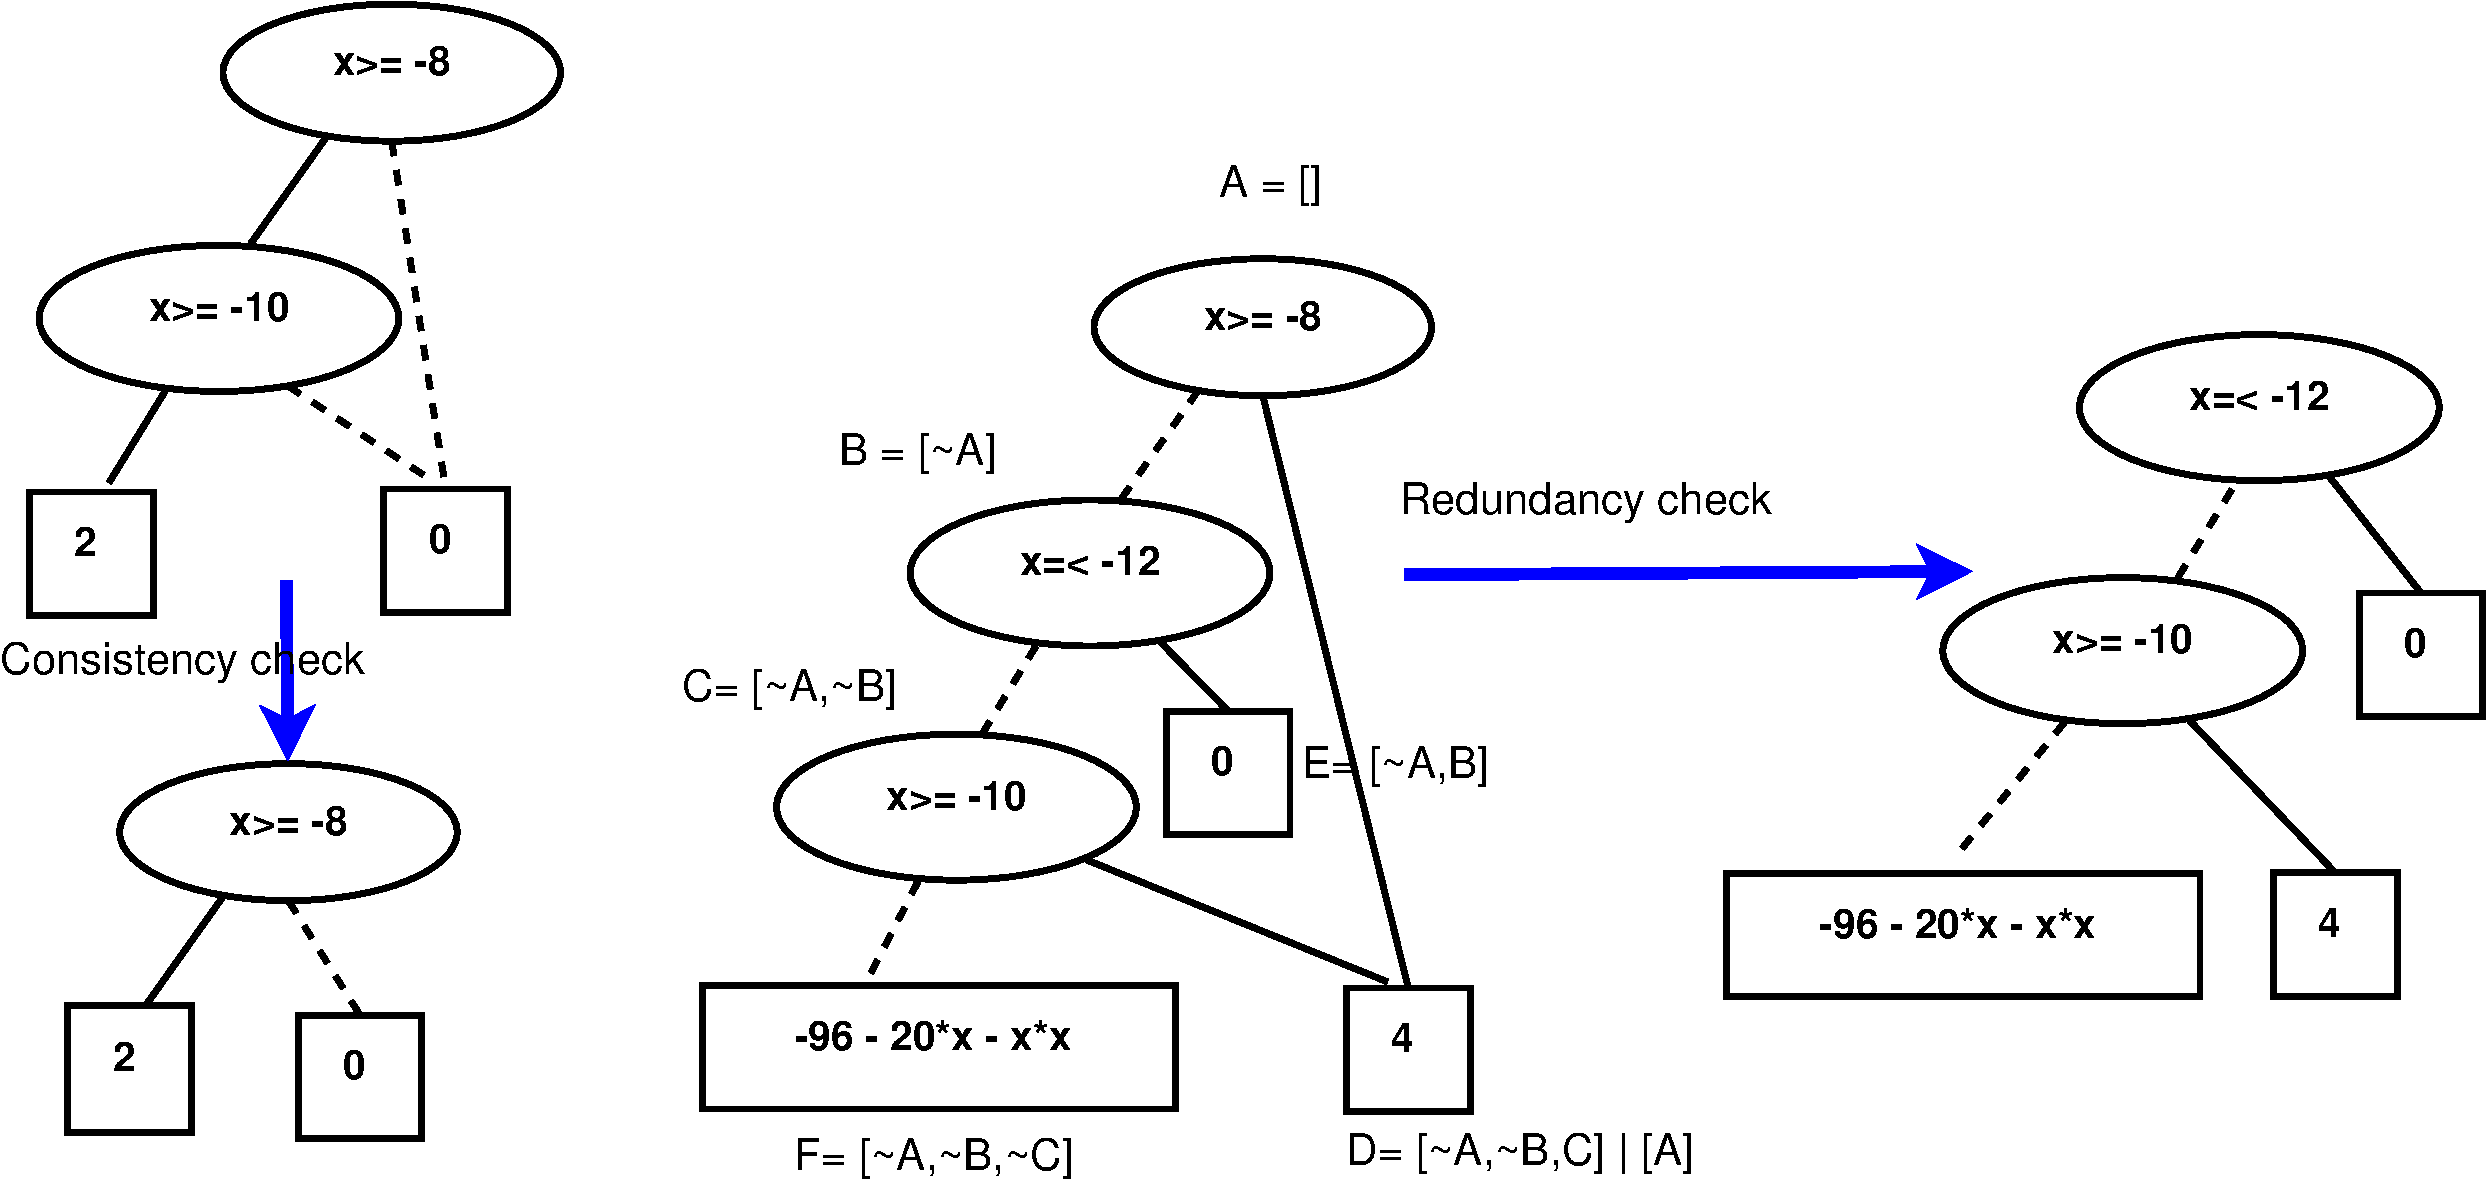
\includegraphics[width=0.8\textwidth]{Figures1/diagrams/redundancy.pdf}
\vspace{-2mm}

\caption{\footnotesize Using pruning algorithms for inconsistency and redundancy. Top-left figure is reduced to the bottom-left figure using the LP-Solver which recognizes the parent-child relation. The middle figure is reduced to the right-most figure using the SAT-Solver. The paths of each node in the middle graph are demonstrated. These paths along with the child-parent implications in the KB can reduce the redundant node A.}
\label{fig:canonical}
\vspace{-6mm}
\end{figure}
%%%%%%%%%%%%%%%%%%%%%%%%%%%%%%%%%%%%%%%%%%%%%%%%%%%%%%%%%%%%%%%%%%%%%%%%%%%
%\vspace{-7mm}
We next present two successive algorithms, Algorithm~\ref{algPrune} for removing inconsistent nodes and Algorithm~\ref{algRedundant} for removing redundant nodes. 
Given any XADD with potential inconsistent nodes, the output of \emph{algPrune} (Algorithm~\ref{algPrune}) is a reduced XADD with canonical leaves, linear decisions and no inconsistent nodes. 
In lines 7 and 11 we test the current decision node with all previous decisions for implications in \emph{TestImplied}. 
This process is performed using the definition of constraints for the LP-solver. Once a node is returned inconsistent (returns true or false from \emph{TestImplied}) the high or low branch is returned without referring to the current node in the final XADD. 

While any (parent(A) $\Rightarrow$ child(B)) relation is returned for consistency checking, at the same time this function stores other implications in the a related cache ($\mathit{hmImplications}$). Since $A \Rightarrow B$ is already tested, we cache the following child to parent implications: (i) $B \Rightarrow A$ (2)$\neg B \Rightarrow A$ ($\neg B \Rightarrow \neg A$ is already defined by $A \Rightarrow B$).We add these to the knowledge-base (KB) of the SAT-Solver before performing the next recursive algorithm. 
Lines 14--15 define the decision labels and their values ($\mathit{true,false}$) for the current node and add them to the set of labels and decisions which are input to the algorithm. The final result is returned from the \emph{GetNode} algorithm. 
%%%%%%%%%%%%%%%%%%%%%%%%%%%%%%%%%%%%%%%%%%%%%%%%%%%%%%%%%%%%%%%%%
\incmargin{1em}
\linesnumbered
\begin{algorithm}[t!]
\SetKwFunction{getNode}{{\sc GetNode}}
\SetKwFunction{testImplied}{{\sc TestImplied}}
\SetKwFunction{prune}{{\sc PruneInconsistent}}
\SetKwInOut{Input}{input}
\SetKwInOut{Output}{output}

\Input{$F$ (root node id for an inconsistent XADD, Decision label, Decision value)}
\Output{$F_r$ (root node id for a consistent XADD)}
\BlankLine
\Begin{
   //if terminal node, return the value\\
   \If{F is terminal node}
   {
    \Return{canonical terminal node for polynomial of $F$}\;
   }
   //else if internal node, find all implications consider any parent in XADD\\
   
    	//if (parent$\Rightarrow$ child) remove child\\
    	 \If{\testImplied{$\mathit{decLabel}$,$\mathit{decision}$,$F^\mathit{var}$}}
    			{$F_r$ = \prune{$F_h$,$\mathit{decLabel}$,$\mathit{decision}$}\;}
    	//if (parent$\Rightarrow$ $\neg$child) remove child\\
    	 \If{!\testImplied{$\mathit{decLabel}$,$\mathit{decision}$,$- F^\mathit{var}$}}
    			{$F_r$ = \prune{$F_l$,$\mathit{decLabel}$,$\mathit{decision}$}\;}
  //if result of LP-solver is null\\
   \Else
   {	
     insert $F^{var} \rightarrow \mathit{decLabel}$\;
     insert $\mathit{false} \rightarrow \mathit{decision}$\;
    $F_r^l=$  \prune{$F_l$,$\mathit{decLabel}$,$\mathit{decision}$}\;
     insert $\mathit{true} \rightarrow \mathit{decision}$\;
    $F_r^=$  \prune{$F_h$,$\mathit{decLabel}$,$\mathit{decision}$}\;	 
     insert $\mathit{null} \rightarrow \mathit{decision}$\;
     delete $F^{var} \rightarrow \mathit{decLabel}$\;

    $F_r=$ \getNode{$var,F_r^h,F_r^l$}\;
	}
   \Return{$F_r$}\;
}
\caption{{\sc PruneInconsistent}(F,$\mathit{decLabel}, \mathit{decision}$)  \label{algPrune}}
\end{algorithm}
\decmargin{1em}
%%%%%%%%%%%%%%%%%%%%%%%%%%%%%%%%%%%%%%%%%%%%%%%%%%%%%%%%%%%%%%%%%
%%%%%%%%%%%%%%%%%%%%%%%%%%%%%%%%%%%%%%%%%%%%%%%%%%%%%%%%%%%%%%%%%
\incmargin{1em}
\linesnumbered
\begin{algorithm}[t!]
\SetKwFunction{getNode}{{\sc GetNode}}
\SetKwFunction{sat}{{\sc Sat-Test}}
\SetKwFunction{prune}{{\sc PruneRedundancy}}
\SetKwInOut{Input}{input}
\SetKwInOut{Output}{output}
\Input{$X$ (root node id for a consistent XADD), $KB$ (child-parent implications), $F$ (formulas for each node)}
\Output{$X_r$ (root node id for a consistent and redundant XADD)}
\BlankLine
\Begin{
	//current node is X, keep its path\\
	$\mathit{Path}:=F(X)$\;
   \If{F is terminal node}
   {
    \Return{canonical terminal node for polynomial of $F$}\;
   }
   //else if internal node, add paths to low and high branch\\
   \ForEach{$\mathit{path} \in$  $\mathit{Path}$ }
   {
    	//add high and low branch of internal node to current path\\
    	insert $X_r \rightarrow  \mathit{path};$
    	add $\mathit{path} \rightarrow F$	\; 
    	insert $X_l \rightarrow  \mathit{path};$
    	add $\mathit{path} \rightarrow F$	\;
    	
    }	
    $X_l=$  \prune{$X_l,KB,F$}\;
    $X_h^=$  \prune{$X_h,KB,F$}\;	 
   
   //reached the lowest decision node, perform satisfiability test\\
    \If{\sat{$X$,$F(X_l),KB,T$}}
    	{ \Return{$X_h$}\;}
    \If{\sat{$X$,$F(X_h),KB,F$}}
    	{ \Return{$X_l$}\;}
   
    $X_r=$ \getNode{$var,X_h,X_l$}\;
	
   \Return{$X_r$}\;
}
\caption{{\sc PruneRedundancy}(X,KB,F)  \label{algRedundant}}
\end{algorithm}
\decmargin{1em}
%%%%%%%%%%%%%%%%%%%%%%%%%%%%%%%%%%%%%%%%%%%%%%%%%%%%%%%%%%%%%%%%%
%\vspace{-3mm}
As an example consider the two cases on the left side of the Figure ~\ref{fig:canonical}. In the upper diagram,  $x \geq -8  \Rightarrow x \geq -10 $ is reduced to $x\geq-8$ since it covers all the state space in the lower diagram.   

Next we propose an equivalence testing approach for redundancy pruning using a SAT-solver. Consider the middle example in Figure  ~\ref{fig:canonical} where the child node(C) implies the parent node(A). We define the recursive algorithm required to prune all child-parent implications from an XADD using this example. We introduce Algorithm \ref{algRedundant} to remove redundant nodes. 
The input to this algorithm is an XADD where each node $F^{var}$ is marked with its formula $\psi_{var}$ (set of paths) as in the middle diagram of Figure  ~\ref{fig:canonical}. 

The recursive property of the algorithm now traverses backwards from the leaf nodes up to the root node. Every time a decision node is reached (A), the true and false branches of that node are put to a satisfiability test (\emph{Sat-Test}) to see if that branch can be eliminated from the tree due to some child-parent implication. A query is built to test the KB according to the current decision node. At node A, we test to see if the false or true branch can be removed. Considering the true branch we look for the equivalence of reaching leaf D (value 4) with the whole tree or only considering the false branch of A ( which is equal to pruning out the true branch). We test the formulas $\psi_{A=F/T} \Longleftrightarrow \psi$ where each F is the disjunct of all paths leading to this node (D). The KB here contains the child-parent implication of $C \Rightarrow \neg A$ For this example this is equal to the following satisfiability test: 
\begin{equation*}
(B \Rightarrow A) \models ((A \vee (\neg A \wedge \neg B \wedge C))\Longleftrightarrow(\mathit{false} \vee (\mathit{true} \wedge \neg B \wedge C)))
\end{equation*}

We use a SAT-solver (minisat) to entail this sentence and since the result is true, we can prune the true branch returning node B represented in the right-hand diagram of  Figure ~\ref{fig:canonical}. A similar approach is performed for the high branch in lines 16--17. The returned value is the true or false branch if the parent node can be pruned else a new node is built using line 19 of Algorithm \ref{algGetNode}. 

In principle exact SDP solutions can be obtained for arbitrary symbolic functions, we  restrict XADDs to use polynomial functions only. %This allow unique and canonical form for all functions and equations in the decision nodes and leaves, which further minimizes redundancy in an XADD.
Having proved the main properties of an XADD, next we present the operations and algorithms required for SDP for XADDs.

\subsection{XADD algorithms and operations}

In this section we review the symbolic operations required to perform SVI using the XADD structure. This is mainly categorized into unary and binary operations.   

%%%%%%%%%%%%%%%%%%%%%%%%%%%%%%%%%%%%%%%%%%%%%%%%%%%%%%%%%%%%%%%%%
%\incmargin{1em}
%\linesnumbered
\begin{algorithm}[t!]
\SetKwFunction{getCanonicalNode}{{\sc GetCanonicalNode}}
\SetKwFunction{reduce}{{\sc Reorder}}
\SetKwInOut{Input}{input}
\SetKwInOut{Output}{output}

\Input{$F$ (root node for possibly unordered XADD)}
\Output{$F_r$ (root node for an ordered XADD)}
\BlankLine
\Begin{
   //if terminal node, return canonical terminal node\\
   \If{F is terminal node}
   {
   \Return{canonical terminal node for polynomial of $F$}\;
   }
   //else nodes have a $\mathit{true}$ \& $\mathit{false}$ branch and $\mathit{var}$ id\\
   \If{$F \rightarrow F_r$ is not in Cache}
   {
    $F_{\mathit{true}}$ = \reduce{$F_{\mathit{true}}$} $\otimes \; \mathbb{I}[F_\mathit{var}]$ \;
    $F_{\mathit{false}}$ = \reduce{$F_{\mathit{false}}$} $\otimes \; \mathbb{I}[\neg F_\mathit{var}]$\;
    $F_r = F_{\mathit{true}} \oplus F_{\mathit{false}}$\;
    insert $F \rightarrow F_r$ in Cache\;
   } 
   \Return{$F_r$}\;
}
\caption{{\sc Reorder}(F)  \label{alg:reorder}}
\end{algorithm}
%\decmargin{1em}
%%%%%%%%%%%%%%%%%%%%%%%%%%%%%%%%%%%%%%%%%%%%%%%%%%%%%%%%%%%%%%%%%
\subsubsection{Unary XADD Operations}
According to the previous section on SDP unary operations, scalar multipication $c.f$ and negation $- f$ on a function results in a function which can simply be represented as an XADD. Apart from this restriction, substitution and marginalization of the $\delta$ function are also unary operations that can be applied to XADDs are explained below.  

Restriction of a variable $x_i$ in an XADD ($F$) to some formula $\phi$ is performed by appending $\phi$ to each of the decision nodes while leaves are not affected. %The true of false branches according to $\phi_i \wedge \phi$ instead of $\phi_i$.
For a binary variable restriction to a single variable $x_i$ is equal to taking the true or false branch according to that variable 
($F|_{x_i=true}$) or ($F|_{x_i=false}$). 
This operation can also be used to $\texttt{marginalize}$ or $\texttt{sum\_out}$ boolean variables in a DCSA-MDP. 
$\sum_{x_i \in X_i}$ eliminates a variable $x_i$ from an XADD and computed as the sum of the \emph{true} and \emph{false} restricted functions ($F|_{x_i=true} \oplus \ F|_{x_i=false}$). We omit the restriction and marginalization algorithms for XADDs since they are identical to the same operations for ADDs. 

Substitution for a given function $f$ is performed by applying $\sigma$ the set of variables and their substitutions to each inequality operand such that $\phi_i\sigma: f_i\sigma$. The substitution operand effects both leaves and decision nodes and changes them according to the variable substitute. 

Decisions become unordered when substituted and also when we perform maximum or minimum explained in the next section. A reorder algorithm has to be applied to the result of the substitution operand. As Algorithm ~\ref{alg:reorder} shows, we recursively apply the binary ADD operations of $\otimes$ and $\oplus$ to decision nodes to reorder the XADD after a substitution. 

As for the integration of the $\delta$-function on variable $x$ we require computing $\int_{x} \delta [ x - g(\vec{x})]fdx$. This triggers the substitution $f \lbrace x/ g(\vec{x})\rbrace$ on $f$ as defined above.  

For the continuous maximization $max_y$ each XADD path from root to leaf node is considered a single case partition with conjunctive constraints, and maximization is performed at each leaf subject to these constraints and all path maximums are then accumulated using the \textit{casemax} operation for the final result. Note that in general continuous maximization is a multi-variate operation but according to the previous section, it can be decomposed into multiple univariate operations. 

%%%%%%%%%%%%%%%%%%%%%%%%%%%%%%%%%%%%%%%%%%%%%%%%%%%%%%%%%%%%%%%%%%%%%%%%%%
\vspace{10mm}
\begin{figure}[t!]
%\centering
%\subfigure{
\hspace{-20mm}
\vspace{-15mm}
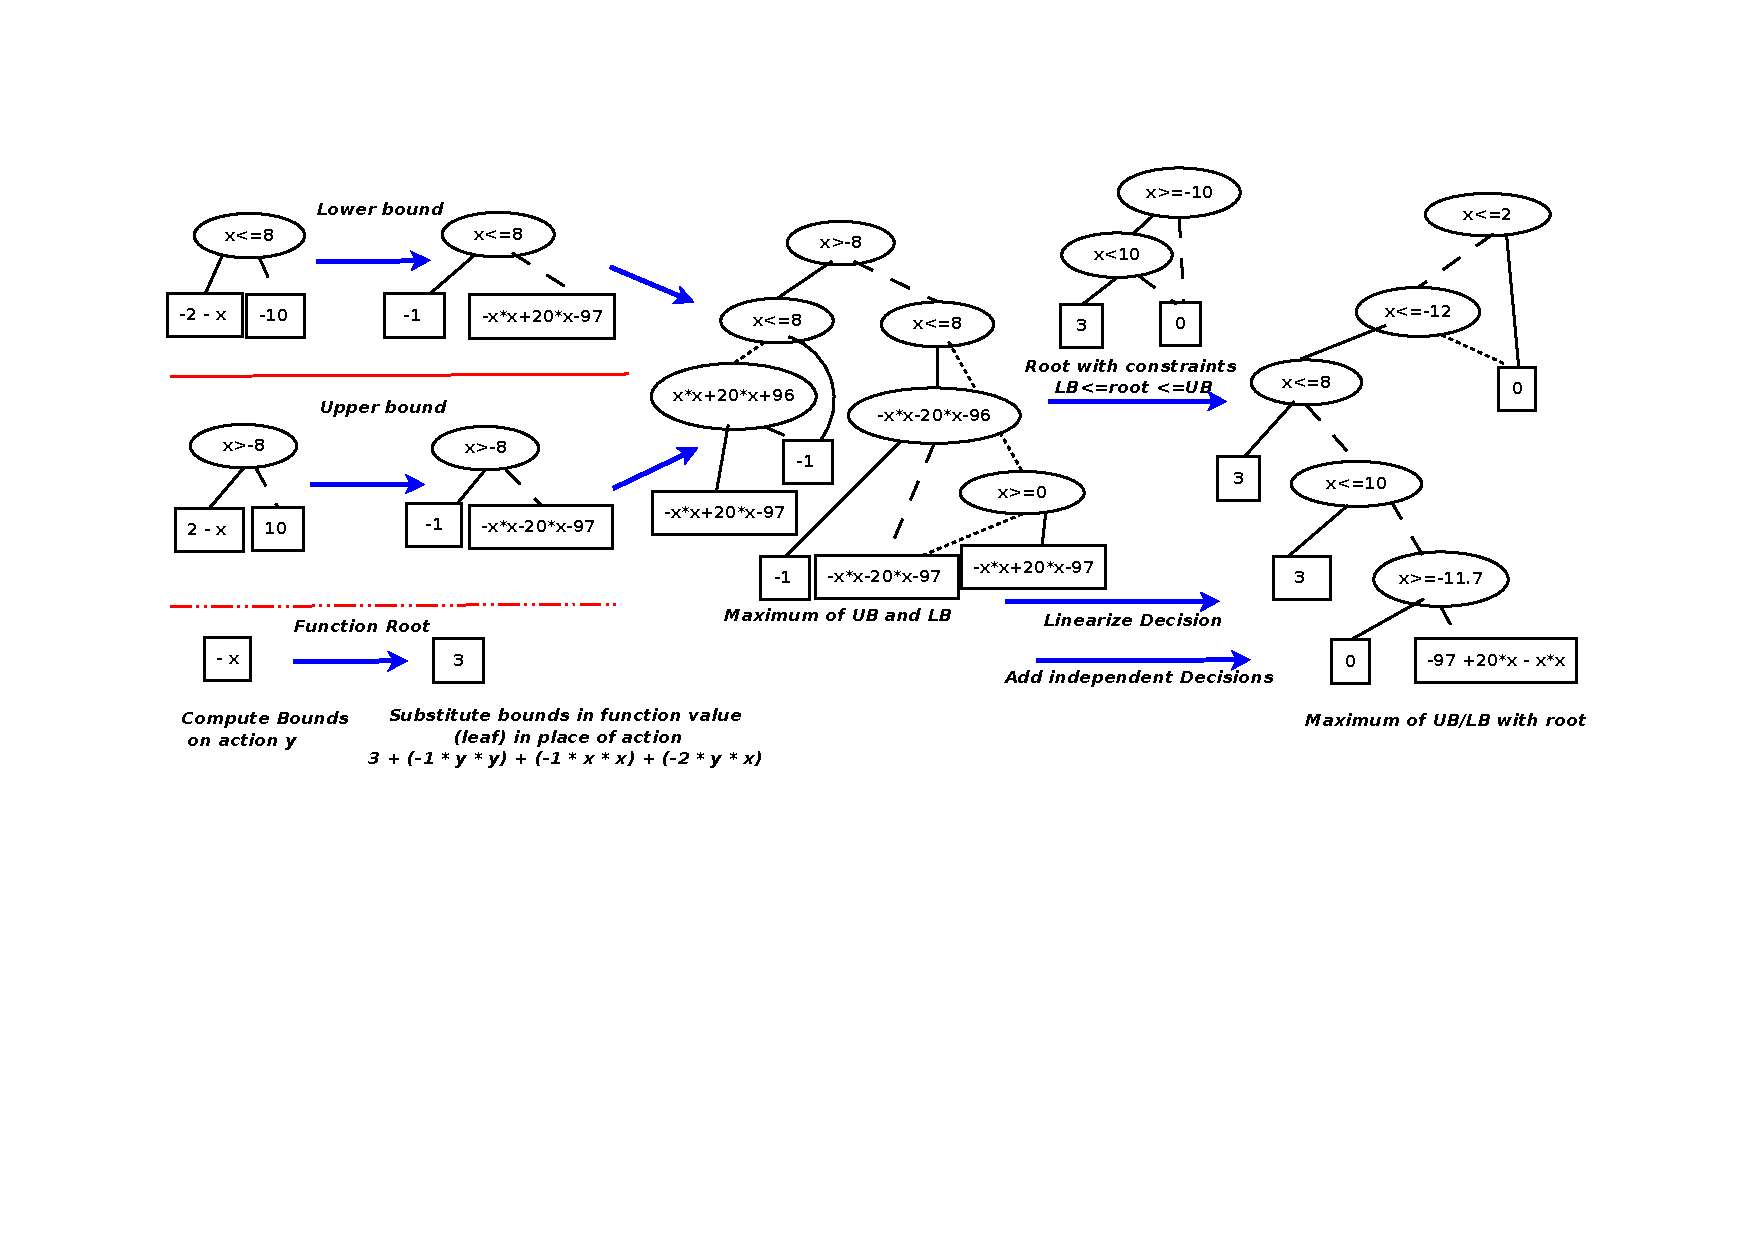
\includegraphics[width=1.27\textwidth]{Figures1/diagrams/maximum_cont_action2.pdf}
\vspace{-40mm}

\caption{\footnotesize Representing one step of Continuous Maximization algorithm using XADDs. The upper and lower bounds of action $a$ and the root is represented by XADDs and substituted inside the leaf node. The maximum of the upper and lower bound is then represented. The final result takes the maximum of this and the root considering the constraints and independent decisions and also linearizing the decision nodes.}
\label{fig:xadd_max}
\vspace{-8mm}
\end{figure}
%%%%%%%%%%%%%%%%%%%%%%%%%%%%%%%%%%%%%%%%%%%%%%%%%%%%%%%%%%%%%%%%%%%%%%%%%%
\vspace{-6mm}

A univariate continuous maximization algorithm has been presented in the previous section. 
Starting at the root node, if the current node is a decision node, the algorithm is recursively calls on the low and high branches of this node. If the current node is a leaf node, it processes the leaf according to \emph{Continuous Maximization}. The input to this algorithm is the leaf node and the decisions leading to this leaf node i.e., partitioning of the state-action space. The algorithm finds the maximum value according to XADDs used for the upper and lower bounds as well as the function roots. The maximum XADD resulting from these three XADDs along with applying the independent constraints define the final result. A single step of this algorithm is presented in Figure ~\ref{fig:xadd_max}. The input to this step is the leaf node obtained after the regression step of Algorithm \ref{alg:regress}. Also as an input are the decisions leading to this leaf (taking the high or low branches).  The XADD representation is used to represent all intermediate results as well as the final result. 

In order to solve the problem of non-linear problem domains we require a continuous maximization of the continuous action variable $y$ over a non-linear function. This maximization is performed symbolically as explained in section (2.4) by incooperating the non-linear terms at the nodes inside decision nodes. This does not effect our symbolic solution but in order to prune the resulting value function  using the LP-solver explained next, we require linear decisions. 

The linearize algorithm (Algorithm \ref{algLinearize}) presented here is of a recursive nature similar to other XADD algorithms. For each node in the XADD starting at the root node, the algorithm linearizes the decision node and returns the two ( or more) decision nodes replacing that single non-linear node. It then  iterates on the low and high branches of the decision node until it returns all the leaves. The linearization process finds the roots of the non-linear function \emph{GetRoots} in decision nodes it visits and replaces the non-linear decision of linearized decisions which are the roots of the function in the non-linear decision node. 			
			%%%%%%%%%%%%%%%%%%%%%%%%%%%%%%%%%%%%%%%%%%%%%%%%%%%%%%%%%%%%%%%%%
\incmargin{1em}
\linesnumbered
\begin{algorithm}[t!]
\SetKwFunction{getRoots}{{\sc GetRoots}}
\SetKwFunction{reduce}{{\sc ReduceLinearize}}
\SetKwInOut{Input}{input}
\SetKwInOut{Output}{output}

\Input{$F$ (root node id for an arbitrary ordered decision diagram)}
\Output{$F_r$ (root node id for linearized XADD)}
\BlankLine
\Begin{
   //if terminal node, return canonical terminal node\\
   \If{F is terminal node}
   {
   \Return{canonical terminal node for polynomial of $F$}\;
   }
    \If{$F \rightarrow F_r$ is not in ReduceCache}
   {
   //use recursion to reduce sub diagrams\\
    $F_h$ = \reduce{$F_h$}\;
    $F_l$ = \reduce{$F_l$}\;
    //get a linearized internal node id\\
    $F_r$ = \getRoots{$F^\mathit{var}$, $F_h$, $F_l$}\;
    insert $F \rightarrow F_r$ in ReduceCache\;
   } 
   \Return{$F_r$}\;
}
\caption{{\sc ReduceLinearize}(F)  \label{algLinearize}}
\end{algorithm}
\decmargin{1em}
%%%%%%%%%%%%%%%%%%%%%%%%%%%%%%%%%%%%%%%%%%%%%%%%%%%%%%%%%%%%%%%%%	
%%%%%%%%%%%%%%%%%%%%%%%%%%%%%%%%%%%%%%%%%%%%%%%%%%%%%%%%%%%%%%%%%%%%%%%%%%
%\vspace{10mm}
%\begin{figure}[t!]
%%\centering
%%\subfigure{
%\hspace{-20mm}
%\vspace{-15mm}
%\includegraphics[width=1.27\textwidth]{Figures1/diagrams/reorder.pdf}
%\vspace{-40mm}
%
%\caption{\footnotesize reordering substitute and max.}
%\label{fig:reorder}
%\vspace{-8mm}
%\end{figure}
%%%%%%%%%%%%%%%%%%%%%%%%%%%%%%%%%%%%%%%%%%%%%%%%%%%%%%%%%%%%%%%%%%%%%%%%%%

\subsubsection{Binary XADD Operations}

For \emph{all} binary operations, the function \emph{Apply}($F_1,F_2,\mathit{op}$) (Algorithm \ref{algApply}) computes the resulting XADD. 
%Table \ref{tab:ComputeResultXADD} which is implemented as a function \emph{ComputeResult} defines the result of XADD operations in special cases to avoid unnecessary computation in \emph{Apply}.
%Any operation with two XADDs, $F_1$ and $F_2$, results in a new canonical XADD $F_r$, with eventually a new root node $F^{var}_r$ and two new sub-diagrams $F_h$ and $F_l$.

Two canonical XADD operands $F_1$ and $F_2$ and a binary operator $\mathit{op} \in \{ \oplus, \ominus, \otimes , \max , \min \} $ are the input to the \emph{Apply} algorithm (Algorithm \ref{algApply}). The output result is a canonical XADD $F_r$. 
If the result of \emph{Apply}($F_1,F_2,\mathit{op}$) is a quick computation as in line 3, 
it can be immediately returned. Else it checks the \emph{ApplyCache} in line 6 for any previously stored apply result.  If there is not a cache hit, the earliest variable in the ordering to branch is chosen according to \emph{ChooseVarBranch}
(Algorithm~\ref{algChooseVarBranch}). Two recursive \emph{Apply} calls are then made on the branches of this variable to compute $F_l$ and $F_h$. \emph{GetNode} checks for any redundancy in line 23 before storing it in the cache and returning the resulting XADD. We cover these steps in-depth in the following sections.

%%%%%%%%%%%%%%%%%%%%%%%%%%%%%%%%%%%%%%%%%%%%%%%%%%%%%%%%%%%%%%%%%
\begin{algorithm}[t!]
\SetKwInOut{Input}{input}
\SetKwInOut{Output}{output}

\Input{$F_1$ (root node id for operand 1),\\
$F_2$ (root node id for operand 2)}
\Output{$var$ (selected variable to branch)}
\Begin{
   //select the variable to branch based on the order criterion\\
   \eIf{$F_1$ is a non-terminal node}
    {
        \eIf{$F_2$ is a non-terminal node}
         {
	    \eIf{$F_1^{var}$ comes before $F_2^{var}$}
	    {
                $\mathit{var}=F_1^{var}$\;
	    }
	    {
	        $\mathit{var}=F_2^{var}$\;
	    }
         }
         {
           $\mathit{var}=F_1^{var}$\;
         }
    }
    {
     $\mathit{var}=F_2^{var}$\;
    }
   \Return{$\mathit{var}$}\;
}
\caption{{\sc ChooseVarBranch}($F_1,F_2$)  \label{algChooseVarBranch}}
\end{algorithm}
%\vspace{-3mm}
%%%%%%%%%%%%%%%%%%%%%%%%%%%%%%%%%%%%%%%%%%%%%%%%%%%%%%%%%%%%%%%%%

\begin{table}[!h]
\begin{center}
    \begin{tabular}{|l|l|l|}
	 \hline
	 Case number&Case operation & Return \\ \hline \hline
1&         $F_1\ \mathit{op}\ F_2; F_1=\mathit{Poly}_1; F_2=\mathit{Poly}_2$ & $\mathit{Poly}_1\ \mathit{op}\ \mathit{Poly}_2$ \\
	 \hline
2&          $F_1  \oplus F_2; F_2=0$ & $F_1$\\
	 \hline
3&          $F_1  \oplus F_2; F_1=0$ & $F_2$\\
	 \hline
4&         $F_1  \ominus F_2; F_2=0$ & $F_1$\\
	 \hline
5&         $F_1  \otimes F_2; F_2=1$ & $F_1$\\
	 \hline
6&          $F_1  \otimes F_2; F_1=1$ & $F_2$\\
	 \hline
7&         $F_1  \otimes F_2; F_2=0$ & 0\\
	 \hline
8&          $F_1  \otimes F_2; F_1=0$ &0\\
	 \hline
9&          $\max (F_1  , F_2)$ &pic\\
	 \hline
10&          $\min (F_1, F_2)$ &pic\\
	 \hline
11&	  other& $\mathit{null}$\\
         \hline
    \end{tabular}
  \caption{Input case and result for the method \emph{ComputeResult}
  for binary operations  $\oplus$,  $\ominus$ and $\otimes$ for XADDs.}
  \label{tab:ComputeResultXADD}
\end{center}
\vspace{-10mm}
\end{table}
\subsubsection{Apply Algorithm for binary operations of XADDs}

%%%%%%%%%%%%%%%%%%%%%%%%%%%%%%%%%%%%%%%%%%%%%%%%%%%%%%%%%%%%%%%%%
\begin{algorithm}[t!]
\SetKwFunction{computeResult}{{\sc ComputeResult}}
\SetKwFunction{apply}{Apply} \SetKwFunction{getNode}{{\sc GetNode}}
\SetKwFunction{chooseVarBranch}{{\sc ChooseVarBranch}}
\SetKwInOut{Input}{input} \SetKwInOut{Output}{output}

\Input{$F_1$ (root node id for operand 1),\\
$F_2$ (root node id for operand 2),\\
$\mathit{op}$ (binary operator, $\mathit{op} \in \{
\oplus, \ominus, \otimes \}$)}
\Output{$F_r$ (root node id for the resulting reduced XADD)}
\Begin{
   //check if the result can be immediately computed\\
   \If{\computeResult{$F_1,F_2,\mathit{op}$} $\rightarrow F_r \neq \mathit{null}$}
      {
      \Return{$F_r$}\;
      }
   //chech if we previously computed the same operation\\
   \If{$\langle F_1,F_2,\mathit{op}\rangle \rightarrow F_r$ is not in \emph{ApplyCache}}
   {
      //choose variable to brach\\
      var = \chooseVarBranch{$F_1,F_2$}\; 
   //set up nodes for recursion\\
   \eIf{$F_1$ is non-terminal $\wedge\ var=F^{var}_1$}
   {
    $F_l^{v1}=F_{1,l}$\;
    $F_h^{v1}=F_{1,h}$\; 
   }
   {
     $F_{l,h}^{v1}=F_{1}$\;
   }
   \eIf{$F_2$ is non-terminal $\wedge\ var=F^{var}_2$}
   {
     $F_l^{v2}=F_{2,l}$\;
     $F_h^{v2}=F_{2,h}$\; 
   }
   {
     $F_{l,h}^{v2}=F_{2}$\;
   }
   //use recursion to compute true and false branches for resulting XADD\\
   $F_l=$ \apply{$F_l^{v1},F_l^{v2},\mathit{op}$}\;    
   $F_h=$ \apply{$F_h^{v1},F_h^{v2},\mathit{op}$}\; 
   $F_r=$ \getNode{$var,F_h,F_l$}\;
   //save the result to reuse in the future\\
   insert $\langle F_1,F_2,\mathit{op}\rangle \rightarrow F_r$ into ApplyCache\;
   }
   \Return{$F_r$}\;
}
\caption{{\sc Apply}($F_1,F_2,\mathit{op}$)  \label{algApply}}
\end{algorithm}
%%%%%%%%%%%%%%%%%%%%%%%%%%%%%%%%%%%%%%%%%%%%%%%%%%%%%%%%%%%%%%%%%

\textbf{Terminal computation}: 
The function \emph{ComputeResult}  determines if the result of a computation can be immediately computed without recursion. The entries denote a number of pruning optimizations that immediately return a node without recursion. For the discrete maximization (minimization) operation (entries 9 and 10) , for every two leaf nodes $f$ and $g$ an additional decision node $f > g$ ($f < g$) is introduced to represent the maximum(minimum). This may cause out-of-order decisions which can be solved by the reordering Algorithm ~\ref{alg:reorder}. 

\textbf{Caching}:
If the result of 	\emph{ComputeResult} is empty, in the next step we check the  \emph{ApplyCache} for any previously computed operation using this set of operands and operations. To increase the chance of a match, all items stored in a cache are made canonical.

\textbf{Recursive computation}:
If a call to Apply is unable to immediately compute a result or reuse a previously cached computation, we must recursively compute the result. For this we have four cases based on the variable $var$ chosen by \emph{ChooseVarBranch}:
\begin{itemize}
\item $F_1$ is a non-terminal node and $F_1^{var} =var $: The high and low branch of the first operand passed to a recursive \emph{Apply} is equal to the high and low branches of $F_1$. 
\item $F_1$ is non-terminal nodes and $F_1^{var} \neq var $: In this case only the low branch of the final computation of the first operand is set to $F_1$.
\item $F_2$ is a non-terminal node and $F_2^{var} =var $: The high and low branch of the second operand passed to a recursive \emph{Apply} is equal to the high and low branches of $F_2$. 
\item $F_2$ is non-terminal nodes and $F_2^{var} \neq var $: In this case only the high branch of the final computation of the first operand is set to $F_2$.

\end{itemize}

Finally for the high and low branch of the final computation, two recursive calls are made to \emph{Apply} and the result is in a canonical form returned by \emph{GetNode}. 
Having defined the efficient representation of XADDs, next we show results from implementing the SVI algorithms using this structure.

\section{Experimental Results} \label{results}
\vspace*{-0.05in}

We implemented two versions of our proposed SVI algorithms using XADDs
--- one that does not prune nodes of the XADD and another that uses a
linear programming solver to prune unreachable nodes (for problems
with linear XADDs) and then performs a satisfiability check to prune redundant paths  --- and tested these algorithms on different problems.

For CA-HMDPs we evaluated SVI on a didactic nonlinear
\MarsRover\ example and two problems from Operations Research (OR) \InventoryControl\ defined in the introduction and \WaterReservoir  all of which are described below. For comparison purposes the DA-HMDPs example domains are discretized by their action space. \footnote{All Java source code and a human/machine readable file format for all domains needed to reproduce
the results in this paper can be found online at
\texttt{http://code.google.com/p/xadd-inference}.}

\subsection{Domains}

%\paragraph{\Knapsack}
%
%We have three continuous state variables: $k \in [0,100]$ indicating
%knapsack weight, and two sources of knapsack contents: $x_i \in
%[0,100]$ for $i \in \{ 1,2 \}$.  We have two actions $\mathit{move}_i$
%for $i \in \{ 1,2 \}$ that can move {\bf all} of a resource from $x_i$ to
%the knapsack {\bf if} the knapsack weight remains below
%its capacity of $100$.  We get an immediate reward for any weight added 
%to the knapsack.
%
%We can formalize the transition and reward for \Knapsack\ 
%action $\mathit{move}_i$ $(i \in \{ 1,2 \})$
%using conditional equations, where $(k,x_1,x_2)$
%and $(k',x_1',x_2')$ are respectively the pre- and post-action
%state and $R$ is immediate reward:
%
%\vspace{-2mm}
%%; following is the state-update
%%equation for action $\mathit{move}_i$ ($i \in \{ 1,2 \}$): 
%{\footnotesize
%%\begin{tabular}{l l}
%%\hspace{-2mm} $k' = \begin{cases}
%%k + x_i \leq 100 : & k + x_i \\
%%k + x_i > 100 :    & k \\
%%\end{cases}$ & $R = \begin{cases}
%%k + x_i \leq 100 : & x_i \\
%%k + x_i > 100 :    & 0 \\
%%\end{cases}$\\
%%\hspace{-2mm} $x_i' = \begin{cases}
%%k + x_i \leq 100 : & 0 \\
%%k + x_i > 100 :    & x_i \\
%%\end{cases}$ & $x_j' = x_j, \; (j \neq i)$
%%\end{tabular}}
%\begin{align*}
%k' = \begin{cases}
%k + x_i \leq 100 : & k + x_i \\
%k + x_i > 100 :    & k \\
%\end{cases}
%\hspace{4mm}
%x_i' = \begin{cases}
%k + x_i \leq 100 : & 0 \\
%k + x_i > 100 :    & x_i \\
%\end{cases}
%\hspace{2mm}
%x_j' = x_j
%\;(j \neq i)
% \hspace{6mm}
%R = \begin{cases}
%k + x_i \leq 100 : & x_i \\
%k + x_i > 100 :    & 0 \\
%\end{cases}
%\end{align*}}
%If our objective is to maximize the long-term \emph{value} $V$ (i.e.,
%the sum of rewards received over an infinite horizon of actions), then
%we can write the optimal value achievable from a given state in \Knapsack\ 
%as a function of state variables:
%
%\vspace{-2mm}
%{%\footnotesize
%%\begin{tabular}{l}
%%$
%\begin{align*}
%V = \begin{cases}
%x_1 + k > 100 \land x_2 + k > 100 : & 0 \\
%x_1 + k > 100 \land x_2 + k \leq 100 : & x_2 \\
%x_1 + k \leq 100 \land x_2 + k > 100 : & x_1 \\
%%x_1 + k \leq 100 \land x_2 + k \leq 100 \land x_2 > x_1 : & x_2 \\
%%x_1 + k \leq 100 \land x_2 + k \leq 100 \land x_2 \leq x_1 : & x_1 \\
%x_1 + x_2 + k > 100 \land x_{1/2} + k \leq 100 \land x_2 > x_1 : & x_2 \\
%x_1 + x_2 + k > 100 \land x_{1/2} + k \leq 100 \land x_2 \leq x_1 : & x_1 \\
%x_1 + x_2 + k \leq 100: & \hspace{-7mm} x_1 + x_2 \\
%\end{cases} 
%%$
%%\end{tabular}
%\end{align*}
%}
%Reading this as a decision list, one will see this encodes the following:
%(a) if both resources are too large for the knapsack, 0 reward is obtained, (b) otherwise if only one item can fit, the reward is for the largest item that fits, (c) otherwise if both items can fit then reward $x_1 + x_2$ is obtained.  Here we note
%that the value function is piecewise linear, but it contains decision
%boundaries like $x_1 + x_2 + k \leq 100$ that are clearly non-rectangular;
%rectangular boundaries are restricted to conjunctions of simple
%inequalities of a continuous variable and a constant (e.g., $x_1 \leq
%5 \land x_2 > 2 \land k \geq 0$). 
%
%What is interesting to note is that although \Knapsack\ is very
%simple, no previous algorithm in the HMDP literature has been
%proposed to exactly solve it due to the nature of its non-rectangular
%piecewise optimal value function.  

\paragraph{\MarsRover}
%We consider two versions for a \textsc{Discrete Action} setting of a \MarsRover. A rover is supposed to approach one or more target points and take images of these points. Actions may consume time and energy.  There are also some domain constraints, e.g., some pictures can be taken only in a certain time window and can require different levels of energy to be performed. For a linear version of this problem,  \textsc{Discrete Action} \MarsRoverL  has two continuous variables,
%time $t$ and energy $e$.  For each target point $i$ ($i
%= 1 \ldots k$), there is a boolean variable $p_i$ indicating whether the
%rover is at point $i$.
%
%There are $k(k-1)$ actions $\mathit{move}_i$ that move the rover from
%point $i$ to point $j \neq i$.  There are another $k$ actions
%$\mathit{take\-pic}_i$ that take a picture at point $i$, which are
%conditioned on linear expressions over the time and energy
%variables. e.g., the transition function for taking a picture and the energy and time are provided below: 
%\begin{align*}
%\mathit{take\-pic '}_i & = 
%\begin{cases}
%(e > 3) \land (t \geq 3600) \land\ (t \leq 50400) : & 1 \\
%\text{\normalsize otherwise}: & \mathit{take\-pic}_i \\
%\end{cases}\\
%%\hspace{4mm}
% \mathit{t'} & = 
%\begin{cases}
%(e > 3) \land (t \geq 3600) \land\ (t \leq 50400) \land \neg \mathit{take\-pic}_i: & t+600 \\
%\text{\normalsize otherwise}: & t \\
%\end{cases}\\
%%\hspace{4mm}
% \mathit{e'} & = 
%\begin{cases}
%(e > 3) \land (t \geq 3600) \land\ (t \leq 50400) \land \neg \mathit{take\-pic}_i: & e-3 \\
%\text{\normalsize otherwise}: & e \\
%\end{cases}
%\end{align*}
%
%The reward is also a function of time and energy, e.g., the
%reward for action $\mathit{take\-pic}_i$ is given by:
%
%\vspace{-4mm}
%{%\footnotesize
%\begin{align*}
%R_{\mathit{take\-pic}_i}(e,t,p_i) & = 
%\begin{cases}
%(e > 3 + 0.0002*t) \land (t \geq 3600) \land\ (t \leq 50400) \land p_i: & 110\\
%\text{\normalsize otherwise}: & 0\\
%\end{cases}
%\end{align*}}
%\vspace{-2mm}
%
%which shows that to get a reward of 110, 
%the rover must take a picture at point $i$ 
%between times 3600 and 50400 with a required energy reserve
%that increases as the day progresses.
%
%A non-linear version of \textsc{Discrete Action}  \MarsRoverNL has two continuous variables --- geographic coordinates $(x,y)$ --- and $k$ boolean variables $h_i$ for each picture point $i$ indicating whether the
%rover \emph{has already taken} a picture of point $i$.  There is a
%single $\mathit{move}$ action in this domain --- it simply reduces the
%distance from the rover to a specific point by $\frac{1}{3}$ of the 
%current distance.  The intent of this action is to represent the fact that a rover may move progressively more slowly as it approaches a target position in order to reach the
%position with high accuracy. 
%There are another $k$ actions $\mathit{take\-pic}_i$ that take a picture at point $i$, which are conditioned on \emph{nonlinear} expressions over the continuous
%$x$ and $y$ variables. The formalized transition function for this action is defined as the following:
%%\vspace{-3mm}
%{%\footnotesize
%\begin{align}
%\mathit{take\-pic '}_i & = 
%\begin{cases}
%x^2 + y^2 < 4 : & 1 \\
%x^2 + y^2 \geq 4 \land  \mathit{take\-pic}_i : & 1 \\
%x^2 + y^2 \geq 4 \land  \neg \mathit{take\-pic}_i : & 0 \\
%\end{cases} \label{trans:nonlin} 
%\end{align}
%}
%%\vspace{-3mm} 
%The reward is also a function of $x$ and $y$, the reward for action $\mathit{take\-pic}_i$ is given by:
%%\vspace{-3mm}
%{%\footnotesize
%\begin{align}
%R_{\mathit{take\-pic}_i}(x,y,h_i) & = 
%\begin{cases}
%x^2 + y^2 < 4 \land h_i : & 0 \\
%x^2 + y^2 < 4 \land \neg h_i : & 4 - x^2 - y^2 \\
%x^2 + y^2 \geq 4 : & 0
%\end{cases} \label{rew:nonlin} 
%\end{align}
%}
%%\vspace{-3mm}
%This indicates that if the rover has not already taken a picture of
%point $i$ and the rover is within a radius of 2 from the picture point
%$(0,0)$, then the rover receives a reward that is quadratically
%proportional to the distance from the picture point.  Hence for
%various points, the rover has to trade-off whether to take each picture
%at its current position, or to get a larger reward by
%first moving and potentially getting closer before taking the picture.

In a \textsc{Continuous Action} setting, a \MarsRover state consists of its continuous position $x$ along a given route.  In a given time step, the rover may move a continuous distance $y \in [-10,10]$.  The rover receives its greatest reward for taking a picture at $x=0$, which quadratically decreases to zero at the boundaries of the range $x \in [-2,2]$.  The rover will
automatically take a picture when it starts a time step within the range $x \in [-2,2]$ and it only receives this reward once.

Using boolean variable $b \in \{0,1\}$ to indicate if the picture has
already been taken ($b=1$), $x'$ and $b'$ to denote 
post-action state, and $R$ to denote reward, we 
express the \MarsRover\ CA-HMDP using piecewise dynamics and reward:
%\vspace{-4mm}
\begin{align*} 
\hspace{-2.8mm} P(b'\sq=\sq1|x,b) & = 
\begin{cases}
b \lor (x \geq -2 \land x \leq 2): & \sqm 1.0\\
\neg b \land (x < -2 \lor x > 2):  & \sqm 0.0
\end{cases}  \\
\hspace{-2.8mm} P(x'|x,y) & = \delta \left( x' - \begin{cases}
y \geq -10 \land y \leq 10 : & \hspace{-2mm} x + y \\
y < -10 \lor y > 10 : & \hspace{-2mm} x
\end{cases}
\right)  \\
\hspace{-2.8mm} R(x,b) & = \begin{cases}
\neg b \land x \geq -2 \land x \leq 2 : & 4 - x^2 \\
b \lor x < -2 \lor x > 2 : & 0
\end{cases} 
\end{align*}
%%%%%%%%%%%%%%%%%%%%%%%%%%%%%%%%%%%%%%%%%%%%%%%%%%%%%%%%%%%%%%%%%%%%%%%%%%
\begin{figure}[t!]
%\centering
\begin{minipage}[b]{0.47\linewidth}
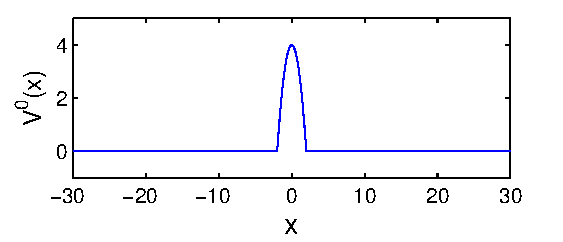
\includegraphics[width=0.8\textwidth]{Figures1/camdp/v1_mr.pdf}\\
\vspace{-2mm}
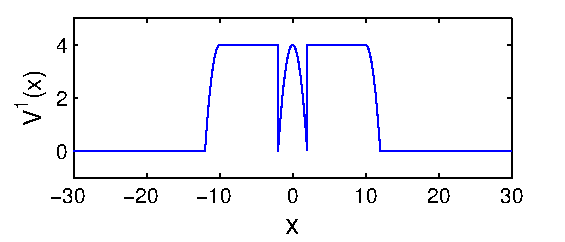
\includegraphics[width=0.8\textwidth]{Figures1/camdp/v2_mr.pdf}\\
\vspace{-2mm}
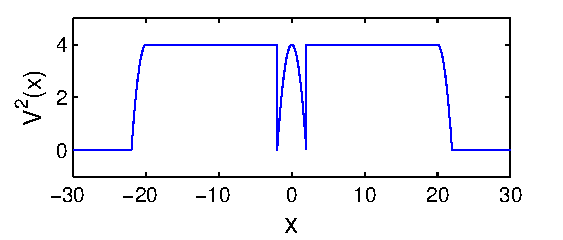
\includegraphics[width=0.8\textwidth]{Figures1/camdp/v3_mr.pdf}
\vspace{-3mm}

%\parbox{2.8in}{
\caption{\footnotesize Optimal sum of rewards (value) 
$V^t(x)$ for $b = 0 \, 
(\false)$ for time horizons (i.e., decision stages remaining) $t=0$,
$t=1$, and $t=2$ on the \textsc{Continuous Action}  \MarsRover\ problem.  For $x \in [-2,2]$, the
rover automatically takes a picture and receives a reward quadratic in
$x$.  We initialized $V^0(x,b) = R(x,b)$; for $V^1(x)$, the rover achieves
non-zero value up to $x = \pm 12$ and for 
$V^2(x)$, up to $x = \pm 22$.}
\label{fig:opt_graph}

\end{minipage}
%\end{figure}
%%%%%%%%%%%%%%%%%%%%%%%%%%%%%%%%%%%%%%%%%%%%%%%%%%%%%%%%%%%%%%%%%%%%%%%%%%
%%%%%%%%%%%%%%%%%%%%%%%%%%%%%%%%%%%%%%%%%%%%%%%%%%%%%%%%%%%%%%%%%%%%%%%%%%
%\begin{figure}[t!]
%\centering
%\subfigure{
%\hspace{-1mm}
\begin{minipage}[b]{0.53\linewidth}
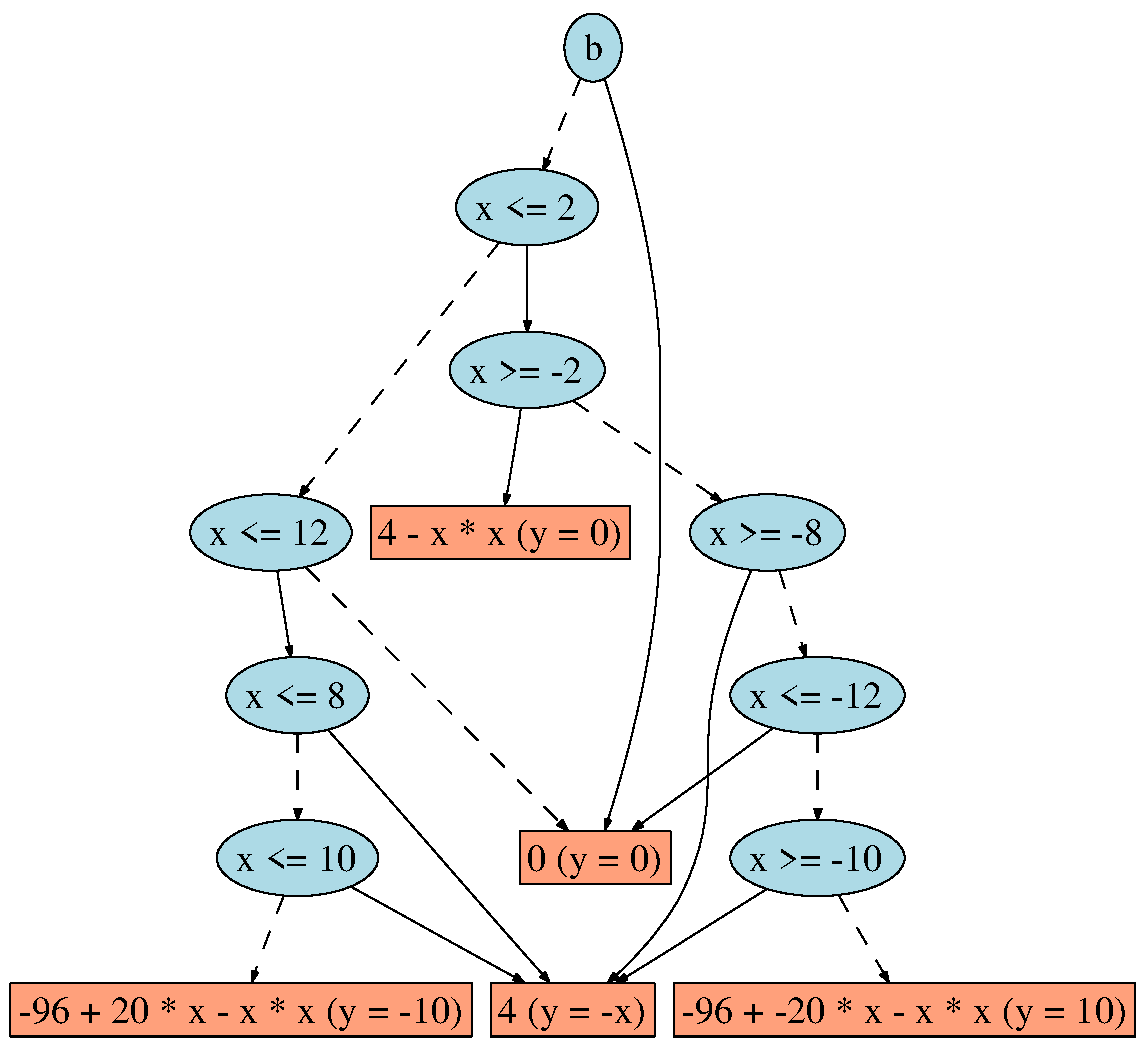
\includegraphics[width=0.9\textwidth]{Figures1/camdp/v2_mr_dd.pdf}
\vspace{2mm}

\caption{\footnotesize Optimal value function $V^1(x)$ for the
\textsc{Continuous Action}  \MarsRover\ problem represented as an extended algebraic decision
diagram (XADD).  Here the solid lines represent the $\true$ branch for
the decision and the dashed lines the $\false$ branch.  To evaluate
$V^1(x)$ for any state $x$, one simply traverses the diagram in a
decision-tree like fashion until a leaf is reached where the
non-parenthetical expression provides the \emph{optimal value} and the
parenthetical expression provides the \emph{optimal policy} 
($y = \pi^{*,1}(x)$) to achieve value $V^1(x)$.}
\label{fig:opt_val_pol}
\vspace{-5mm}
\end{minipage}
\vspace{-5mm}
\end{figure}
%%%%%%%%%%%%%%%%%%%%%%%%%%%%%%%%%%%%%%%%%%%%%%%%%%%%%%%%%%%%%%%%%%%%%%%%%%
If our objective is to maximize the long-term \emph{value} $V$ (i.e.,
the sum of rewards received over an infinite horizon of actions), then
we can write the optimal value achievable from a given state in \MarsRover\ 
as a function of state variables:
{%\footnotesize
%\begin{tabular}{l}
%$
\begin{align*}
V = \begin{cases}
\neg \mathit{take\-pic}_1 \land \mathit{take\-pic}_2 \land (4 -x^2 -y^2\geq 0) \land 
(5 - x^2 - y^2\geq 0) : & 4 -x^2 -y^2 \\
\mathit{take\-pic}_1 \land \neg \mathit{take\-pic}_2 \land (2 -x^2 -y^2\geq 0) \land 
(3 - x^2 - y^2\geq 0) : & 2 -x^2 -y^2 \\
\neg \mathit{take\-pic}_1 \land \mathit{take\-pic}_2 \land (4 -x^2 -y^2\geq 0) \land 
(5 - x^2 - y^2\leq 0) : & -1 \\
\mathit{take\-pic}_1 \land \neg \mathit{take\-pic}_2 \land (2 -x^2 -y^2\geq 0) \land 
(3 - x^2 - y^2\leq 0) : & -1 \\
else &: 0 \\
\end{cases} 
%$
%\end{tabular}
\end{align*}
}
The value function is piecewise and non-linear, and it contains non-rectangular decision
boundaries like $4 -x^2 -y^2\geq 0$. Figure ~\ref{fig:opt_graph} presents the  0-, 1-, and 2-step time horizon solutions for this problem; further, in symbolic form, we display both the 1-step time horizon value function and corresponding optimal policy in Figure ~\ref{fig:opt_val_pol}. Here, the piecewise nature of the transition and reward function leads to piece- wise structure in the value function and policy. Yet despite the intuitive and simple nature of this result, we are unaware of prior methods that can produce such exact solutions. 

\paragraph{\WaterReservoir} 
Reservoir management is well-studied in
the OR literature \cite{Mahootchi2009,Yeh1985}.  The key continuous decision is how
much elapsed time $e$ to
\emph{drain} (or \emph{not drain}) each reservoir to maximize
electricity revenue over the decision-stage horizon while avoiding
reservoir overflow and underflow.  Cast as a CA-HMDP, we 
believe SVI provides the first approach capable of deriving
an exact closed-form non-myopic optimal policy
for all levels.

We examine a 2-reservoir problem with
respective levels $(l_1,l_2)\in [0,\infty]^2$ with reward penalties for 
overflow and underflow and a reward gain linear in the elapsed time $e$ for
electricity generated in periods when the $\mathit{drain}(e)$ action
drains water from $l_2$ to $l_1$ (the other action is 
$\mathit{no}$-$\mathit{drain}(e)$); we assume deterministic rainfall
replenishment and present the reward function as:  

\vspace{-4mm}
{\footnotesize
\begin{align*}
R & = \begin{cases}
((50-200*e) \leq l_1 \leq (4500-200*e)) \wedge ((50+100*e) \leq l_2 \leq (4500+100*e)) %\\ \hspace{4mm} \vspace{3mm} 
&:e\\
((50+300*e) \leq l_1 \leq (4500+300*e)) \wedge ((50-400*e) \leq l_2 \leq (4500-400*e)) %\\ \hspace{4mm} \vspace{3mm} 
&:0\\
\text{\normalsize otherwise} &: -\infty \\
\end{cases}
\end{align*}}
The transition function for levels of the $\mathit{drain}$ action is defined below. Note that for the $\mathit{no}$-$\mathit{drain}$ action, the $\mathit{500 * e}$ term is not involved.
{%\footnotesize 
\begin{align*}
l_1' & =(400 * e + l_1 -700 * e + 500 * e) \\
l_2'& =(400 * e + l_2 - 500 * e) \\
\end{align*}}

Similar to the discrete version of the \InventoryControl problem in the introduction, the DA-HMDP setting for these two problems defines discrete actions by partitioning the action space of each domain into 1/10 slices. For the \MarsRover\ problem this defines 2 actions ($a_1=[-10,0], a_2 = [0,10]$), for \WaterReservoir  the discrete time action set is a set of 20 elements where $e_1=[0,10]$ and $e_20 = [190,200]$ and the transition and reward functions are defined according to these constant values.
We now provide the empirical results obtained from implementing our algorithms.

\subsection{Results}

For the \textsc{Discrete Action} \MarsRover\ domains, 
we have run experiments to evaluate our SDP solution 
in terms of time and space cost while varying the horizon and problem size.

Because the reward and transition functions for \textsc{Discrete Action}  \MarsRoverL\ use piecewise linear case statements, we note the optimal value function
in this domain is also piecewise linear.  Hence in this domain, we use
a linear constraint feasibility checker to prune unreachable paths in
the XADD, we also compare solutions for \MarsRover with and
without this pruning.
%%%%%%%%%%%%%%%%%%%%%%%%%%%%%%%%%%%%%%%%%%%%%%%%%%%%%%%%%%%%%%%%%%%%%%%%%%
%\begin{figure*}[t]
%\centering
%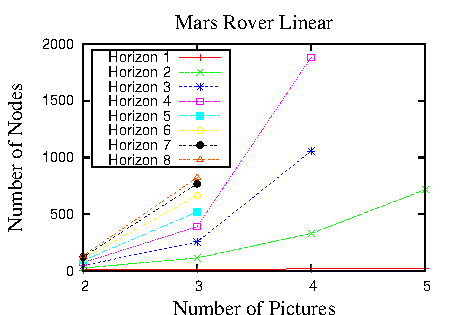
\includegraphics[width=0.42\textwidth]{Figures1/cmdp/SpaceVsPictureLinear.pdf}
%\hspace{5mm}
%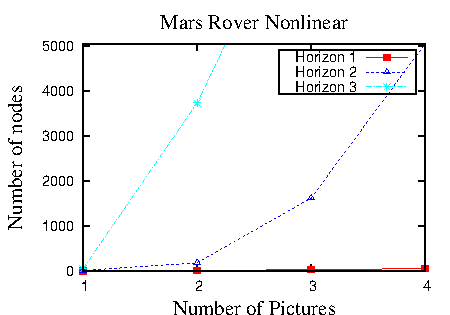
\includegraphics[width=0.42\textwidth]{Figures1/cmdp/SpaceVsPictures.pdf}
%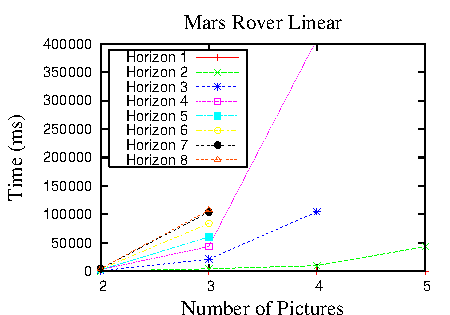
\includegraphics[width=0.42\textwidth]{Figures1/cmdp/TimeVsPicturesLinear.pdf}
%\hspace{5mm}
%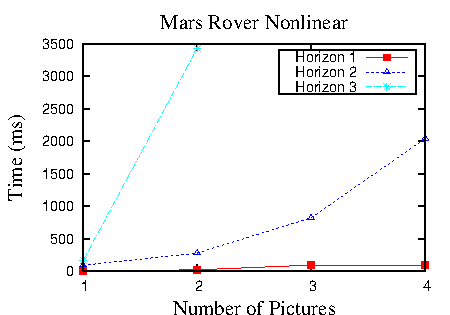
\includegraphics[width=0.42\textwidth]{Figures1/cmdp/TimeVsPictures.pdf}
%\caption{%\footnotesize 
%Space (\# XADD nodes in value function) 
%and time to optimally solve different problem 
%sizes of the two \textsc{Discrete Action}  \MarsRover~domains for varying horizon lengths.}
%\label{fig:all_lin}
%\vspace{-5mm}
%\end{figure*}
%%%%%%%%%%%%%%%%%%%%%%%%%%%%%%%%%%%%%%%%%%%%%%%%%%%%%%%%%%%%%%%%%%%%%%%%%%
%In Figure~\ref{fig:all_lin}, for both the \textsc{Discrete Action}  \MarsRoverL\ and \textsc{Discrete Action}  \MarsRoverNL\ domains, we show how the number of nodes of the value function XADD (proportional to the space required to represent the value function) varies for each iteration (horizon) and different problem sizes (given by the number of pictures).  We first note that the nonlinear variant appears \emph{much} harder for SDP (much more time required and larger value functions) than for the linear variant --- this is largely due to the fact that the XADD can be optimally pruned in the linear variant.  Secondly, we note an apparent superlinear growth in space and time required to solve each problem as a function of the number of picture points --- this likely reflects the superlinear growth of combinations of pictures that must be jointly considered as the number of pictures increases.  Finally, from these graphs it is hard to summarize general algorithm behavior as a function of horizon, but it appears for the linear problem variant that both the time  and space grow linearly as a function of horizon --- this will be confirmed in the next experiments.  

%Figure~\ref{fig:lin3} shows the amount of time for each iteration of SDP vs. horizon for \MarsRoverL\ with three picture points for SDP with and without XADD pruning.  Here we see an impressive reduction in time and space as a function of horizon with pruning.  Without pruning, both time and space grow super-linearly with the horizon, while with pruning time and space appear to grow linearly with the horizon.
%%%%%%%%%%%%%%%%%%%%%%%%%%%%%%%%%%%%%%%%%%%%%%%%%%%%%%%%%%%%%%%%%%%%%%%%%%
%\begin{figure*}[t]
%\centering
%%\subfigure{
%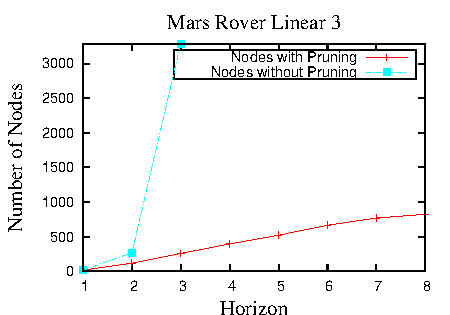
\includegraphics[width=0.4\textwidth]{Figures1/cmdp/SpaceVsHorizonRoverLinear3.pdf}
%\hspace{5mm}
%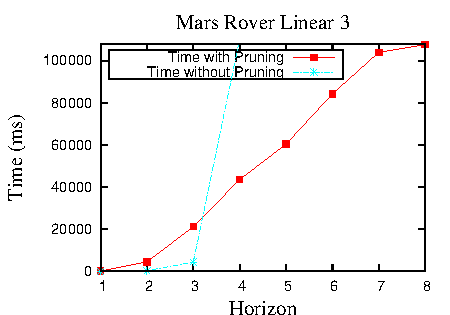
\includegraphics[width=0.4\textwidth]{Figures1/cmdp/TimeVsHorizonRoverLinear3.pdf}
%%}
%%\vspace{-3mm}
%\caption{%\footnotesize 
%Space (\# XADD nodes in value function) and
%time for different iterations (horizons) of SDP on \textsc{Discrete Action} \MarsRoverL\ 
%with 3 image target points.  Results shown for SDP with and without XADD 
%infeasible path pruning.}
%\label{fig:lin3}
%\vspace{-3mm}
%\end{figure*}
%%%%%%%%%%%%%%%%%%%%%%%%%%%%%%%%%%%%%%%%%%%%%%%%%%%%%%%%%%%%%%%%%%%%%%%%%%
%%%%%%%%%%%%%%%%%%%%%%%%%%%%%%%%%%%%%%%%%%%%%%%%%%%%%%%%%%%%%%%%%%%%%%%%%%
%\begin{figure*}[t]
%\centering
%%\subfigure{
%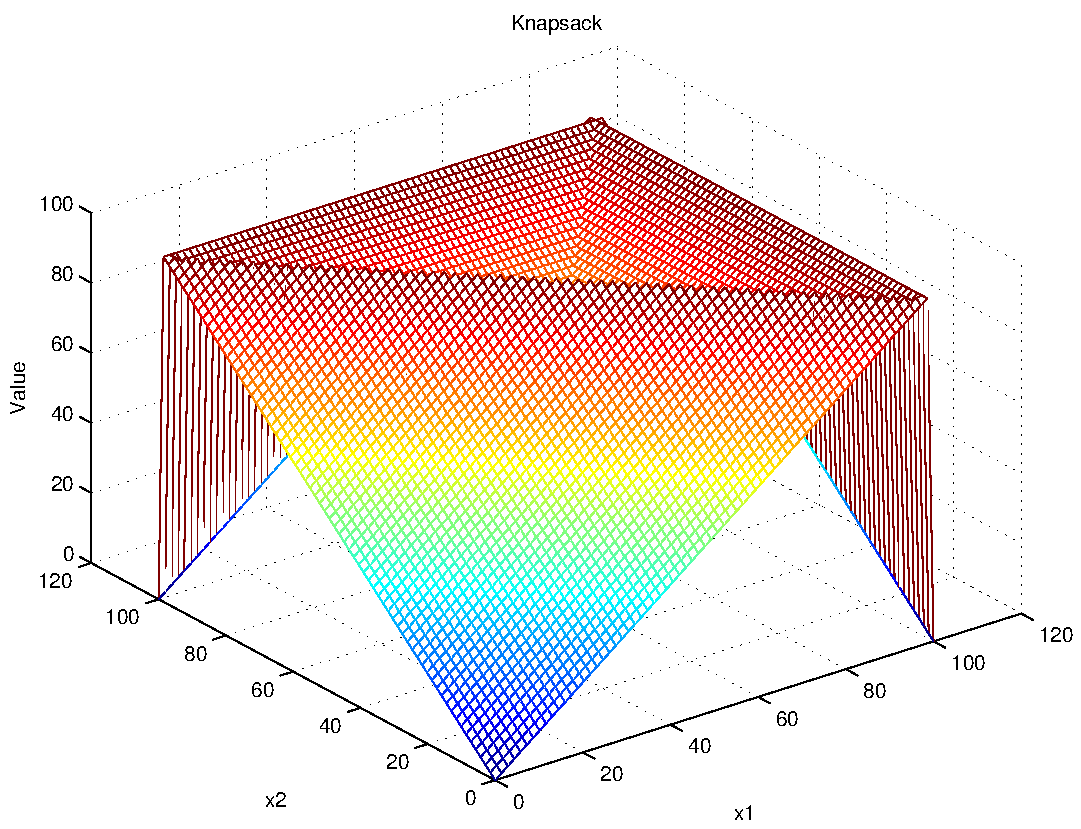
\includegraphics[width=0.31\textwidth]{Figures1/cmdp/Knapsack.pdf}
%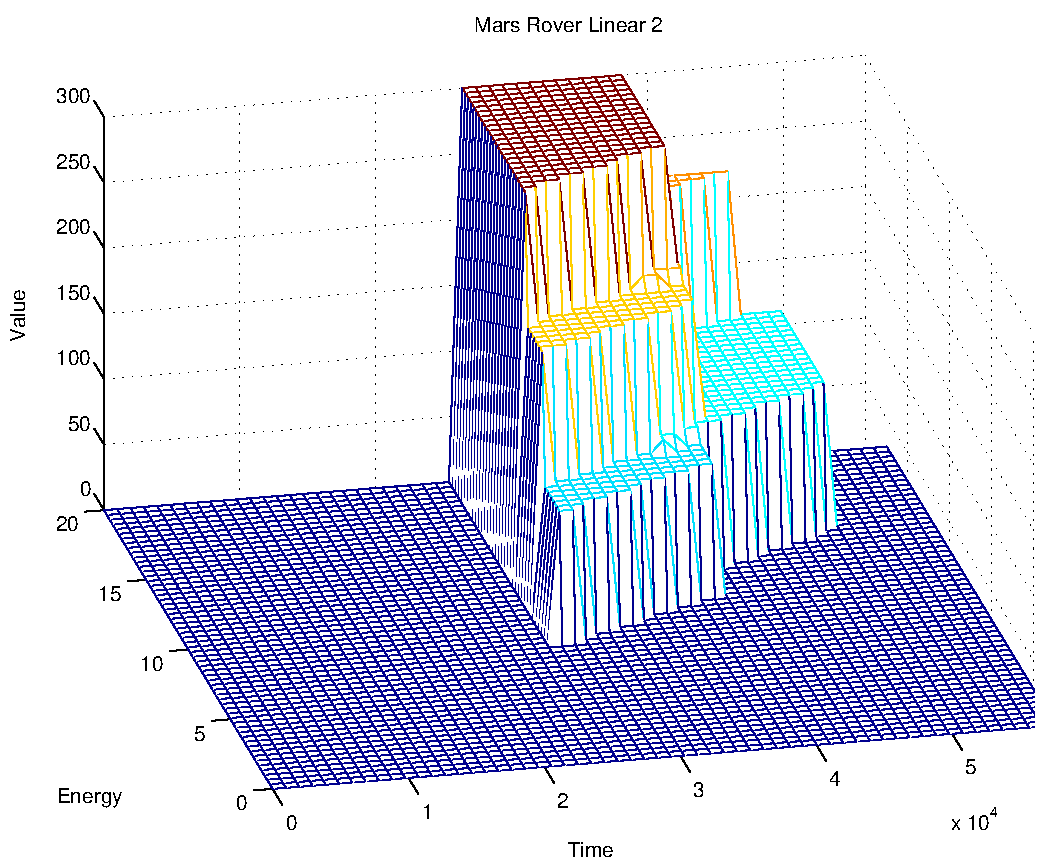
\includegraphics[width=0.31\textwidth]{Figures1/cmdp/MarsRoverLinear2.pdf}
%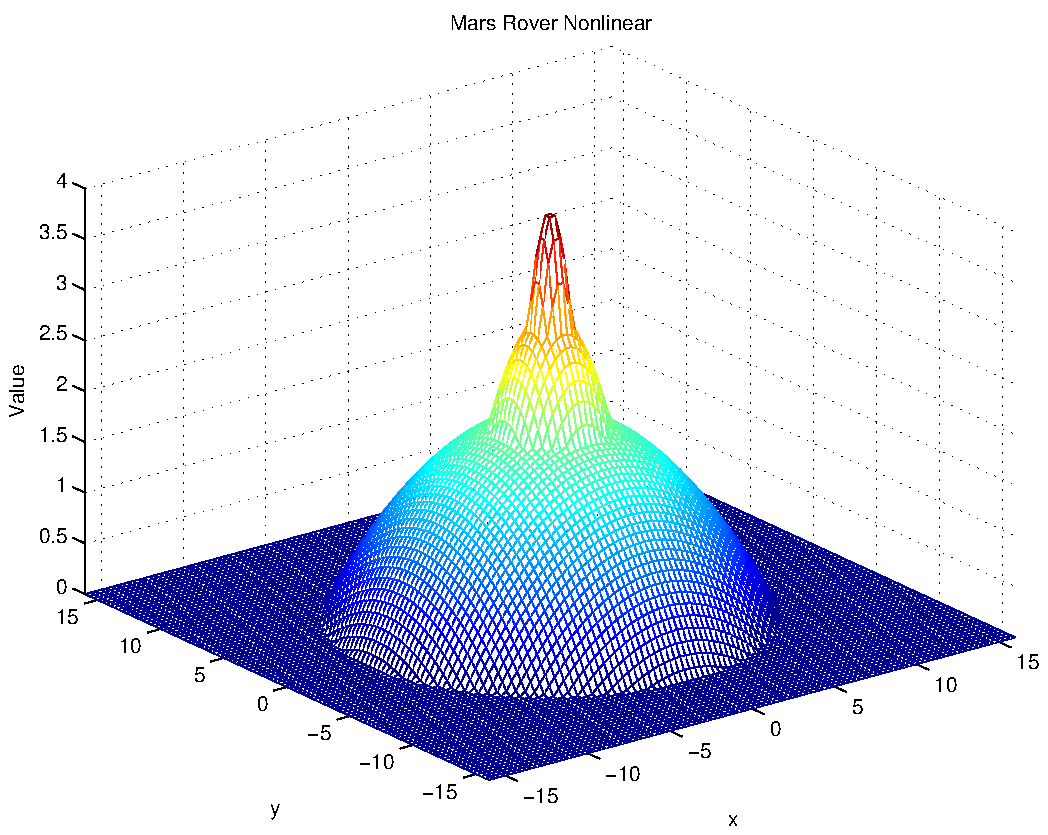
\includegraphics[width=0.31\textwidth]{Figures1/cmdp/MarsNonlinear.pdf}
%%}
%%\vspace{-3mm}
%\caption{%\footnotesize 
%\emph{Optimal} value function (vertical axis) for different domains showing 
%\emph{non-rectangular} piecewise boundaries.  From left to right, \Knapsack\ 
%($H = \infty$, horizontal axes $x_2$ and $x_1$),
%\MarsRoverL\ with two pictures ($H = 8$, horizontal axes $\mathit{energy}$ and 
%$\mathit{time}$), and \MarsRoverNL\ with one picture ($H = 3$, horizontal axes 
%$y$ and $x$).}
%\label{fig:plot3D}
%\vspace{-5mm}
%\end{figure*}
%%%%%%%%%%%%%%%%%%%%%%%%%%%%%%%%%%%%%%%%%%%%%%%%%%%%%%%%%%%%%%%%%%%%%%%%%%
%In Figure~\ref{fig:plot3D}, we show the exact optimal value function on the vertical axis  for three domains, \Knapsack\, \textsc{Discrete Action}  \MarsRoverL ~and \textsc{Discrete Action}  \MarsRoverNL, as a function of two continuous state variables shown on the horizontal axes.
We notice here that the piecewise boundaries for all three
plots clearly demonstrate non-rectangular boundaries. In particular, the
value function plot for the \MarsRover demonstrates nonlinear
piecewise boundaries with each piece being a nonlinear function of the
state --- it has the shape of stacked quadratic cones with each lower
cone representing the cost of first moving from points farther away
from the picture being receiving the value for taking the picture
within the radius limits.

%%%%%%%%%%%%%%%%%%%%%%%%%%%%%%%%%%%%%%%%%%%%%%%%%%%%%%%%%%%%%%%%%%%%%%%%%%
\begin{figure*}[t]
\centering
%\subfigure{
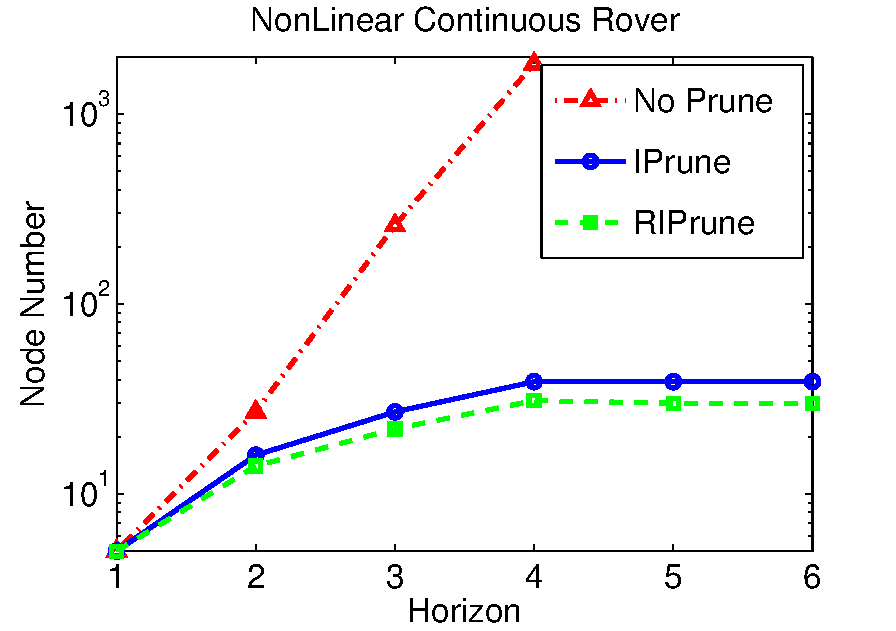
\includegraphics[width=0.4\textwidth]{Figures1/camdp/nodeRover.pdf}
\hspace{5mm}
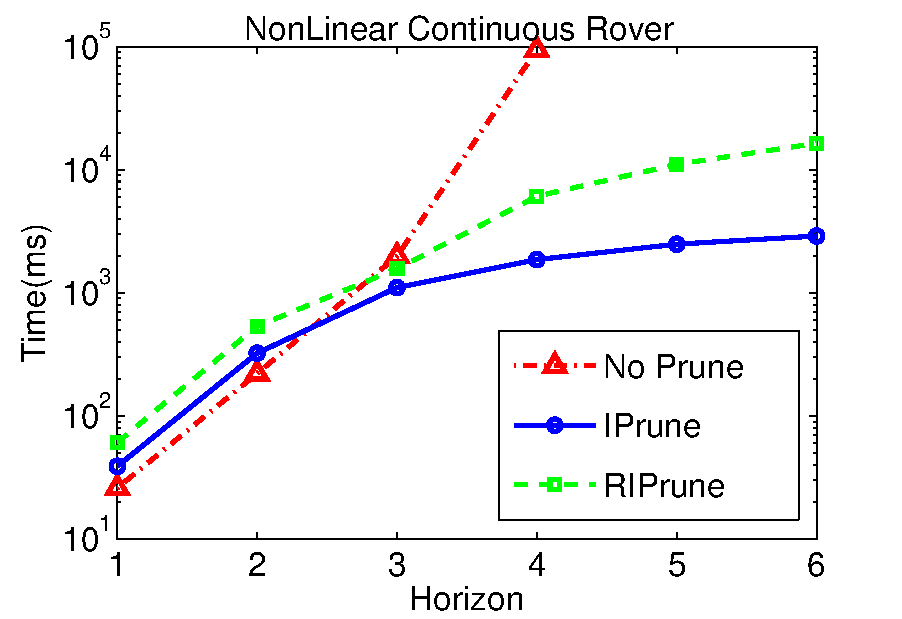
\includegraphics[width=0.4\textwidth]{Figures1/camdp/timeRover.pdf}
%}
\vspace{-3mm}
\caption{%\footnotesize 
Space (\# XADD nodes in value function) and
time for different iterations (horizons) of SDP on Nonlinear \textsc{Continuous Action}  \MarsRover\ with 3 different results based on pruning techniques. Results are shown for  the XADD 
 with no pruning technique, with only inconsistency checking (using LP-solver) and with both the inconsistent and redundancy checking (using LP-Solver and SAT-Solver).}
\label{fig:roverTS}
\vspace{-6mm}
\end{figure*}
%%%%%%%%%%%%%%%%%%%%%%%%%%%%%%%%%%%%%%%%%%%%%%%%%%%%%%%%%%%%%%%%%%%%%%%%%%
%%%%%%%%%%%%%%%%%%%%%%%%%%%%%%%%%%%%%%%%%%%%%%%%%%%%%%%%%%%%%%%%%%%%%%%%%%
%figure5 : time-iteration and space-iteraton for 1d-2d-noPrune inventory
\begin{figure}[tbp!]
\vspace{-2mm}
\centering
%\subfigure{
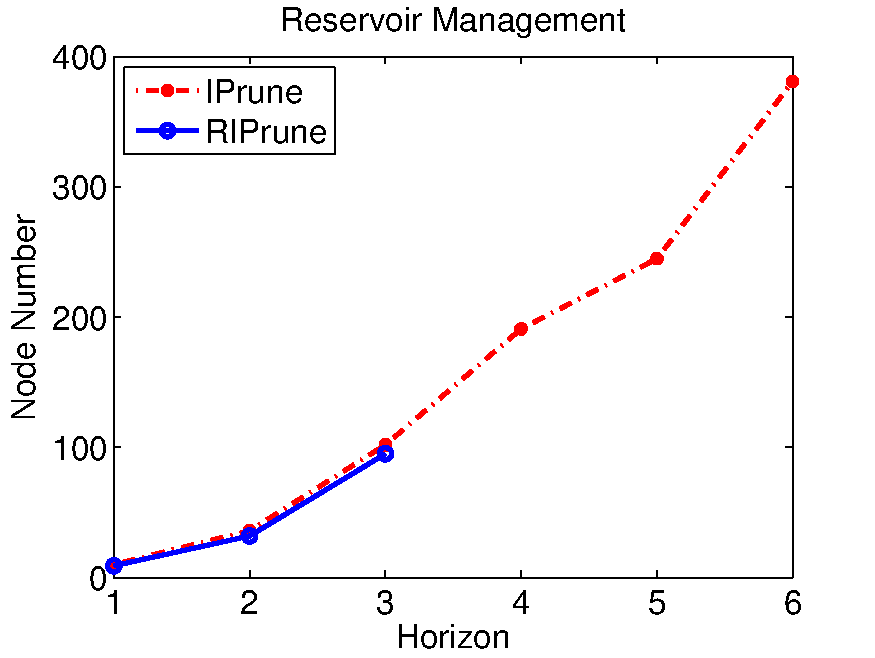
\includegraphics[width=0.45\textwidth]{Figures1/camdp/ResNode.pdf}
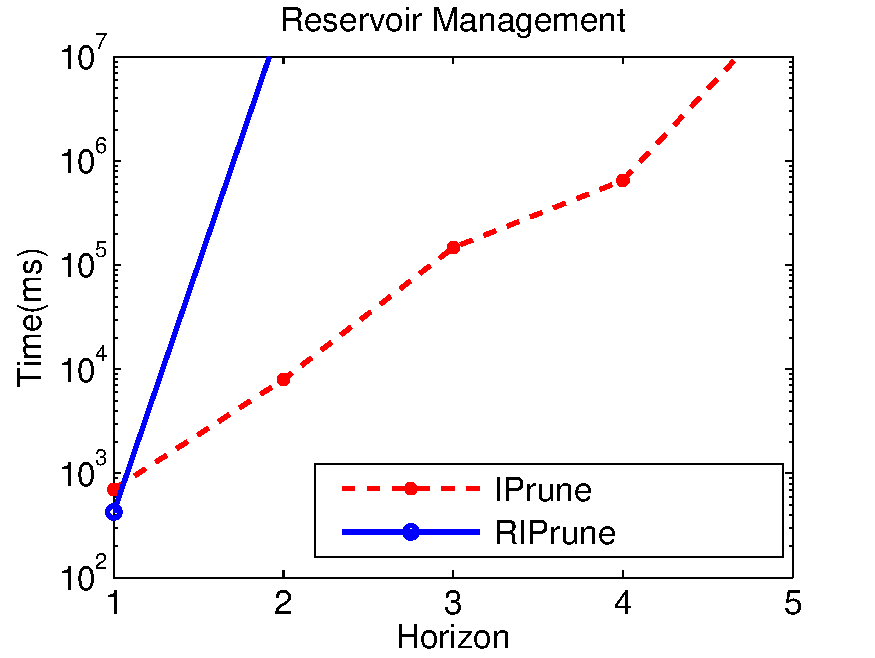
\includegraphics[width=0.45\textwidth]{Figures1/camdp/ResTime.pdf}
%}
\vspace{-2mm}
\caption{%\footnotesize 
Reservoir Management: space and elapsed time vs. horizon. Comparing the two algorithms for inconsistency pruning (IPrune) and redundancy and inconsistency pruning (RIPrune).  
% comparing 
%1,2 or 3 States and actions (SA) with Deterministic (DD) 
%or Stochastic (SD) demand and no-pruning}.
}
\label{fig:resTimeSpace}
\vspace{-5mm}
\end{figure}
%%%%%%%%%%%%%%%%%%%%%%%%%%%%%%%%%%%%%%%%%%%%%%%%%%%%%%%%%%%%%%%%%%%%%%%%%%
To the best of our knowledge, these results demonstrate the first
exact analytical solutions for HMDPs having optimal value functions
with general linear and even nonlinear piecewise boundaries.

For the \textsc{Continuous Action} \MarsRover problem, we present the time and space analysis for the problem description defined in the introduction in Figure~\ref{fig:roverTS}. Here three evaluations are performed based on the pruning algorithms in the previous section. We note that without the LP-Solver Algorithm~\ref{algPrune}, the algorithm can not go beyond the forth iteration as it produces many inconsistent nodes. For the redundancy check of Algorithm~\ref{algRedundant}, as it can be seen in the graph, a reduction of at most 25 \% is achieved. The time required to remove redundancy has increased due to the calls made to the SAT-Solver.  

Figure ~\ref{fig:resTimeSpace} compares inconsistency pruning and redundancy pruning for the reservoir management problem. In this setting, very little node reduction can be gained from redundancy pruning due to the different water levels and their correlation. The time has increased rapidly after the second iteration for the redundancy pruning due to the equivalence checking of the SAT-Solver. This suggests that in some domains using redundancy pruning in not efficient and should be omitted from the final results. We next show results for the \InventoryControl problem without redundancy pruning. 

In Figure~\ref{fig:v2plots}, we show a plot of 
the optimal closed-form policy at $h=2$: the solution interleaves $\mathit{drain}(e)$ and $\mathit{no}$-$\mathit{drain}(e)$ where even horizons are the latter;
here we see that we avoid draining for the longest elapsed time $e$ 
when $l_2$ is low (wait for rain to replenish) and $l_1$ is high (draining
water into it could overflow it).  $V^2(l_1,l_2)$ and $V^9(l_1,l_2)$
show the progression of convergence from horizon $h=2$ to $h=9$ ---
low levels of $l_1$ and $l_2$ allow the system to generate electricity
for the longest total elapsed time over 9 decision stages. 
%%%%%%%%%%%%%%%%%%%%%%%%%%%%%%%%%%%%%%%%%%%%%%%%%%%%%%%%%%%%%%%%%%%%%%%%%%
% policy2, v2plot.pdf, v9plot
% annotation?
\begin{figure*}[tbp!]
\vspace{-2mm}
\centering
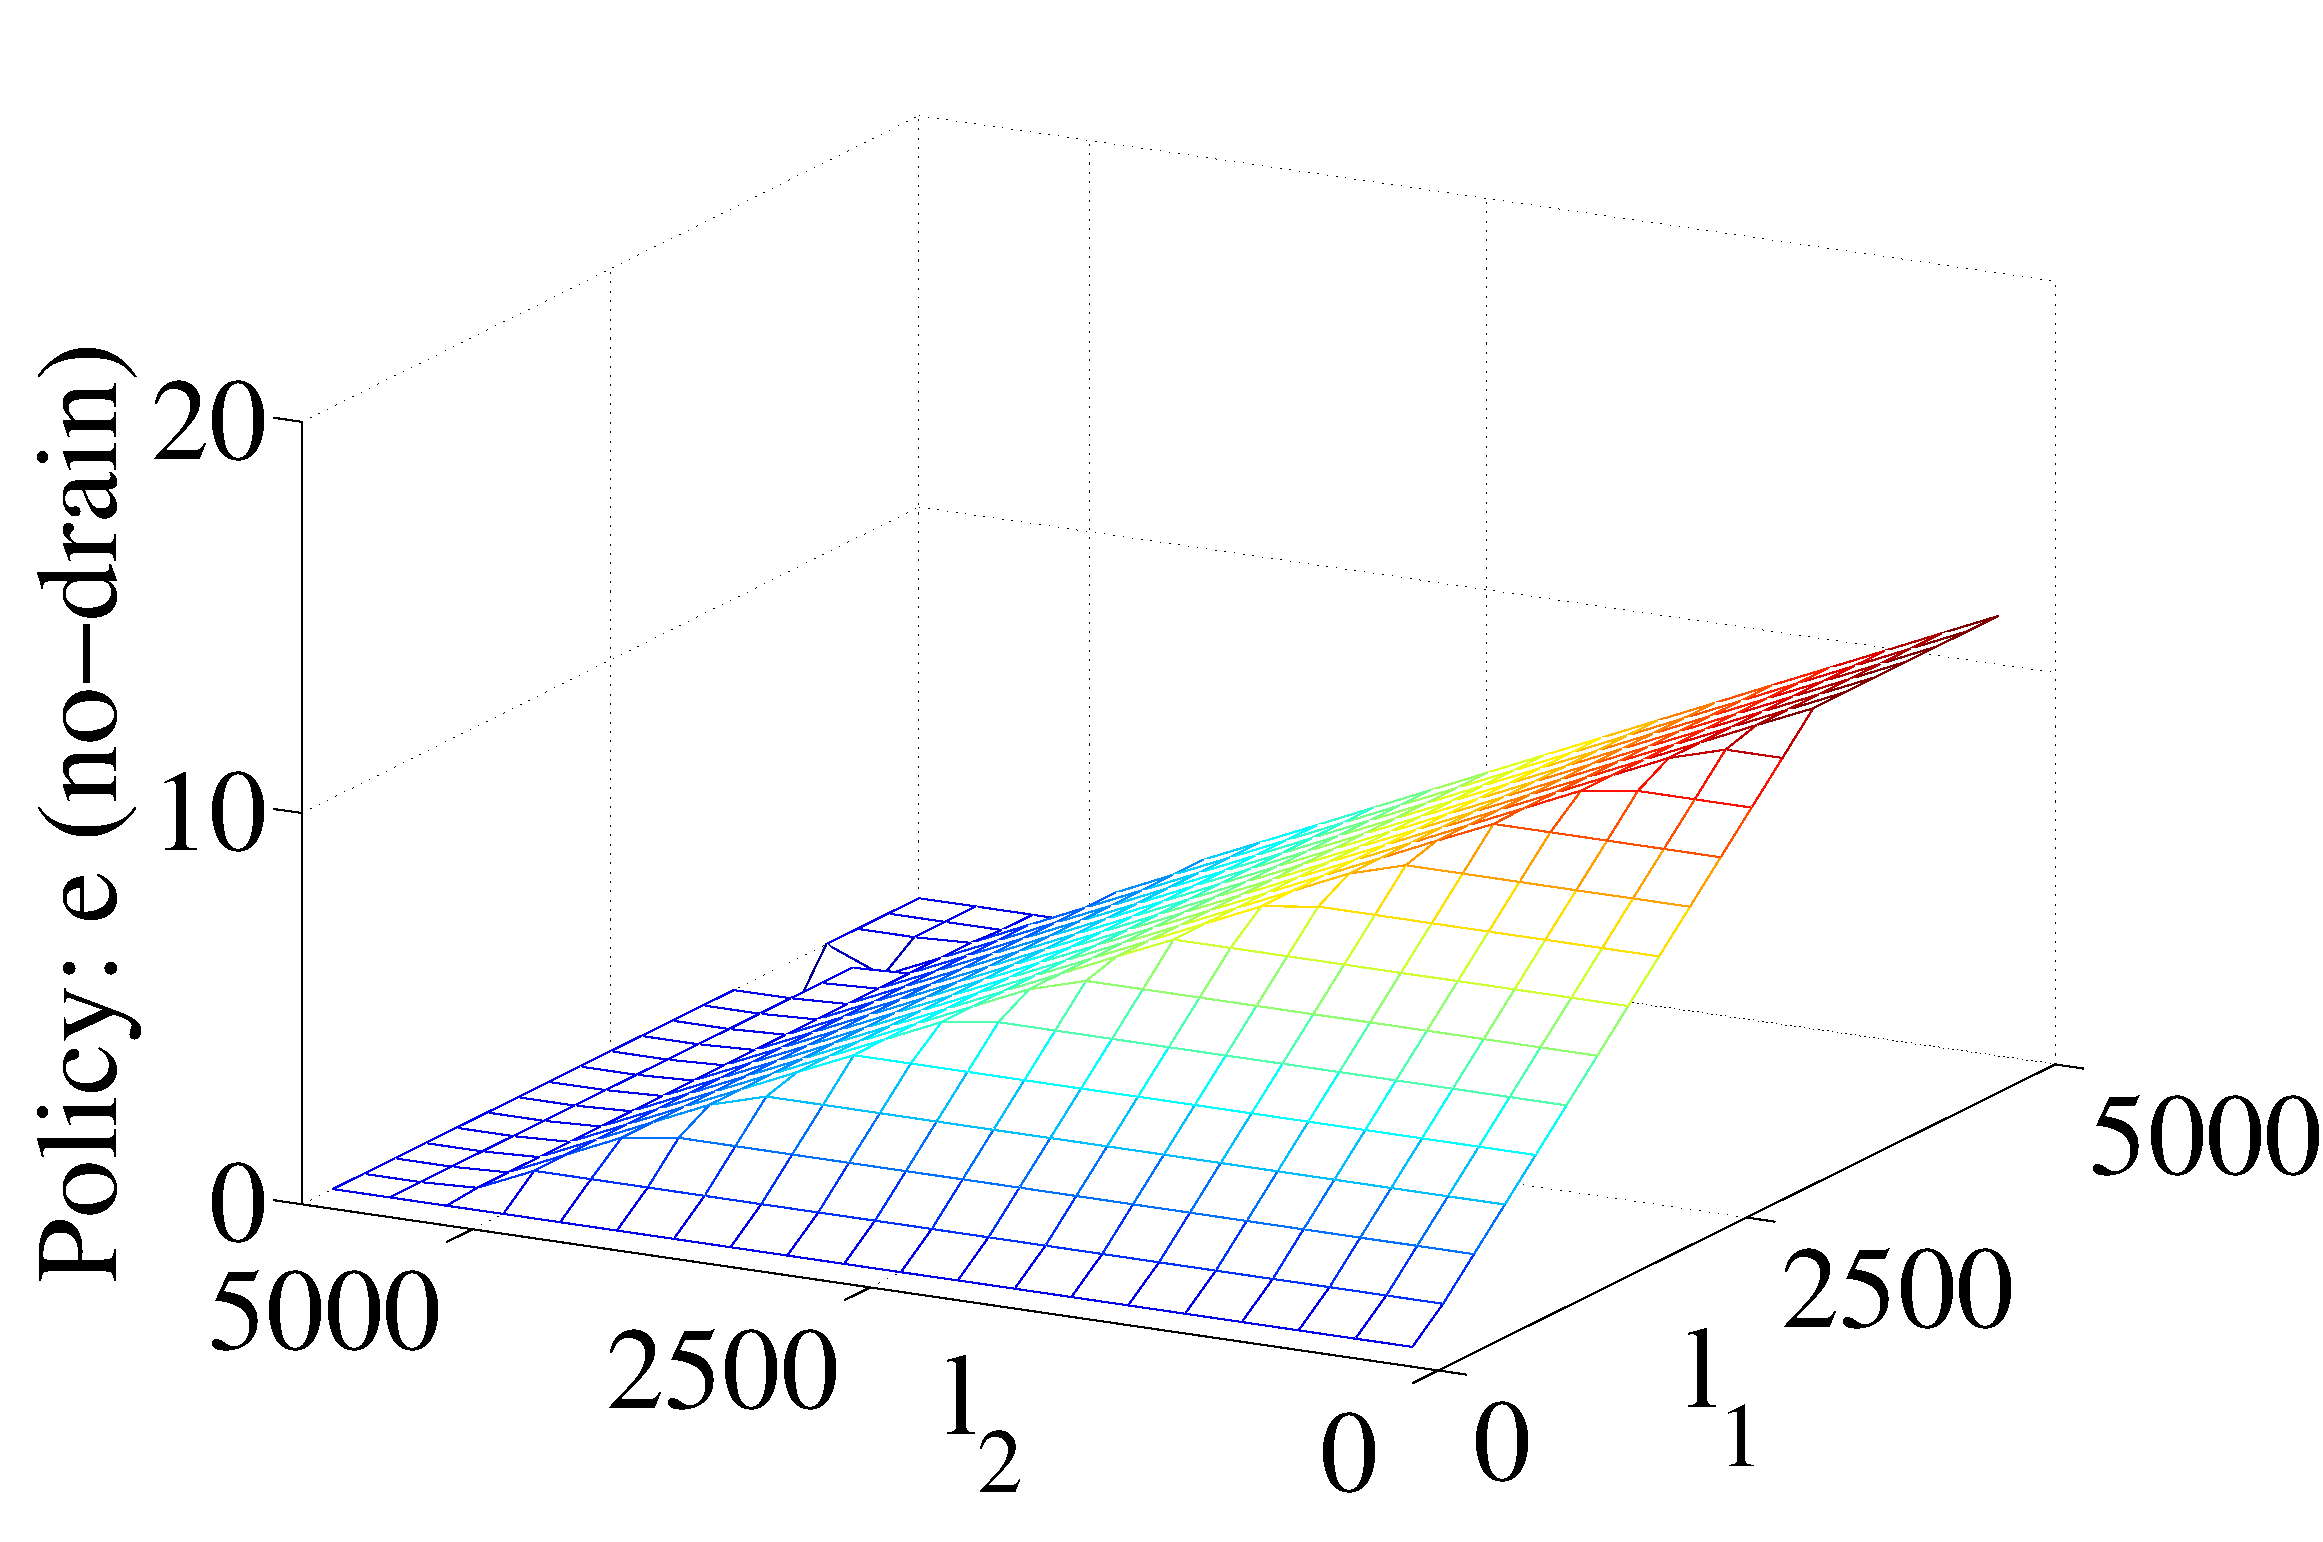
\includegraphics[width=0.3\textwidth]{Figures1/camdp/policy-iteration2-3.pdf}
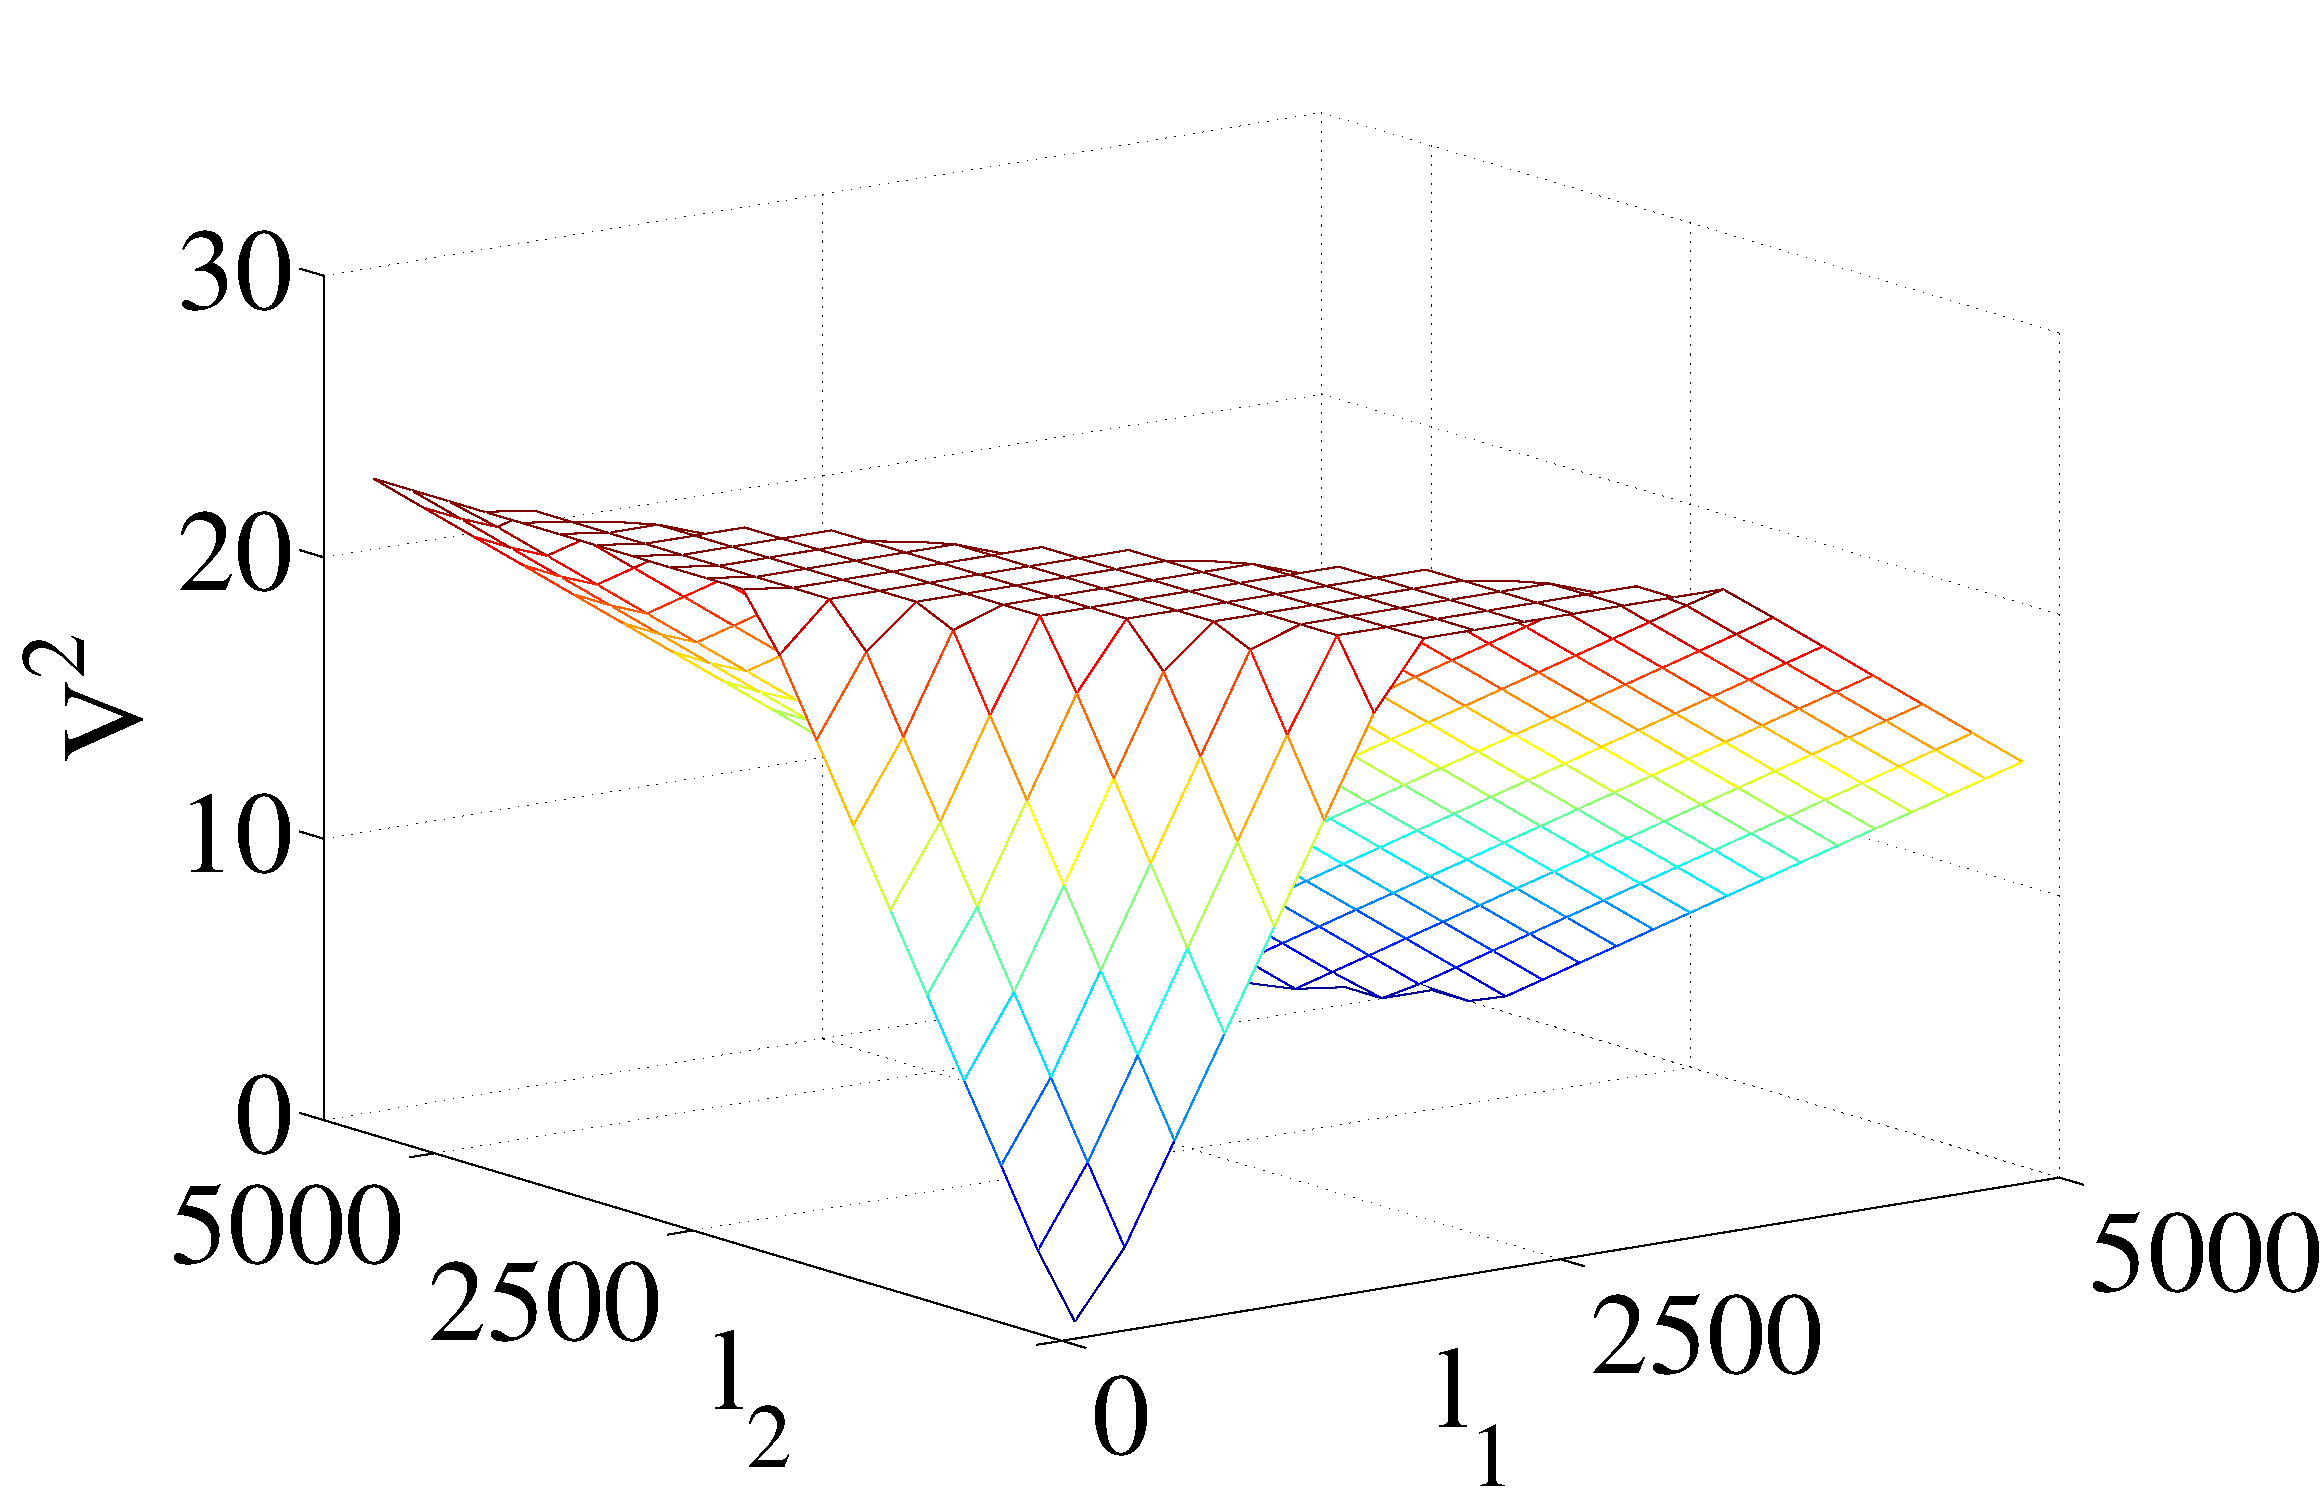
\includegraphics[width=0.3\textwidth]{Figures1/camdp/V2.pdf}
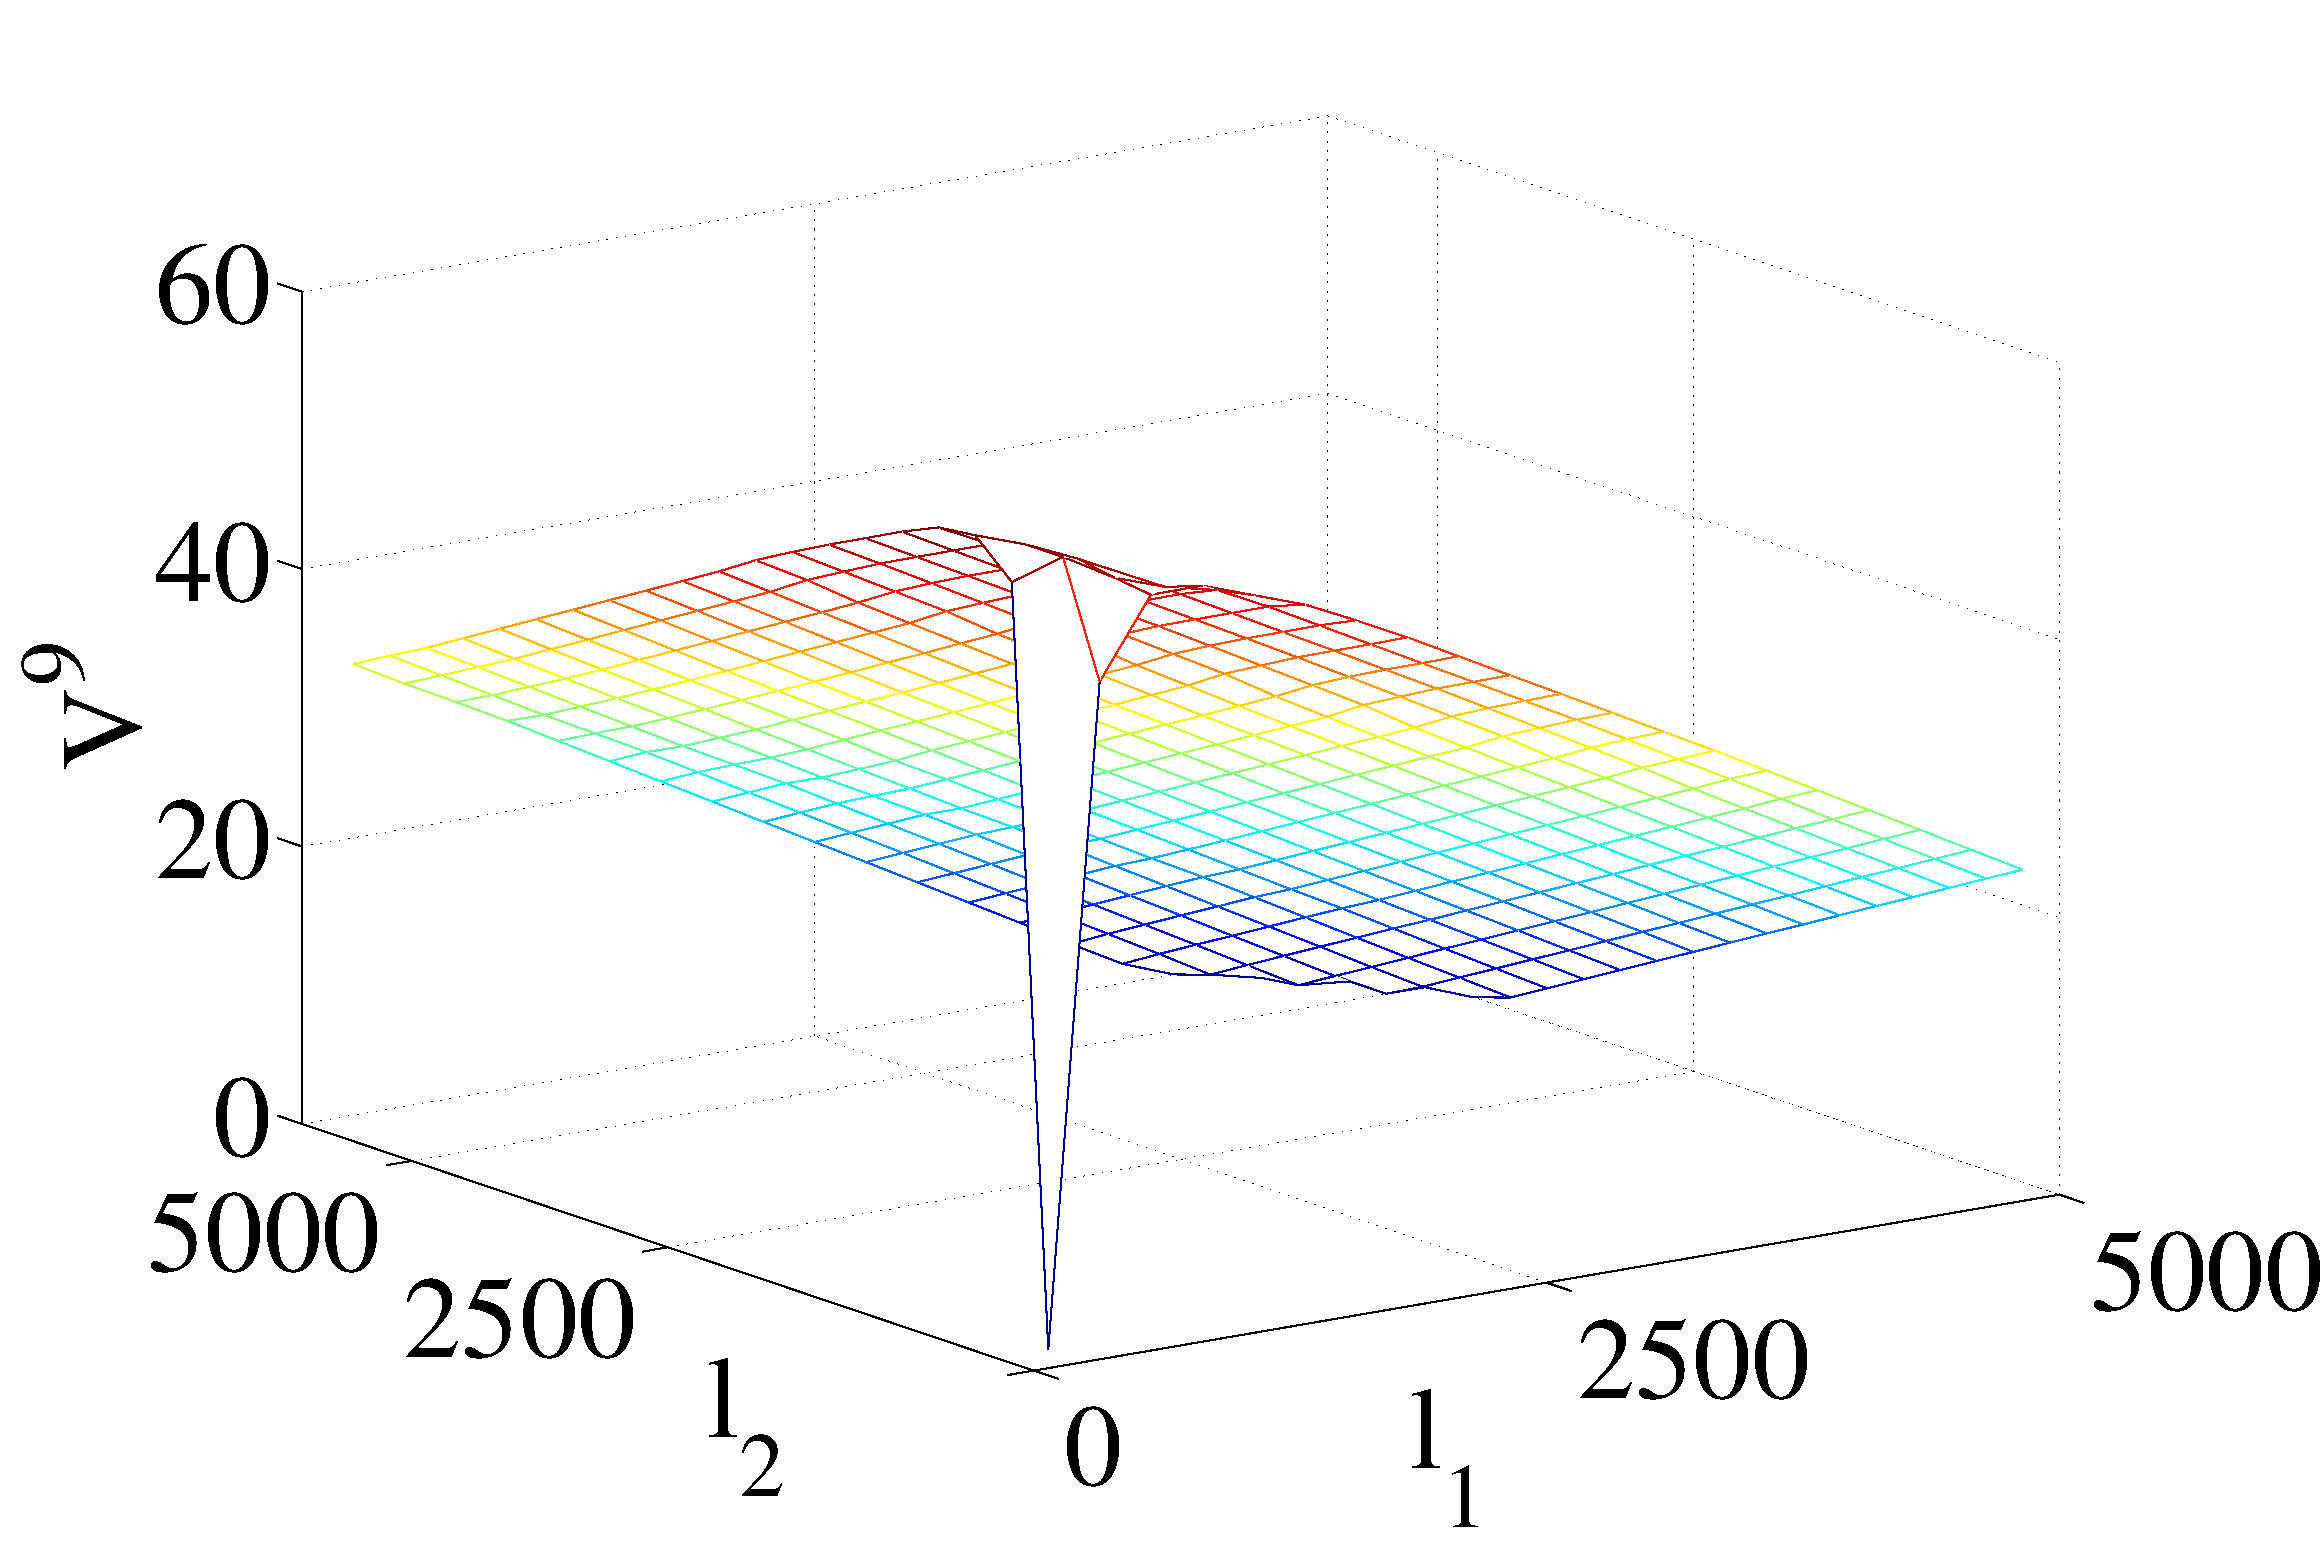
\includegraphics[width=0.3\textwidth]{Figures1/camdp/V9.pdf}
\vspace{-3mm}
\caption{%\footnotesize 
\WaterReservoir: 
{\it (left)} Policy $\mathit{no}$-$\mathit{drain}(e)=\pi^{2,*}(l_1,l_2)$ 
showing on the z-axis the elapsed time $e$ that should be executed 
for $\mathit{no}$-$\mathit{drain}$ conditioned on the states; 
{\it (middle)} $V^2(l_1,l_2)$; 
{\it (right)} $V^9(l_1,l_2)$.
}
\label{fig:v2plots}
\vspace{-4mm}
\end{figure*}
%%%%%%%%%%%%%%%%%%%%%%%%%%%%%%%%%%%%%%%%%%%%%%%%%%%%%%%%%%%%%%%%%%%%%%%%%% 
%%%%%%%%%%%%%%%%%%%%%%%%%%%%%%%%%%%%%%%%%%%%%%%%%%%%%%%%%%%%%%%%%%%%%%%%%%
%figure5 : time-iteration and space-iteraton for 1d-2d-noPrune inventory
\begin{figure}[tbp!]
\vspace{-2mm}
\centering
%\subfigure{
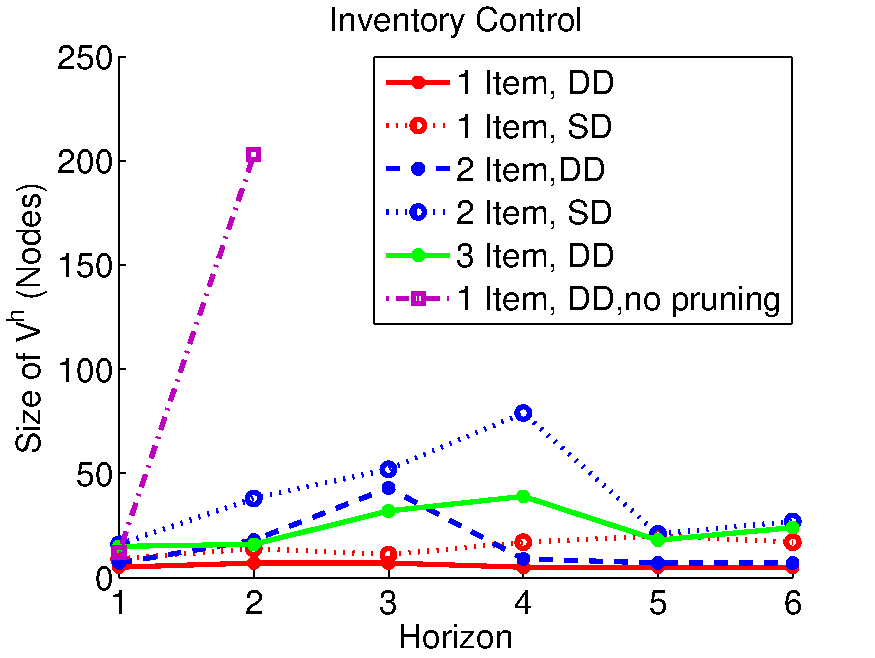
\includegraphics[width=0.45\textwidth]{Figures1/camdp/inventorySpace.pdf}
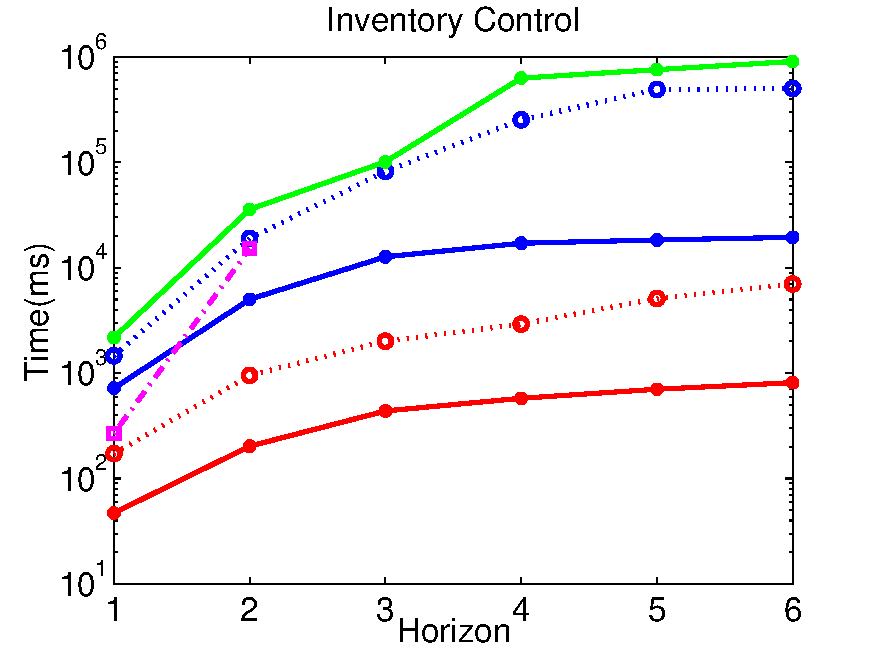
\includegraphics[width=0.45\textwidth]{Figures1/camdp/inventoryTime.pdf}
%}
\vspace{-2mm}
\caption{%\footnotesize 
\InventoryControl: space and time vs. horizon.
% comparing 
%1,2 or 3 States and actions (SA) with Deterministic (DD) 
%or Stochastic (SD) demand and no-pruning}.
}
\label{fig:invC}
\vspace{-2mm}
\end{figure}
%%%%%%%%%%%%%%%%%%%%%%%%%%%%%%%%%%%%%%%%%%%%%%%%%%%%%%%%%%%%%%%%%%%%%%%%%%

In Figure~\ref{fig:invC}, we provide a time and space analysis of
deterministic- and stochastic-demand (resp. DD and SD) variants of the
SCIC and MJCIC problem for up to three items (the same scale of
problems often studied in the OR literature); for each number of items
$n \in \{ 1,2,3 \}$ the state (inventory levels) is $\vec{x} \in
[0,\infty]^n$ and the action (reorder amounts) is $\vec{y} \in
[0,\infty]^n$.  Orders are made at one month intervals and we solve
for a horizon up to $h=6$ months.  Here we see that linear feasibility
checking/pruning in the XADD is crucial -- we cannot solve beyond
$h=2$ without it for 1 item!  While solving for larger numbers of
items and SD (rather than DD) both increase time and space, 
the solutions quickly reach quiescence indicating structural
convergence.

%\vspace*{-0.05in}
\section{Related Work}

The most relevant vein of related work for DA-HMDPs is that of \cite{feng04} and \cite{li05} which can perform exact dynamic programming on
HMDPs with rectangular piecewise linear reward and transition functions
that are delta functions.  While SDP can solve these same problems,
it removes both the rectangularity and piecewise restrictions on the
reward and value functions, while retaining exactness.  
Heuristic search approaches with formal guarantees 
like HAO* \cite{hao09} are an attractive future extension of SDP;
in fact HAO* currently uses the method of \cite{feng04}, which could
be directly replaced with SDP.  While \cite{penberthy94} has considered
general piecewise functions with linear boundaries (and in fact,
we borrow our linear pruning approach from this paper), this work
only applied to fully deterministic settings, not HMDPs.

Other work has analyzed limited HMDPS having only one continuous
state variable.  Clearly rectangular restrictions are meaningless with
only one continuous variable, so it is not surprising that more
progress has been made in this restricted setting.  One continuous
variable can be useful for optimal solutions to time-dependent MDPs 
(TMDPs) \cite{boyan01}.  Or phase transitions can be used to 
arbitrarily approximate one-dimensional continuous distributions
leading to a bounded approximation approach for arbitrary single continuous
variable HMDPs \cite{phase07}.  
While this work cannot handle arbitrary stochastic
noise in its continuous distribution, it does exactly solve HMDPs
with multiple continuous state dimensions.

There are a number of general HMDP approximation
approaches that use approximate linear programming \cite{kveton06}
or sampling in a reinforcement learning style approach \cite{munos02}.
In general, while approximation methods are quite promising in
practice for HMDPS, the objective of this paper was to push
the boundaries of \emph{exact} solutions; however, in some sense, 
we believe that more expressive exact solutions may also inform
better approximations, e.g., by allowing the use of data structures
with non-rectangular piecewise partitions that allow higher fidelity
approximations.

%As for continuous actions and states, there has been prior work on approximate solutions to continuous state MDPs \cite{munos02,phase07} and even continuous state and action
%MDPs \cite{kveton06}, which might inform future approximate extensions
%of this work.  
As for CA-HMDPs, there has been prior work in control theory. The field of linear-quadratic Gaussian (LQG) control \cite{lqgc} which use linear dynamics with continuous actions, Gaussian noise, and quadratic
reward is most closely related.  However, these exact solutions do
not extend to discrete and continuous systems with \emph{piecewise}
dynamics or reward.
%Perhaps the most practical extension
%for future work would to combine SDP with the initial state focused
%dynamic programming techniques \cite{hao09} to increase exact solution
%efficiency when the initial state is known.
%
%While it should be theoretically possible to relax some of the 
%constraints of our setting to nonlinear dynamics or more general
%nonlinear rewards, we have carefully chosen our restrictions 
%to ensure \emph{linear piecewise boundaries}, which permit the use
%of fast linear feasibility checkers (for XADD pruning) that has proved
%critical for efficiency in problems like \InventoryControl.  Hence we
%believe this work carefully balances the tradeoff between expressivity
%and computational efficiency.  
Combining this work with initial state focused techniques \cite{hao09}
and focused approximations that exploit optimal value
structure \cite{apricodd} or further
afield \cite{munos02,kveton06,phase07} are promising directions for
future work.
% more future work for continuous actions? 


\section{Concluding Remarks}

In this paper, we introduced a new symbolic approach to solving continuous problems in HMDPs exactly. In the case of discrete actions and continuous states, using arbitrary
reward functions and expressive nonlinear transition functions far exceeds the exact solutions possible with existing HMDP
solvers.  
As for continuous states and actions, a key contribution is that of \emph{symbolic constrained
optimization} to solve the continuous action maximization problem. We
believe this is the first work to propose optimal closed-form
solutions to MDPs with \emph{multivariate} continuous state \emph{and}
actions, discrete noise, \emph{piecewise} linear dynamics, and
\emph{piecewise} linear (or restricted \emph{piecewise} quadratic)
reward; further, we believe our experimental results are the first
exact solutions to these problems to provide a closed-form optimal
policy for all (continuous) states.
While our method is not scalable for 100's of items, it still represents
the first general exact solution methods for capacitated multi-inventory control problems. 
And although a linear or quadratic reward is quite limited but it has appeared useful for single continuous resource or continuous time problems such as the water reservoir problem. 

In an effort to make SDP practical, we also introduced
the novel XADD data structure for representing arbitrary piecewise
symbolic value functions and we addressed the complications that
SDP induces for XADDs, such as the need for reordering and pruning the decision
nodes after some operations.  All of these are substantial contributions
that have contributed to a new level of expressiveness for HMDPS
that can be exactly solved.

There are a number of avenues for future research.  First off, it is
important examine what generalizations of the transition function used
in this work would still permit closed-form exact solutions.  In terms
of better scalability, one avenue would explore the use of initial
state focused heuristic search-based value iteration like
HAO* \cite{hao09} that can be readily adapted to use SDP.  Another
avenue of research would be to adapt the lazy approximation approach
of \cite{li05} to approximate HMDP value functions as piecewise
linear XADDs with linear boundaries that may allow for better
approximations than current representations that rely on rectangular
piecewise functions.  Along the same lines, ideas from
APRICODD \cite{apricodd} for bounded approximation of discrete ADD
value functions by merging leaves could be generalized to XADDs.
Altogether the advances made by this work open up a number of
potential novel research paths that we believe may help make
rapid progress in the field of decision-theoretic planning
with discrete and continuous state.

With the current solution for continuous states and actions, we can apply our methods to real-world data from the Inventory literature with more exact transitions and rewards. Fully stochastic distributions are required for these problems which is a major future direction by in-cooperating a noise parameter in the models. 
Also we have looked into value iteration for both problems, solving the symbolic policy iteration algorithm for problems with simple policies can prove to be effective in certain domains. 
The other promising direction is to extend the current exact solution for non-linear functions and solving polynomial equations using computational geometric techniques. 

% - Parameterized linear programming, application to graphical
%     models or efficient LP solutions, MAP Bayesian approaches
%     for uniforms?
% - Affine XADD, useful for mixture of uniforms in Bayesian work.
% - Efficient linear programming -- exploiting factorized
%     structure in constraints using variable elimination
% - Approximation
%   * adaptively linearize the problem (especially for nonlinear, 
%     bilinear)
%   * XADD approximation?  Othogonal polynomials?

\section*{Acknowledgements}

%\appendix

\vskip 0.2in
\bibliography{exactsdp}
\bibliographystyle{theapa}

\end{document}